% LuaLaTeX-Dokument! Codierung: Unicode, UTF-8. Schriftart: Linux Libertine Normal, Schriftgröße 10. Druck auf DIN A5. Hardcover only! 5071 ist kein Taschenbuch.
%
% Lizenz: Siehe Ende des Buches
%
% 5071, Version 1.0.0

\begin{filecontents*}{5071.xmpdata}
    \Title{5071}
    \Author{Tobias Frei, 5071.de}
    \Copyright{Tobias Frei, 5071.de}
    \Org{5071.de}
    \PublicationType{book}
    \Keywords{German\sep novel\sep science fiction\sep freely licensed\sep open source}
    \Subject{SoulOfTheInternet. Open Source, geschrieben in LaTeX (LuaTeX).}
\end{filecontents*}
% Nach Änderungen am xmpdata-Abschnitt muss die ".xmpdata"-Datei manuell gelöscht werden.

\documentclass[paper=a5,pagesize=auto,fontsize=10pt,div=14,BCOR=10mm]{scrbook}
% Dabei gilt:
%     A5 ist die Papiergröße,
%     pagesize=auto
%     10pt ist die Schriftgröße,
%     div=14 beeinflusst unter anderem die Randgröße. Einen perfekten Wert gibt es nicht.
%     BCOR=10mm fügt 10 Millimeter Bindekorrektur an den Innenrändern hinzu.

%\usepackage{colorprofiles}
% "sRGB_IEC61966-2-1_black_scaled.icc"-Farbprofil für das "pdfx"-Paket
% Wird nicht benötigt, da das frei lizenzierte Farbprofil einfach als ".icc"-Datei mitgeliefert wird.
% Falls die Datei fehlen sollte, genügt es nicht, diese Zeile auszukommentieren.
% Die im Paket "colorprofiles" enthaltene Datei müsste zudem umbenannt werden,
% sonst wird sie nicht gefunden. ("sRGB_IEC61966-2-1_black_scaled.icc")
% Noch ein Fallstrick:
% Manche Dateisysteme unterscheiden zwischen Groß- und Kleinschreibung.

\usepackage[a-1b]{pdfx}
% "PDF-A/1-b"-Standard einhalten; Konformität in den PDF-Metadaten ankündigen und einfordern.

\usepackage{hyperref}
% Verlinkung im Inhaltsverzeichnis.
% Enthalten in "pdfx", daher ohne Zusatzoptionen wie "hidelinks", sonst gibt es eine Fehlermeldung.

\hypersetup{
    colorlinks=false,
    pdfborder={0 0 0},
}
% pdfx-kompatible Alternative zu "hidelinks":
% Links nicht in bunter Schrift darstellen, keine roten Kästen um Links darstellen.

\usepackage{polyglossia}
% Das hieß früher "babel". Polyglossia ist der Nachfolger.

\setdefaultlanguage[spelling=new, babelshorthands=false]{german}
% Neue deutsche Rechtschreibung

\usepackage{fontspec}

\setromanfont{Linux Libertine}
\setsansfont{Linux Biolinum}
\setmonofont{Linux Libertine Mono}
% ausschließlich frei lizenzierte Schriften verwenden

%% Fallback:
%\setromanfont[Path=~/.fonts/,BoldFont=linlibertine_rbah.ttf,ItalicFont=linlibertine_riah.ttf,UprightFont=linlibertine_rah.ttf]{Linux Libertine}
%\setsansfont[Path=~/.fonts/,BoldFont=linbiolinum_rbah.ttf,ItalicFont=linbiolinum_riah.ttf,UprightFont=linbiolinum_rah.ttf]{Linux Biolinum}
%\setmonofont[Path=~/.fonts/,UprightFont=linlibertine_mah.ttf]{Linux Libertine Mono}
%% ausschließlich frei lizenzierte Schriften verwenden

\usepackage{microtype}
% Zeilenränder glätten durch minimal veränderte Buchstabenabstände (Blocksatz).
% Dabei wird nicht mathematisch exakt eine Randlinie gezogen,
% sondern der optische Eindruck beachtet.
% "Löcher" durch Punkte und Bindestriche am rechten Rand werden vermieden,
% indem diese Zeichen ein kleines Stück über den Rand hinaus geschoben werden.

\usepackage{graphicx}
% Einbinden von Bildern. PDF ist dabei ein gültiges Bildformat.

\usepackage{pdfpages}
% Einbinden von PDF-Seiten als 1:1-Kopie, wenn Verkleinerung nicht gewünscht ist.

\setlength{\emergencystretch}{2em}
% Der Blocksatz darf auch größere Leerzeichen (bis zu 2 em breit) enthalten.

\typearea[10mm]{14}
% Sehr wichtig: Der Seitenrand muss an dieser Stelle, nachdem alle Schriftarten geladen wurden, neu berechnet werden.
% 10mm sind die Bindekorrektur, 14 ist der DIV-Wert.
% Mehr DIV = kleinere Ränder.

\hyphenation{Alexan-dra}
\hyphenation{Alexan-dras}
\hyphenation{Ora-kel}
\hyphenation{Ora-kels}
\hyphenation{yury}
\hyphenation{yurys}
\hyphenation{Free}
\hyphenation{Frees}
% Besondere Silbentrennungen: Charaktere und erfundene Produktnamen.

\hyphenation{da-rauf-hin} % statt "da-r-auf-hin"
\hyphenation{Dis-tanz} % statt "Di-s-tanz"
\hyphenation{dis-tanz-ab-hän-gi-ge} % statt "di-s-tanz-ab-hän-gi-ge"
\hyphenation{grauen-haft} % statt "grau-en-haft"
\hyphenation{He-li-kop-ter} % statt "He-li-ko-p-ter"
\hyphenation{Nüg-gät} % statt "Nüg-g-ät"
\hyphenation{über-ei-nan-der} % statt "über-ei-n-an-der"
\hyphenation{Wand-en-de} % statt "Wan-d-en-de"
\hyphenation{wa-rum} % statt "wa-r-um"
% Besondere Silbentrennungen: Unschöne, nicht empfohlene, aber erlaubte Trennungen ausschließen.

% == Semantik-Leitfaden ==
% \emph für Betonung verwenden ("emphasis", HTML-"em"-Tag),
% \textbf für wichtigen Text verwenden ("bring attention to", HTML-"b"-Tag),
% \textit für Lautsprecherstimmen und zitierten Text verwenden ("alternative voice", HTML-"i"-Tag),
% falls vorhanden, stattdessen IA-spezifische Befehle verwenden:

\newcommand{\ialoudspeaker}{\textit} % Lautsprecherstimmen. \ialoudspeaker{»G4 Richtung Hongkong, 26 Kilometer Stau. G1 …«}
\newcommand{\iaquote}{\textit} % Zitate. \iaquote{»Zuerst die Lok aufbügeln …«}
\newcommand{\iashout}{\emph} % Laute Rufe. »Drehen Sie \iashout{sofort} um und landen Sie auf dem Flughafen!«
\newcommand{\iathought}{\emph} % Gedanken. \iathought{Halsabschneider}, dachte yury. »Das ist ein guter Preis.«
% IA-spezifische Befehle, damit nachträglich einfach die Formatierung bestimmter Textarten geändert werden kann.

\begin{document}

\pagestyle{plain}
% Keine Kapitelüberschrift in der Kopfzeile; nur Seitenzahlen in der Fußzeile.

\extratitle{\textbf{5071}\\Originale deutschsprachige Fassung~– nicht übersetzt.\\© Tobias Frei, 5071.de

\bigskip

\noindent Dies ist eine offizielle Ausgabe von »5071«, herausgegeben von Tobias Frei. Veränderte Versionen und unautorisierte Nachdrucke müssen deutlich als solche erkennbar sein. Auch das Impressum muss angepasst werden, wenn das Dokument verändert wird.

\bigskip

\noindent Der gesamte Buchinhalt wurde unter einer freien Lizenz veröffentlicht. Mehr Informationen befinden sich auf den letzten Seiten des Buches.

\bigskip

\noindent Printed on Örz, NGC 6193~– brought to you by IGLS, your friendly interstellar freight forwarding service!}

\title{5071}

\subtitle{SoulOfTheInternet}

\author{Tobias Frei\\ 5071.de}

\date{} % Ein "leeres Datum" entfernt die Datumsangabe auf der Titelseite.

\dedication{für Mirco Hensel und yury\\ in Erinnerung an Douglas Adams}

\lowertitleback{\noindent Texte: © Tobias Frei, 5071.de

\bigskip

\noindent Der gesamte Buchinhalt ist frei lizenziert; die Lizenz ist am Ende des Buches abgedruckt. Solange es die offizielle Website gibt, kann das gesamte Material inklusive LaTeX-Quelltext dort heruntergeladen werden. Ich freue mich, wenn du die Möglichkeiten der Lizenz nutzt und die Geschichte der Seele des Internets in der Welt verbreitest.

\bigskip

\noindent Dieses Dokument enthält Internetlinks, die zum Zeitpunkt der Veröffentlichung von mir geprüft wurden. Den Inhalt der verlinkten Seiten mache ich mir allerdings nicht zu eigen; ich habe keine Kontrolle über spätere Veränderungen des verlinkten Inhalts. Sollte entgegen meinen Erwartungen eines Tages ein Link defekt oder sogar schädlich bzw. unangemessen geworden sein, bitte ich um eine Benachrichtigung per Post. Ich werde solche Links dann schnellstmöglich aus weiteren Ausgaben entfernen. Da ich keine Haftung für die Sicherheit der Links übernehmen kann, erfolgt der Aufruf der verlinkten Seiten auf eigene Gefahr.

\bigskip

\noindent Erste Auflage, erschienen 2022-12-12

\noindent Verlag \& Herausgeber:\\
\noindent Tobias Frei\\
\noindent Böhler Weg 19\\
\noindent 42285 Wuppertal\\
\noindent impressum@tfrei.de}

\maketitle

\tableofcontents

\newpage

\addsec{Vorwort}
% Abschnitt ohne Nummerierung.

Dieser Roman ist mit den Infinite Adventures von Mirco Hensel, yury und Tobias Frei verwoben. Er stellt eine Ergänzung zur Trilogie dar, ohne diese zu einer Tetralogie erweitern zu wollen. Die Handlung knüpft zeitlich an das Ende des Romans »Per Anhalter durch die Galaxis« an, das (ebenso wie die Behauptung, die Antwort laute 42) nur in verschönerter, ungenauer Form die Realität beschreibt. Wie aus dem Postskriptum der Infinite Adventures 3 bekannt ist, handelt es sich bei der Antwort nicht um eine Zahl. Der Roman »5071« mit dem Untertitel »SoulOfTheInternet« räumt nun auch mit dem Mythos auf, der Protagonist habe sich gegen den Raub seines Gehirns zur Wehr setzen können. Die Täter, außerirdische Wissenschaftler in Erscheinungsform weißer Mäuse, sind tatsächlich mit einem Gehirn in ihre Zeit (Adams schrieb ungenau »ihre Dimension«) zurückgekehrt. Das Diebesgut erwies sich jedoch als ungeeignet für die ursprünglich angedachte Behandlung; das beliebige Auslesen der darin enthaltenen Informationen blieb ein Wunschtraum. Wegen ihrer Erfolglosigkeit, nicht aus moralischen Gründen, wurden die verantwortlichen Wissenschaftler zu drakonischen Strafen verurteilt. Der seines Körpers beraubte, aber noch denkfähige Mensch wurde in den Steuermann eines Androidenkörpers verwandelt, um in möglichst originalgetreuer Form vielleicht doch noch die gewünschten Informationen preisgeben zu können.

Bei der Konstruktion des künstlichen Körpers war durch Übermüdung, Unachtsamkeit oder bloße Inkompetenz der Fehler unterlaufen, den erwachsenen Protagonisten äußerlich in einen jugendlichen Anhänger der Schwarzen Szene zu verwandeln. Der sich nunmehr als »SoulOfTheInternet« begreifende und charakterlich in Mitleidenschaft gezogene Mensch kapselte sich von der Außenwelt ab, was von der Außenwelt zunächst sogar als vermeintlicher Rechenprozess begrüßt wurde. Noch immer erhofft sich die fremde skrupellose Zivilisation einen Erkenntnisgewinn aus den schweigend ausbleibenden Aussagen des Gefangenen, doch den Befehlsgebern vergeht im Laufe der Jahrhunderte die Geduld. Der Tag rückt näher, an dem das Experiment als gescheitert deklariert und die Nahrungszufuhr eingestellt werden soll.

\bigskip

\noindent \textbf{Die Handlung des Romans ist fiktiv, absurd und nicht zur Nachahmung geeignet.} Etwaige Ähnlichkeiten mit tatsächlichen Begebenheiten oder lebenden oder verstorbenen Personen wären rein zufällig. Der gesamte Inhalt des Buches wurde frei erfunden.

\newpage

\part{50}

\chapter{Fluchtpläne}

Die schwarze Kristallkugel brannte sich, ätzte sich, bahnte sich einen Weg durch den Holztisch und kam klimpernd auf der Presswolframplatte zum Stillstand. Der geringe Eisenanteil, der das Pulver zusammenhielt, oxidierte sichtbar; ein Stück Holz vom Tisch fiel an der Kugel vorbei nur als Dampf zu Boden.

Elben hätten sie als »Palantir« bezeichnet, doch Tolkien war zeitlich und räumlich weit entfernt, und das Geschehen fand in der Wirklichkeit statt. Hier gab es keine Magie, nur ekelhaft reale Technik und Chemie, so weit die künstlichen Augen blickten. SoulOfTheInternet, die Seele des Internets, hatte im Laufe der Zeit fast die Erinnerung an seine frühere Form verdrängt, längst das Mindesthaltbarkeitsdatum organischen Erdlebens überschritten und existierte auf wenig wundersame, aber auch wenig ethische Weise körperlich wie am ersten Tag des Grauens.

»Es liegt eine neue Nachricht für Sie vor«, sprach eine auditiv nicht als künstlich erkennbare Stimme aus der Ecke des Laborraums. Der stille Betrachter~– SoulOfTheInternet selbst~– erhob sich von seinem schneeweißen Plastikstuhl und bat mündlich um Wiedergabe.

\ialoudspeaker{»Fnbsrd ersucht um eine Audienz.«}

Eine Nachricht, die kürzer war als ihre Ankündigung, und die noch kürzer beantwortet werden konnte, wenn man sich eine Antwort überlegt hatte.

Und das dauerte eine ganze Weile, denn Fnbsrd war ausgerechnet eine der beiden weißen Mäuse gewesen. Vielleicht hatte er seine Freiheitsstrafe verbüßt.

\begin{center}
∞∞∞
\end{center}

Zwischen gläsernen Gebäudefronten führte eine Asphaltstraße weiße Mittelstreifen in den Horizont. Das Zentrum der Stadt beherbergte vier identische Wolkenkratzer, die auf zwei Dritteln ihrer Höhe mit Glasbrücken verbunden waren. In Bogenform und ohne Geländer als reine Zierde gedacht, luden diese das Licht der drei blauen Sterne zum Glänzen ein. Doch so gebrochen wie das Licht im Glas war dessen Architekt, als er schräg von unten in die Brücken blickte. Man hatte das alles nach seinen Vorstellungen errichtet, und man hätte auch weiterhin jede gewünschte Änderung daran vorgenommen. Es entsprach seinen Wünschen und war dennoch deprimierend, denn SoulOfTheInternet war ein Gefangener in seinem eigenen Reich.

Irgendwo aus den Tiefen seines Gehirns drang der Begriff »Goldener Käfig« zu ihm herauf. Er hatte mangels Goldwert seine Bedeutung in dieser Welt verloren. Es gab niemanden, mit dem man Handel treiben konnte.

»Was treibt dich hierher?«, wollte SOTI die Person fragen, die er eher als Mörder denn als Entführer betrachtete. »Hast du mich noch nicht genug zerstört?«

Der vollkommen in Schwarz gekleidete Junge, hinter dessen Sonnenbrille erneut die Tränen flossen, kratzte sich am Kopf und wischte eine Strähne seines schwarzen Haars beiseite. Er übte bereits flüsternd für den Dialog, während er am Hochhauskomplex vorbeischritt.

Viele tausend Meter weiter lag der Raumhafen, beleuchtet nur von Eta Carinae A und B, die jeweils ungefähr 70 Grad über unterschiedlichen Seiten des Horizonts auf die Ebene niederbrannten. Die Audienz nicht zu erteilen, war eigentlich nie eine Option gewesen: SoulOfTheInternet hätte sich ewig für das Verwehren dieses Gesprächs verflucht, und er war sich dessen bewusst. Am Hafen angekommen, blickte er nach … unten.

Zwei Schatten entstanden sanft aus dem Nichts und bewegten sich aufeinander zu. Mit zunehmender Tiefe des Raumschiffs wurden auch dessen Umrisse deutlicher erkennbar: Eine Pyramide landete mit ihrer Grundfläche nach unten auf dem schwarzen Thermoboden. Dass das Bodenmaterial hitzebeständig war, diente eher als Vorsichtsmaßnahme; kein vernünftiger Pilot setzte bodennah seine Raketentriebwerke ein. Moderne Raumschiffe bewegten sich, wo Gravitation vorhanden war, mit Antigravitation durch die Welt. Nur das All wurde klassisch mit Raketen bereist, und weniger klassisch mit Warpantrieben. All das hatte SoulOfTheInternet aus dem Internet erfahren, dessen Bezeichnung als Internet einen anachronistischen sprachlichen Unfall darstellte. Der Junge saugte seit Jahrhunderten das Wissen der Generationen in sich auf, weil er keine andere Beschäftigung besaß, und er behielt einen Großteil davon. »Aptronym« nannte man das wohl.

Im Nachhinein.

SOTI schüttelte sich. Er ahnte, was nun kam: Eine äußerst unangenehme Begrüßung, und das lag gar nicht so sehr am Charakter des Besuchers, sondern eher an dessen Unwissen. Der nächste Moment fehlte in SOTIs Erinnerungen, weil er ihn nicht über das Ultrakurzzeitgedächtnis hinaus propagieren ließ. Eine sprechende weiße Maus verließ die nur zwei Meter hohe Pyramide, sprach eine Grußformel~– Filmriss.

»Ich bitte um Entschuldigung. SoulOfTheInternet.« Mit Punkt, nicht mit Komma.

Der Gastgeber nickte. »Ich hoffe, Sie hatten einen angenehmen Flug. Möchten Sie direkt zum Geschäftlichen kommen?«

War da Erleichterung aus dem Mauspiepsen zu hören? »Sehr gerne.«

Er wäre mit der Maus die Straße entlanggelaufen, um im Gehen zu reden, doch er wusste nicht, ob das gegenüber einer Maus ein höfliches Angebot war. Also ließ er sich im Schneidersitz auf dem Hafenboden nieder. Der kleine Wissenschaftler hielt den Abstand, der einem Mörder gebührte.

»Sie … fragen sich sicherlich … was in meiner … Abwesenheit … mit mir geschehen ist«, sprach die Maus sehr vorsichtig Wort für Wort.

»Das beruht auf Gegenseitigkeit, Herr Fnbsrd«, entgegnete SOTI reserviert.

So leicht ließ sich der Nager nicht überrumpeln. »Glauben Sie das wirklich?«

Die Seele des Internets schwieg.

»Sie haben geweint.«

Das sollte wohl Mitgefühl darstellen. Stille.

Als auch nach fünf Minuten niemand mehr ein Wort gesprochen hatte, erhob sich der Junge, genervt mit den Augen zur Seite starrend, wohl wissend, dass diese Geste von der Brille geschluckt wurde. Er machte Anstalten, zu gehen, doch niemand hielt ihn auf. Also ging er tatsächlich.

Fünfzig Meter trennten ihn schließlich von dem Hafen, aber nicht von dem Besucher aus dem All. Vielleicht war ein Spaziergang doch die Lösung.

»Wieso tun Sie das?«, fragte Fnbsrd von unten. Man konnte ihn deutlich hören, denn die Geisterstadt störte weder mit Autogeräuschen noch mit fremden Stimmen. Irgendwo zwitscherten Vögel, es raschelte der eine oder andere Parkbaum.

Noch immer schwieg SoulOfTheInternet, der weder über das Piepsen verwundert war, noch eine Antwort auf die Frage hatte. Doch letztendlich war er es, der das Gespräch begann. »Sie könnten zur Abwechslung ehrlich beantwortbare Fragen stellen.«

»Aha«, machte die Allmaus. »Wie wäre es mit folgender?« War das zu brutal? Sie zögerte, stieß dann aber weiter vor. »Was ist der Sinn des Lebens?«

SOTI ballte die rechte Faust. Linksseitig war eine Faust eher ungeeignet, denn die linke Hand wurde benötigt, um die Brille am Herabfallen zu hindern. Der Mensch unterbrach seinen Gang und hockte sich vor die Maus. »Zwei zu null für Sie, Fnbsrd.«

Vermutlich hätte der Angesprochene nun mit den Schultern gezuckt, wenn er ein Mensch gewesen wäre. Stattdessen flitzte er eine kleine Runde im Kreis.

»Was ich eigentlich sagen wollte: Sie sind hier, um Informationen von mir zu erhalten. Und, wie Sie leider passend angedeutet haben, unterscheidet Sie das nicht von allen bisherigen Besuchern. Es gibt jedoch einen Unterschied: Die anderen Raumreisenden haben stets dieselbe Frage gestellt; Sie schweigen mich an.« Und SOTI bestand innerlich darauf, »dieselbe« sei bei einer deutschsprachigen Übersetzung seiner englischen Worte die korrekte Übersetzung. Kommutative Rechnungen hatten auch stets \emph{dasselbe} Ergebnis.

Die Maus setzte daraufhin zu einer ungeheuerlichen Belehrung an. »SoulOfTheInternet, Sie sind einem Irrtum aufgesessen. Eigentlich gleich mehreren Irrtümern, aber der Reihe nach, erstens: Ich bin nicht hier, um Informationen von Ihnen zu erhalten.« Sie erwartete reflexmäßigen Widerspruch und redete gerade deshalb einfach weiter. »Zweitens: Ich habe die Suche nach der Frage längst aufgegeben. Sie wissen nicht, was ich seit unserer ersten Begegnung durchmachen musste; Ihnen fehlt eine Vorstellung des \emph{mir} widerfahrenen Übels.«

Nun durfte er offenbar reden. Einigermaßen beeindruckt wich er einer gegenseitigen Schilderung von Schicksalen aus und fokussierte sich auf das Technische. »Weshalb sind Sie hier?«

Davon, dass der Hocksitz den Menschen möglicherweise belastete, hatte der Wissenschaftler mangels Menschlichkeit wenig Ahnung. Das Gespräch fand in unveränderter Haltung statt. »Ich bin hier, um Sie zu warnen. Sie wissen nicht, wie es draußen aussieht.«

Das war unabstreitbar korrekt. Der Blick durch das Internet war ein ziemlicher Tunnelblick. SOTI wusste, dass er sich im Namenszentrum des Carinanebels befand und seine alte Heimat nicht nur tausende Lichtjahre, sondern auch tausende Jahre entfernt war. SOTI wusste, dass um ihn herum ein Sternenreich existierte, das sich an den Lebewesen fremder Planeten wie eine Ackermaschine am Weizen bediente. SOTI wusste, dass es hier keine Ethik in menschlichem Sinne gab. Es sah draußen also selbst durch diesen Tunnel hindurch schrecklich genug aus. Zusatzinformationen waren sicherlich nicht beruhigender Natur.

»Bitte klären Sie mich auf«, bat die Seele des Internets daher zum ersten Mal aus echtem Interesse den Besucher. Er setzte sich hin und streckte die kribbelnden Beine aus. Der künstliche Körper war wirklich gut gemacht und längst als Bestandteil des Lebens akzeptiert.

»Sie haben sicherlich im Laufe der Jahrhunderte eine grobe Vorstellung von modernen Regierungsformen erhalten. Sie wissen, was, äh, Demokratie ist. Sie wissen, was Konzernpolitik ist. Sie kennen den Kommunismus. Wissen Sie, was um Sie herum besteht?«

Er würde es ihm sicherlich gleich verraten. SOTI lächelte zur Abwechslung.

»Ich weiß es jedenfalls nicht.« Wie bitte? »Sie haben das durchaus richtig verstanden. Draußen regiert das Chaos.«

»Anarchie, meinen Sie.« Das Lächeln war verschwunden.

»Anarchie ist ein Zustand. Draußen herrscht kein definierbarer Zustand.«

Das war vollkommen wirr und abstrakt.

»Hören Sie, Sie sind in Gefahr. Die öffentliche Diskussion nimmt Ihnen gegenüber unangenehme Züge an. Sie benötigen seit einer gefühlten Ewigkeit Ressourcen, ohne dass dabei etwas Wünschenswertes herauskommt.«

Der Gastgeber atmete verächtlich Luft durch die Nase aus. »Das sage ich die ganze Zeit. Das ist mein Mantra. Man soll mich endlich wieder zurück dorthin bringen, wo man mich ermordet hat. Wenn man mir die Möglichkeit dazu gegeben hätte, wäre ich längst wieder unter Menschen.«

»SoulOfTheInternet, man hat Ihnen als Antwort darauf aber sicherlich auch mehrfach erklärt, dass man das Risiko nicht eingehen möchte, dass Sie durch Eingriffe in die Vergangenheit unser System zum Einsturz bringen. Man hat Ihren Wunsch jedoch, wie alle von Ihnen jemals geäußerten Wünsche, weitestmöglich erfüllt: Sie sind im Besitz eines Zeitportals und eines Zeitschlüssels.«

Das war ein ganz schlechter Witz, und der Wissenschaftler musste sich dessen bewusst sein. »Fnbsrd, das Portal ist auf Zielorte in Eta Carinae ABC beschränkt, für mich als Mensch praktisch auf diesen Planeten mit Sauerstoffatmosphäre. Die Zeitreisenfunktion reicht genau so lange zurück, wie ich ohnehin hier lebe. Zukunftssprünge sind gar nicht möglich.«

»Hier ist die dritte wichtige Irrtumsaufklärung für Sie, Herr Internet. Das sind keine Einschränkungen des Portals.«

Die Sonnenbrille fiel fast herunter; SOTI nahm sich vor, sie festzukleben. Der Junge hatte über hundert Jahre durchgehend allein damit verbracht, die Einschränkungen zu überwinden. Beziehungsweise, das zu versuchen und daran bitterlich zu scheitern.

»Möchten Sie keine Rückfrage stellen?«, spottete die Maus.

Nein, das wollte er aus Prinzip nicht. Er verschränkte die Arme. Vielleicht war er doch noch ein Kind.

»Sie sind im Besitz einer schwarzen Kristallkugel, ja?«

\iathought{Des Schlüssels, du mieser Mäuserich.} »Ja«, zischte es.

»Wertlos.«

»Möchten Sie mich provozieren?«

»Kaum.«

»Ich schließe aus Ihren Äußerungen, dass es einen Trick gibt, diesen Schlüssel zu manipulieren. Das würde erklären, dass man das Ding nur mit Spezialhandschuhen anfassen kann. Ein Schutzmechanismus.«

Die Maus schien zu kichern. Dabei war das überhaupt nicht lustig.

»Bitte, Fnbsrd. Sie möchten mich auf der einen Seite davor warnen, dass mir Gefahr droht. Bei einem Lebewesen ohne Empathie ein bemerkenswerter Zug, der möglicherweise als Unfallprodukt Ihrer Behandlung entstanden ist.« Das saß! »Auf der anderen Seite reden Sie um den heißen Brei herum, als gebe es Zeit zu verlieren. Bitte verraten Sie mir, wie ich dieses Gefängnis verlassen kann.«

Nickte die Maus? »In meinem Raumschiff befindet sich ein besserer Schlüssel.« Das war nicht spezifisch genug, gestand sie sich ein. »Besser, weil uneingeschränkt. Man darf damit zeitlich und räumlich das gesamte Universum durchqueren. Beschränkt sind Sie dann nur noch durch die Kapazität des Portals, also praktisch nicht mehr. Falls Sie nicht vorhaben, die Milchstraße zu verlassen oder den Urknall mitzuerleben. Das würde etwas schwierig.«

»Warum bin ich im Besitz eines so leistungsfähigen Portals?«, fragte SOTI schockiert. Ein Sprint zur Pyramide befand sich bereits auf seiner unmittelbaren To-do-Liste. Er ahnte die Antwort bereits.

»Es gibt keine schwächeren. Niemand hat sich die Mühe gemacht, das Standardmodell abzuändern.«

Dass derartige Zeit- und Raumreisekapazitäten draußen zum Alltag gehörten, gab der Seele des Internets erstmals einen Eindruck von dem »Chaos«, das der Besucher erwähnt hatte. Der Tunnelblick war eng, die Suchblase wohl sehr klein gewesen. Vielleicht hatte man das für ihn erreichbare Internet absichtlich auf ungefährliche Bereiche beschränkt. Und das, obwohl man sich von seiner Freiheit einen großen Erkenntnisgewinn erhofft hatte. Offenbar gab es höhere Interessen: Man hatte Angst vor einer wirklich freien Seele des Internets.

»Ich nehme an«, mutmaßte der Eingeschränkte, »dass Schlüssel mit Einschränkungen wie meiner durchaus gebräuchlich sind.«

»Für Kinder und geistig Gestörte.«

Retter, sprach SOTI zu sich selbst, mussten nicht unbedingt sympathisch sein. Ein bisschen weniger Ekelhaftigkeit hätte dem Besucher jedoch gutgetan. Da der dunkel gekleidete Junge nicht an einer Fortsetzung des Gesprächs interessiert war, folgte nun der zurückgestellte Tagesordnungspunkt.

»He«, rief die Maus hinter ihm her, »Sie haben Ihre Handschuhe vergessen.«

Das war leider korrekt, und so verlangsamte SoulOfTheInternet seine Schritte, kam in Eingeständnis eigener Überheblichkeit zum Stillstand und ging betont langsam und äußerlich überhaupt nicht genervt zurück zu seinem Labor.

»Sie wirken genervt.«

SOTI stieß eine Verwünschung hervor und würdigte ihn auf seinem Weg keines Blickes. Erst später kam ihm in den Sinn, dass der für diese Erkenntnis nötige Funken Empathie grundsätzlich positiv zu bewerten war.

Am Labor angekommen, piepste die Maus: »Wenn Sie mit mir geredet hätten, hätte ich Ihnen mitgeteilt, dass sich im Raumschiff Handschuhe in Ihrer Größe befinden, die Sie gerne benutzen dürfen.«

Das war bitter, aber es hinderte den Hobbylaboranten nun auch nicht mehr daran, seine eigenen Wolframhandschuhe mitzunehmen. Die offenbar wirklich wertlose Kugel blieb auf dem Tisch zurück.

\iathought{Handschuhe}, dachte der Junge auf dem Rückweg zum Raumhafen schweigend, \iathought{kann man diese Gegenstände eigentlich nicht nennen. Sie sind vollkommen starr und in ihrer Inflexibilität kaum zu gebrauchen. Die Leute da draußen müssen längst einen Weg gefunden haben, mit den Zeitschlüsseln bequemer umzugehen.}

»Sie fragen sich sicherlich, weshalb die Schlüssel so allergisch auf ihre Umgebung reagieren.«

Mit den Schultern zuckend nickte er. »Eigentlich scheint es andersherum zu sein, aber ja, das wäre meine Frage.«

»Das ist wohl prinzipbedingt, niemand hat es geschafft, das zu ändern. Vielleicht könnte Ihnen das ein Zeitingenieur erklären; es übersteigt mein Verständnis von Zeittechnik. Aber natürlich haben wir Möglichkeiten gefunden, weniger umständlich in der Zeit zu reisen. Es gibt einerseits Wolframbehälter, die automatisch mit Portalen interagieren können. Und andererseits gibt es längst ein robotisches Banken- und Transaktionssystem für die Kugeln.«

»Man sagte mir, die Kugel habe genug Energie zum Freischalten tausender Zeitreisen«, wunderte sich SoulOfTheInternet. »Ihre Ausführungen klingen, als wäre ein ständiger Austausch nötig.«

Die Maus piepste. »Beides ist korrekt.«

»Dann sieht die Außenwelt noch viel grauenvoller aus, als ich dachte.« Der Mensch schüttelte sich. »Ihr verwendet diese Portale zur alltäglichen Fortbewegung.« Und bevor der Allbesucher etwas einwerfen konnte, fügte er hinzu: »Nicht nur durch den Raum, wodurch der Begriff ›Alltag‹ ad absurdum geführt wird.«

Das bedurfte keiner Bestätigung. Es war zu offensichtlich und zu bitter. Still die Pyramide anstarrend, standen die beiden schließlich wieder vor dem Schiff.

Ein für ihn unverständlicher Sprachbefehl veranlasste das Pyramidenschiff dazu, seinen wertvollsten Inhalt preiszugeben. »Wert« lag dabei im Auge des Betrachters; der Wissenschaftler aus der Außenwelt schenkte ihm vermutlich gerade den Wert eines Toastbrots.

Als SOTI den würfelförmigen, dunkelgrau glänzenden Behälter zusätzlich noch mit Handschuhen entgegennahm, korrigierte er sich: Den Wert einer Tankladung Benzin für einen irdischen Kleinwagen. So viel würde es wohl doch sein. Trotz seiner Neugier wollte er nicht nachfragen: Im Gegensatz zu seinem Gast besaß er Manieren. Außerdem war dieser Gegenstand für ihn hunderte Lebensjahre wert. Tausende. Vielleicht gar unendlich viele. Es kam auf die Perspektive an.

»Warum tun Sie das?«, wollte er aber zumindest wissen. »Was haben Sie davon?«

Obwohl der Wissenschaftler menschliche Gesten weder ausdrücken noch instinktiv nachbilden konnte, schien der Blick zu bedeuten: »Denken Sie doch mal nach.«

Dann fiel der Groschen, nur waren die Hände zu belegt, um sich damit gegen die Stirn zu schlagen. »Sie möchten mit mir fliehen.«

»Na ja, das ist ein bisschen zu kurz gedacht. Das könnte ich ja jederzeit; an Portalen und Schlüsseln mangelt es mir draußen nicht.«

»Aber?« Wo war der Haken?

»Erst durch Ihre Flucht besteht für mich selbst ein Grund, zu fliehen. Man würde mich lynchen. Und wenn ich mich schon aus dem Staub mache, dann doch bitte mit der geretteten Person. Und mit jemandem, der mich vor Katzen beschützen kann.«

SOTI war baff. »Ist das ein reines Zweckbündnis oder höre ich da Sehnsucht nach Freundschaft heraus?«

»Sie Menschen haben merkwürdige Konzepte, die mir vollkommen wesensfremd sind. Ich möchte nicht, dass Sie mich da einordnen.«

Vielleicht ließ sich etwas subtiler etwas erreichen. »Du kannst mich Soti nennen.« Doch er stieß gegen eine Steinwand aus Verbohrtheit.

»Wieso?«

»Ach, vergiss es.«

»Das ist schwierig, denn ich habe es ja nicht verstanden. Nun denn. Worauf warten wir? Wo steht das Portal?«


\chapter{Ausbruch 2040}

Das Portal stand in einem der vier Hochhäuser. Das kam SoulOfTheInternet gelegen, denn so hatte er einen Grund dazu, die Maus auf den Schultern zu tragen. Dass es einen funktionierenden Aufzug gab, fiel ihm vorgeblich erst nach einigen Etagen Treppenlauf ein, und die Maus blieb weiter auf der Schulter sitzen. Ob das nur an ihrer Bequemlichkeit lag?

»Was ist eigentlich aus deinem Kollegen geworden?«

»Wurde von einer Katze gefressen.«

»Ah.« Die Aufzugtüren öffneten sich auf der zweitobersten Etage. Zur Portaletage führte von hier nur das Treppenhaus. »Mein Beileid.«

Der mausförmige Wissenschaftler erkundigte sich ernsthaft nach der Bedeutung dieser Phrase.

»Das bedeutet«, dozierte SOTI, »dass ich Mitleid für dich empfinde, weil du einen geschätzten Kollegen verloren hast.«

»Das ist Unsinn«, widersprach Fnbsrd. »Konkurrenz ist schlecht für das Geschäft.«

Der Junge mit der fast empathielosen Begleitung seufzte deprimiert. »Das Chaos, von dem du erzählt hast«, und er ging kopfschüttelnd die Treppe empor, »ist möglicherweise nicht nur durch euren technischen Fortschritt bedingt. Euch fehlt etwas, das wir als Menschlichkeit bezeichnen.«

»Das wirkt sehr überheblich«, schalt es von der Seite nicht ganz zu Unrecht. »Andersartigkeit zu kritisieren und den angeblich wünschenswerten Zustand dann auch noch nach sich selbst zu benennen.«

»Drei zu null für dich.«

»Lustig«, fand die Maus. »Ballspielvergleiche von jemandem, der durch ein Tor gehen möchte.«

»Vier.«

Das schien ihr Humor zu sein, sie kicherte jedenfalls. »Du kannst den Würfel jetzt an das Schlüsselloch halten und dann vorsichtig die Abdeckung entfernen. Der Rest geschieht automatisch.«

»Kann ich den Schlüssel vielleicht einmal ansehen, bevor ich ihn einsetze? Oder ist das eine Blackbox?«

»Du kannst gerne vorsichtig hineingucken. Die nötigen Sicherheitsvorkehrungen sind dir bekannt.«

So geschah es, und wenig überraschend befand sich eine schwarze Kristallkugel in dem Kasten. Sie sah genau so aus wie SOTIs erstes Exemplar. »Weißt du, die Kugel hat mich stets fasziniert. Sie schluckt das Licht, aber sie strahlt mehr Energie aus, als sie aufnimmt. Ich würde sagen, mehr Energie, als darin enthalten sein kann.«

»Wie du siehst, irrst du dich in diesem Punkt.« Die Maus versteckte sich hinter seinem Nacken vor dem beißenden Infrarotleuchten. »Ich finde die Schlüssel ebenfalls faszinierend, aber eher künstlerisch als technisch.«

»Das hätte ich dir gar nicht zugetraut«, gab SOTI lächelnd zu. »Also gut, lass uns von hier verschwinden.« Er verschloss die Box wieder und hielt sie an das Portal.

Die Maus krabbelte zurück auf die Schulter und beobachtete die Entriegelung. Ein elektronisch unterstützter Mechanismus beförderte den gefährlichen Inhalt in den Rezeptor.

»Du wählst das Ziel«, sprach die Maus.

SOTI identifizierte mit wenigen Worten und Zahlen eindeutig den Planeten Erde im Sonnensystem. Die Wahl der Zielzeit bereitete ihm größere Schwierigkeiten, und er zögerte.

»In jeder Hinsicht«, ermunterte ihn sein Kompagnon.

»Ja, das habe ich ja verstanden«, murmelte der Gequälte leise und ratlos. »Ich bin inzwischen~– in jeder Hinsicht«, er lächelte ein wenig, »ein anderer Mensch als zuvor.«

»Böse Zungen würden sagen, dass du kein Mensch mehr bist.«

Stöhnen. Dem ließ sich nur noch mit Ironie begegnen. »Wie gut, dass du nicht so denkst.« Jedenfalls erleichterte die Erkenntnis der Andersartigkeit die Entscheidung: Mit einem Hoffnungsschimmer bat SoulOfTheInternet so präzise wie möglich um eine Reise in das Jahr 2050.

Durch Umrechnungsfehler wurde 2040 daraus, aber immerhin: Dies war der Moment, in dem die Schicksale der Seele des Internets und vierer ungewöhnlicher Menschen namens Alexandra, Free, Orakel und yury zusammengeführt wurden. Als er nämlich anschließend das Portal durchschritt, landete er in deren Wohnzimmer. Hinter ihm in der ersten Morgendämmerung fielen Schlüssel und Schlüsselbox mangels Auffangvorrichtung nebeneinander auf den Parkettboden. Ersterer löste dann auch direkt einen Gebäudebrand aus.

»Ich glaube, wir haben etwas übersehen«, piepste es durch den Qualm. »Hier gibt es kein Portal.«

»Das war mir bewusst«, behauptete der hustende Mensch wenig überzeugend. Dann ertönte ohrenbetäubend ein Rauchmelder. Weitere stimmten kanonförmig in den Warngesang mit ein. »Verdammt, die Handschuhe liegen noch drüben.«

Eine brünette Frau mit grünen Augen, etwa 1,75 Meter hoch, athletisch und eindeutig gefährlich, betrat mit einer Axt den Raum, schaltete die Beleuchtung ein und brüllte ihre Mitbewohner aus dem Schlaf. Als sie SoulOfTheInternet erblickte, senkte sie überraschenderweise die Axt und schien gar zu lächeln. Dann schmiss sie die Waffe beiseite, griff nach einem großen Eimer und begann zu SOTIs Erschrecken damit, diesen mit Wasser zu füllen. Dem Besucher wurde bewusst, dass die Situation etwas komplizierter als üblich war. »Nicht mit Wasser löschen! Das ist ein Metallbrand! Wasser explodiert.«

»Du Held«, stöhnte Alexandra und riss den Küchenschrank auf. »So viel Salz haben wir nicht im Haus.«

Alle Achtung, die Dame war clever. Und sie hatte offenbar leider recht. Einer nach dem anderen kamen auch die anderen Bewohner des Hauses hinzugestürmt: Drei Männer, die ihn vorwurfsvoll wie einen alten Bekannten ansahen. Einer von ihnen, etwas dreidimensionaler als die anderen, rief mit seinem Smartphone die Feuerwehr und scheuchte alle nach draußen. Alexandra ließ sich das Telefon geben und stellte sicher, dass die Leitzentrale die nötigen Informationen erhielt.

Während die Gruppe auf das Eintreffen der Profis wartete, entstand endlich ein richtiges Gespräch zwischen Menschen. Das hatte SOTI seit Jahrhunderten nicht mehr erlebt. Er hatte endlich seine Freiheit zurückgewonnen; die zu erwartenden Vorwürfe wollte er gerne über sich ergehen lassen.

»Guten Morgen, Soti«, begrüßte ihn der Anrufer. »Wieso brennt das Wohnzimmer? Wir hatten bis gerade einen ganz netten Urlaub.«

SOTI starrte ihn verdutzt an. Soti? Er blickte auf seine Schulter. Diese vertrauliche Form hatte er sich für die Maus ausgedacht und bisher nur dieser angeboten. Dachte er zumindest. Stotternd äußerte er seine Verwunderung. »Und du heißt wie?«

»Verdammt, er hat sein Gedächtnis verloren. Ich heiße Orakel«, sagte Orakel. »Und das hier sind Alexandra, Free und yury. Kannst du dich wirklich an gar nichts erinnern?«

Was waren das für Namen? Nun gut, 2050. Leider hatte der Ankömmling keine bessere Idee, als mit geöffnetem Mund in der Runde herumzustarren. Dem Wissenschaftler auf seiner Schulter dämmerte hingegen langsam, was geschehen war. »Guten Morgen, Erdlinge.«

Die Gemeinten erschraken und wichen zurück. »Die Maus spricht«, stellte Free unnötigerweise fest. Er war offenbar die Glühbirne im Bunde.

»Ich befürchte, ihr habt euch auf einer Zeitreise kennengelernt«, erklärte die Maus. »Wir kommen aus der Zukunft. Wenn ihr euch bereits kennt, haben wir später mindestens eine weitere Reise tiefer in die Vergangenheit unternommen. Vielleicht einfach nur, um den Kollegen hier«~– die Maus bewegte ihren Kopf in Richtung des größeren Kopfes~– »vor einer Axt zu retten.«

Alexandra blickte etwas bedrückt zu Boden. Alle sahen sich etwas ratlos vor dem brennenden Haus um.

»Hätten wir dann nicht davon gewusst?«, ließ yury den Elefanten im Raum frei. Zeitreisen waren äußerst verwirrend.

»Nicht zwingend«, erkannte dann SOTI. »Ich darf euren vergangenen Ichs nur nicht ankündigen, was hier gerade geschehen ist. Täte ich es doch, gäbe es ein Zeitparadoxon.«

»Er ist jedenfalls ganz der Alte«, befand Orakel. »So redest du seit Jahrzehnten.«

»Das ist mir neu«, spottete der dunkle Besucher. »Aber du hast vermutlich recht.«

Dann traf die Feuerwehr ein und kümmerte sich um den Brand. Irgendwo fiel eine Datumsangabe; unwirsch teilte man dem bei den Löscharbeiten störenden Jungen mit, dass tatsächlich seit über sieben Monaten das Jahr 2040 angebrochen war. Er solle seine Eltern bitten, ihm einen Kalender zu kaufen.

\begin{center}
∞∞∞
\end{center}

Später, als der Brand gelöscht und das Ausmaß als recht gering identifiziert worden war, saß die Gruppe an einem Nordseestrand von Schleswig-Holstein und genoss den gelben Sonnenschein.

»Von wo kommst du denn?«, wollte yury nun wissen. Er hatte sein Eis fast verspeist und biss ein Stück von dem Waffelhörnchen ab. »›Aus der Zukunft‹ ist doch recht unkonkret.«

»Das ist eine Frage der Perspektive«, seufzte SOTI. »In meiner aktuellen Form komme ich aus dem Carinanebel.«

»Oh, den kennen wir recht gut«, warf Orakel ein.

»Er muss es wissen«, ergänzte Free. »Er hat dort gewissermaßen einen Krieg ausgelöst. Mich überrascht aber, dass dabei etwas übrig geblieben sein soll. Entsteht dort wieder etwas?«

Die Maus, die sich gerade ein Sandbad gönnte, wurde zunehmend unruhig. Diese vier Menschen wussten mehr als der Wissenschaftler in Mausform. Und das schien kein gutes Wissen zu sein.

»Krieg?«, fragte SOTI unbedarft. »Im Carinanebel?«

Soweit der weißfellige Wissenschaftler dazu in der Lage war, gab er ein tiefes Stöhnen von sich. »Ich habe ›Zukunft‹ gesagt, richtig? Ich habe ›Zukunft‹ gesagt. Selbstbetrug, so weit die Ohren reichen.«

»Aber wir kommen doch aus der Zukunft. Es sind Jahrhunderte vergangen …« Die Seele des Internets stockte. »Seit man mich aus meiner Zeit entfernt hat.«

»Man hatte dich tief, tief in die dunkelste Vergangenheit befördert, mein Freund.« Der Nager wand sich vor Schmerzen. »Und meine Artgenossen existieren nicht mehr.«

Der Zeitwächter in spe verstand die Zeit nicht mehr. »Ich dachte, wir wären vor deinen Artgenossen geflohen.« Sand rieselte zwischen seinen Fingern. Er begriff nicht.

»Das sind wir, das sind wir. Zum Zeitpunkt unserer Flucht lebten sie noch. Nun erzählt dein Freund Free, wie das geendet ist. Und mir wird schlecht.«

»Wir haben in diesem Krieg niemanden von euch getötet«, beteuerte Free. »Auf der Seite des Carinanebels waren nur Roboter involviert. Und Ruinen verlassener Städte. Geisterstädte.«

Alexandra berichtete vom Showdown über den Wolken, von efeuberankter Vergänglichkeit, von Diebstahl und Betrug. »Es war Orakel, der schließlich in der obersten Etage eines Hochhauses eine Reihe roter Knöpfe gedrückt und die Roboter abgeschaltet hat.«

»Wir wissen bis heute nicht, wieso sie noch aktiv waren und wem sie einmal gedient hatten.« Das war wieder yury. »Vielleicht kennt einer von euch die Stadt, in der das geschehen war. Sie steht vermutlich bis heute im Eta-Carinae-System und streckt ihre vier Wolkenkratzer ins Licht der drei Sterne. Zwischen den quadratisch platzierten, 103 Etagen hohen Wolkenkratzern befinden sich Glasbrücken ohne Geländer.«

Nach einer Weile stiller Sprachlosigkeit gab SOTI zu Protokoll, dass es sich dabei um seine Heimat gehandelt hatte und dass in den Wolkenkratzern seine Architektur verbaut worden war. Die ganze Stadt war sein Werk, der ganze Planet nur von seiner Gedankenkunst bedeckt. Zeit dafür hatte er genug gehabt.

»Hast du dort etwa«, Alexandra wagte es kaum auszusprechen, »regiert?«

Der Junge lachte bitter. »Du glaubst, da hätten jemals Menschen gelebt.« Er begann zu weinen.

Es dauerte noch Stunden bis tief in den Sonnenuntergang hinein, bis durch entsetzte Fragen und tränenreiche Antworten die Geschichte des Zeitreisenden vermittelt worden war. Es vergingen Tage mit Hotelübernachtungen, bis der Wissenschaftler die Geschichte seiner eigenen Zivilisation aus den Informationsfetzen zusammengebastelt hatte. Das genaue Schicksal seiner Artgenossen war ihm noch unbekannt, aber deren Zusteuern auf einen Untergang einer der Fluchtgründe gewesen. Zurückgeblieben waren Roboter, die vor ihrer Abschaltung großes Leid in der Südgalaxis verbreitet hatten. Ein Abschied mit schlimmem Feuerwerk.

\begin{center}
∞∞∞
\end{center}

»Hast du den Schlüssel inzwischen geborgen?«, fragte Fnbsrd betont beiläufig.

»Den Schlüssel.« SoulOfTheInternet erhob sich von seinem Hotelbett~– das wäre ruckartig geschehen, wenn die Erkenntnis ruckartig gekommen wäre. Vergleichsweise langsam dämmerte dem Einwegs-Zeitreisenden, dass Recycling möglicherweise mehr als symbolischen Wert hatte. Es gab auf der Erde zwar keine Portale, mit denen sich der Schlüssel nutzen ließ, aber die rückständige Zivilisation konnte auf die Idee kommen, die scheinbar unbegrenzte Energiequelle als Kern eines Kraftwerks zu verbauen. Die Leistung einer Staudammturbine, die Kraft einer Talsperre, die Größe einer Faust. Ein funktionierender, praktisch genutzter Antimateriereaktor aus der Vergangenheit. »Kennst du den Begriff ›Goldener Käfig‹?«

»Ja. Gold ist selten und daher wertvoll. Ein daraus konstruierter Käfig vereint symbolisch die Gegensätze ›erstrebenswert‹ und ›ungewünscht‹, ›Macht‹ und ›Gefangenschaft‹. Was hat das mit meiner Frage zu tun?«

»Gold ist nutzlos und daher wertlos. Es wird aufgrund seiner Seltenheit von Personen gesucht, die es ausschließlich an Gleichgesinnte weiterverkaufen können, ohne dass dabei echte Nutzung stattfindet. Ein stumpfes Sammelobjekt.«

»Du möchtest mir sagen, dass der Schlüssel keinen Wert für dich hat und daher nicht bergenswert ist. Die Metapher ist mäßig toll und hat mit dem Käfig nichts zu tun.«

»Der Schlüssel«, widersprach die Seele des Internets, »hat durch die Anwesenheit fremder Menschen erheblich an Bergungswürdigkeit gewonnen.«

»\emph{Weil} er nutzlos ist«, erkannte die Maus. »Und der Käfig?«

»Den habe ich verlassen«, bog SOTI sich das Bild zurecht. »Wir müssen los.«

\begin{center}
∞∞∞
\end{center}

»Gehört der Junge zu Ihnen?«, fragte der Polizeibeamte.

Alexandra nickte genervt. »Er kann gut auf sich allein aufpassen.«

»An einer Schnellstraße, per Anhalter um drei Uhr nachts?«

Zähneknirschend gab Alexandra zu, dass das nicht unbedingt eine geeignete Freizeitbeschäftigung für einen Jugendlichen war. Dass der Herr in Schwarz einige Jahrhunderte älter als die Menschen um ihn herum war, verschwieg sie mangels Erklär- und Beweisbarkeit. »Wir kümmern uns darum.«

»Vielen Dank und gute Nacht.«

»Ihnen auch, danke«, antwortete yury freundlich. Die innerlich deutlich stärker kochende Alexandra setzte ein künstliches Lächeln auf und nickte wie zur Bestätigung.

Als die Polizisten das Hotel verlassen hatten und der Polizeiwagen weitergefahren war, stellte Orakel den Besucher aus dem All zur Rede. »Was fällt dir eigentlich ein, allein und um diese Uhrzeit, unabgesprochen und heimlich ohne Proviant eine Reise zu unternehmen?« Dann drückte er ihm eine Brottüte in die Hand.

»Äh.« SOTI blickte zuerst in die Tüte und dann in Orakels Augen. »Dankeschön. Wir haben den Zeitschlüssel in eurem Ferienhaus vergessen.«

»Zeitschlüssel?«, fragte Orakel verwundert. Auch die anderen sahen ihn verständnislos an.

»Der Brand wurde durch eine Kristallkugel ausgelöst, mit der man Zeitportale freischalten kann.«

»Ich dachte, deine Zeitmaschine wäre abgefackelt«, wollte Alexandra widersprechen. »Du hattest von einem Metallbrand gesprochen.«

»Ja, so kann man das aber wirklich beschreiben. Das war eine Einweg-Zeitreise, und Metallbrände zeichnen sich durch hohe Temperaturen aus. Die Kristallkugel schmilzt selbst Gestein.«

yury bat neugierig um eine möglichst detaillierte Erklärung der Zeitmaschine. »Du hattest keinen Laptop dabei?«

»Möchtest du etwas über Zeitreisen oder über Silizium hören?«, spottete SOTI ahnungslos.

»Sowohl als auch. Möglichst gleichzeitig«, entgegnete yury lächelnd. »Du bist bisher nämlich immer mit einem recht altmodischen Zweitausender-Notebook durch die Gegend gereist.«

Der mausige Wissenschaftler kam aus einem Ärmel hervorgekrabbelt. »Unmöglich« fand er das gleichzeitig mit seinem Reisebegleiter. »Es gibt keine Zeitmaschinen in Laptopform.«

»Doch«, wollte Orakel sagen. Dann kratzte er sich am Kopf und kramte in seinen Taschen herum. »Nun gut, du hast recht, aber nur so halb.«

SOTI starrte den durch Flüssigkristalle zusammengehaltenen Metall- und Plastikschrott eher angewidert als fasziniert an. Die Displayflüssigkeit verband einen Würfel aus undefinierbarer Ex-Elektronik klebrig ohne Hinweis auf deren früheres Aussehen.

»Ich wollte das längst in einen Stern schmeißen, aber man kommt ja zu nichts.«

»Das ist wieder einmal typisch«, meckerte Alexandra ohne wirkliche Verärgerung. »Du schleppst jahrelang den absurdesten Müll mit dir herum, und dann wird der auch noch wichtig.«

Free faselte irgendetwas von Brötchen und Keksen; SoulOfTheInternet hatte derweil seinen Ekel überwunden und nahm den Würfel auf einem Handtuch auseinander. Dieses schützte den hölzernen Zimmerboden einigermaßen erfolgreich vor Verschmutzung durch ölige Substanzen und Metallpulver.

Die Maus meldete Bedenken an. »Habt ihr das Gerät mit seinem Akku gepresst?«

»Nein.« Orakel legte einen Lithium-Ionen-Laptopakku neben den angebrochenen Würfel. »Weil man das nicht macht.«

»Man presst auch keine Bildschirme in Würfelform«, murmelte SOTI. »Und erst recht keine Zeitmaschinen. Bist du dir sicher, dass das eine war?«

»Hundertprozentig. Wir haben sie selbst benutzt.«

SOTI stand ruckartig auf und fasste Orakel an den Schultern. »Du hast was? Ihr habt was? Ihr seid in der Zeit gereist? Menschen?«

»Du müsstest dich mal hören, Mensch«, wies ihn Free aus dem Hintergrund zurecht. »Aber falls es dich interessiert: Mir gegenüber hast du behauptet, du hättest dieses Gerät gebaut und es sei dein Eigentum.«

»Wann?«

»Uff«, machte Free. »Vor fünfzehn Jahren vielleicht. Während einer Zeitreise.«

Den Besuchern aus der Vergangenheit schwirrte der Kopf. »Wir müssen das so als Wahrheit akzeptieren, sonst werden wir verrückt«, beschloss die Maus für sich. »Als ich mein Zuhause verlassen habe, gab es dort die feste, unverrückbare Ansicht, Zeitmaschinen gebe es nur in Form großer Portale, die mit heißen Kristallkugeln freigeschaltet werden müssten.«

»Wir dachten bis heute, Zeitmaschinen hätten grundsätzlich die Form veralteter Laptops«, gab Alexandra im Gegenzug zu. »Vielleicht ist die Technik dahinter die gleiche. Ist da ein Zeitchip drin oder so was?«

»War«, murmelte yury.

»Verschweigst du uns etwas?«, hakte SOTI sofort nach.

»Nein, aber was auch immer da drin war, ist nun sicherlich kein Zeitchip mehr.«

SOTI befasste sich wieder kniend mit dem Schrott auf dem Handtuch und kramte darin herum. »Das werden wir sehen.«

\begin{center}
∞∞∞
\end{center}

Als die Sonne hinter den Vorhängen aufging und von Orakel hereingebeten wurde, beleuchtete sie ein durch Teilemangel unvollständig zusammengebasteltes Puzzlespiel aus Transistoren und Kondensatoren. Was daran eine Zeitreise ermöglicht haben sollte, war allen Anwesenden so unklar wie der heutigen Menschheit die Funktionsweise organischer Lebewesen. Dass man wusste, wie Einzelteile arbeiteten, genügte eben nicht. Selbst für den Wissenschaftler, dessen Artgenossen die Seele des Internets konstruiert hatten, blieb der Metallbrei ein unlösbares Rätsel.

»Wir halten fest: Wir sind zu früh geflohen, um das da zu begreifen. Und irgendwo unter eurem Ferienhaus, inzwischen vermutlich tief in den Boden eingeschmolzen, liegt noch immer der Zeitschlüssel.« SOTI inspizierte noch einmal den Proviant. »Es ist Zeit für einen Bergungsausflug.«

Dagegen hatte niemand etwas einzuwenden, und so ließ sich die Gruppe von einem selbstfahrenden Wasserstofftaxi zurück zur eigenen Unterkunft chauffieren.

»Du könntest unserem Gast noch erklären, weshalb die Polizei sich nicht für die Brandursache interessiert hat«, fand yury. Er blickte Alexandra schräg grinsend an.

»Ich kann das aber auch sein lassen«, fand Alexandra und grinste zurück.


\chapter{Grüße aus der Vergangenheit}

Auf dem Weg vom Taxi zur Haustür pfiff Orakel eine bekannte Melodie; yury lieferte den Text dazu. »Eines Morgens«, übernahm er eine Übersetzung der Band dArtagnan, »als wir erwachten …«

Den Rest des Liedes präsentierte allerdings die Realität. Hinter der Tür stand, vollständig in Schwarz gekleidet, SoulOfTheInternet neben SoulOfTheInternet, jeweils mit einer weißen Maus auf der Schulter. Bevor die wahre Seele des Internets draußen begriff, wie ihr geschah, wurde sie von Alexandra zur Seite gestoßen. Ein weiß aussehendes Bündel aus Laserstrahlen verfehlte die beiden Angegriffenen knapp zwischen den Oberarmen und verdampfte kreisrund die Mitte eines Gartenbaums, durch die man anschließend hindurchblicken konnte. Der Rest des natürlichen Holzbauwerks vertrug die Hitze schlecht und ging in Flammen auf.

»Die schießen auf uns«, rief Free entsetzt, sprintete im Zickzack vom Grundstück herunter, änderte auf der Pflasterstraße seinen Kurs und lief Alexandra und SOTI hinterher.

»Die schießen auf unseren Soti«, korrigierte ihn yury noch im Laufen. »Und ich hoffe, der ist echt.«

Die Gruppe lief in Richtung des nächsten Raumhafens, der zwanzig Kilometer entfernt lag. Alexandra, die SOTI inzwischen auf dem Rücken trug, erhoffte sich einen gewissen Geschwindigkeitsvorteil durch ihre längeren Beine, war sich der Begrenzung ihrer Ausdauer jedoch bewusst. Ein Fahrzeug musste her.

Orakel brachte in gewohntem Pragmatismus einen autonomen Linienbus zum Stillstand, der von hinten angefahren kam und sich durch programmgemäßes Hupen über das Blockieren der Straße beschwerte. Außen befand sich ein Knopf, der vor der Umrüstung des Fahrzeugs zum Einlassen des Fahrers gedient hatte. Dieser funktionierte noch immer, brachte aber das Fahrskript durcheinander.

\ialoudspeaker{»Klimaanlage deaktiviert«}, teilte eine aufgezeichnete Frauenstimme den weniger darüber erschrockenen Passagieren mit. Vier Erwachsene, ein Jugendlicher und eine Maus, sicherlich alle ohne Fahrkarte, verschafften sich Zugang zur verriegelten Fahrerkabine. Eine der Eindringlinge kletterte über die mit rot lackiertem Metall umrandete Glasscheibe und fiel dahinter auf den Fahrersitz. Ein Knopfdruck verschloss die Vordertür; Gaspedal und Lenkrad funktionierten noch immer. Tief aufheulend entzog der Motor dem Dachtank seine Wasserstoffenergie.

»Hast du überhaupt einen Führerschein?«, meckerte Orakel, der noch immer vor der verschlossenen Kabinentür stand. »Ich möchte bitte ein Ticket kaufen.«

Alexandra rollte genervt mit den Augen und erkundigte sich nach dem Ziel der Reise.

yury mischte sich in das Gespräch ein. »Zum Raumhafen. Es eilt.« An die Passagiere gewandt, rief er durch den Bus: »Verehrte Damen und Herren, durch das Panorama-Rückfenster sehen Sie zwei außerirdische Zeitreisende mit Tötungsabsicht. Um den Komfortfaktor Ihrer Reise zu erhöhen, empfiehlt sich das Aufsuchen möglichst geeigneter Deckung.«

Die Entfernung zu den fußläufigen Verfolgern wuchs rasch an, genügte jedoch noch nicht zum Verhindern weiterer Laserschüsse. Deren Intensität in allen Bereichen des Farbspektrums überstieg sogar die Aufnahmefähigkeit der Außenscheiben, durchschlug quer durch den leeren Gang einmal das gesamte Fahrzeug und ersetzte so immerhin die Klimaanlage. Motor und Wasserstofftank, die panisch hinter die Sitze geflüchteten Passagiere und das Fahrteam waren nach eigenem Empfinden ungetroffen intakt und vergleichsweise unbeeindruckt von der fast wirkungslosen Machtdemonstration.

»Die können uns nichts«, spottete Alexandra, ohne auszuweichen. »Wir erreichen die 4-6692 in zwei Minuten.«

Auf den immer breiter werdenden Straßen bahnte sich die einzige menschliche Fahrerin im Umkreis von fünf Kilometern einen Weg durch den tolerant-vorausschauenden Vormittagsverkehr.

»Autonomes Fahren macht die Straßen sicherer«, zitierte Orakel eine ausgedachte Studie. Ein Stoppschild rauschte an seiner Seite vorbei. »Zu fünfundneunzig Prozent.«

Das brachte yury gegen seinen Willen zum Lachen. »Hast du das aus dem gleichen Buch wie deine Behauptung, rote Raumschiffe wären schneller?«

»Du bist nur neidisch auf mein Fachwissen«, verteidigte sich Meister Orakel. »Ich könnte diesen Bus in seine Einzelteile zerlegen und von Hand wieder zusammenbauen.«

»Klar«, tönte es aus der Fahrerkabine. »Er sähe dann aus wie ein Flugzeug und hätte keinen funktionierenden Antrieb mehr. Wir sind da.«

Zur Begrüßung zerbarst die hölzerne Parkplatzschranke vor den Augen des aufgeschreckten Pförtners. Zum Kauf eines Tickets war keine Zeit übrig.

Alexandra verabschiedete sich mit einer Lautsprecherdurchsage von den Busreisenden. »Wir bitten alle Passagiere darum, die Polizei über diesen Vorgang zu informieren, falls das noch nicht geschehen ist. Die Videoaufzeichnungen geben uns recht.«

Dann kletterte sie über die Kabinentür zurück in den durchlöcherten Frontbereich des Busses und stolperte zu Orakel nach draußen, der sie mit einer Hand empfing. »yury und Free sind mit Soti vorausgelaufen. Lass uns von hier verschwinden.«

\begin{center}
∞∞∞
\end{center}

Bei der »4-6692« handelte es sich um ein weißes Erkundungsraumschiff in Torusform, in dessen Mitte eine gleichfarbige Kugel die Kommandozentrale beherbergte. Zwischen der Zentralkugel und dem Torus boten sieben durchsichtige »Glasgänge« eine besonders im Weltall beeindruckend bodenlos wirkende Verbindung. An Schwerkraft mangelte es dem Gebilde jedoch auch im All nicht, und wie die eingangs beschriebene Pyramide bewegte sich das Raumschiff der vier Erdmenschen mit Antigravitations- und Raketentriebwerken sowie einem Warpantrieb durch die Gegend.

Der Torus durchmaß 98 bis 140, die Kugel 28 Meter. Beide befanden sich in gleicher Höhe auf Stützen, zwanzig Meter vom Boden entfernt und bevorzugt über einen Antigravitationsaufzug zu erreichen. An Bord des Schiffes kümmerten sich zwei zusammengeschaltete Computer, ein nüchtern-sachlicher Siliziumteil und ein prophetisch-chaotischer Quantenmainframe, um die Sicherheit der Gäste. Dazu gehörte auch, dass die merkwürdig gehetzt wirkenden Menschen rückfragelos identifiziert und nach oben transportiert wurden.

»Notstart«, befahl yury, noch bevor seine Schuhe den Schleusenboden erreicht hatten. »Wir müssen sofort die Erde verlassen.«

Eine ausführlichere Erklärung lieferte, als die 4-6692 bereits mit ihren Raketentriebwerken durch die Stratosphäre schoss, die hauptsächlich für die Schiffskanone verantwortliche Alexandra. Neben ihr auf einem Sofa saßen Orakel und SOTI; Fnbsrd hingegen flitzte aufgeregt zwischen den Beinen des großen Zentraltischs umher. Während sie den Bordcomputern die Lage beschrieb, unterrichtete Free die Bodenkontrolle über den Grund der Abreise.

yury ging unruhig vor dem Sofa auf und ab. »Wenn wir gewusst hätten, dass es im mechanischen Reich zeitreisende Lebewesen gab, hätten wir vielleicht irgendwie vorsichtiger gearbeitet.«

»Irgendwie«, wiederholte Orakel. »Das ist alles akademisch. Die weißen Laserbündel sind uns bis zur Erde gefolgt und richten nun auch dort Schaden an. Irgendwo unter unserem Ferienhaus oder in den Händen der Verfolger befindet sich ein Zeitschlüssel, in meinen Taschen eine kaputte Zeitmaschine. Kann es sein, dass die darauf aus sind?«

»Unwahrscheinlich« fand Fnbsrd das. Er krabbelte über Orakel zurück auf das Sofa. »Zeitmaschinen haben … hatten wir genug. Dafür muss man nicht in die Zukunft reisen. Ich glaube eher, dass man SoulOfTheInternet und mich als unliebsam ausgebrochene Gefangene ins Nirwana befördern möchte.«

»Hältst du das für sinnlose Rache oder vermutest du ein tieferes Motiv?«, erkundigte sich Alexandra.

»Tiefe, unmenschliche Motive sind bei diesen Wesen so verbreitet wie Sand an euren Meeren«, stichelte SOTI nicht vollständig inkorrekt. »Die Maus an meiner Seite weiß das besser als ich. Sie hält aber vermutlich sogar Rache für sinnvoll.«

»Ausgebrochene Zeitreisende sind eine unberechenbare Gefahrenquelle«, behauptete die Maus daraufhin. »Sie könnten auf den Gedanken kommen, in die Vergangenheit zu reisen, um ihre Verfolgung zu verhindern.«

Orakel runzelte die Stirn. »Auf diesen Gedanken kommt man aber nur, wenn man verfolgt wird.«

»Das ändert nichts an der Richtigkeit der Aussage«, gab Fnbsrd beharrlich zurück. »Wir sind in Freiheit eine Gefahr für unsere Verfolger und diejenigen, die sie geschickt haben.«

»Dabei haben wir gar keine Zeitmaschine«, erinnerte ihn Alexandra. »Keine funktionierende zumindest.«

Da das Raumschiff nun im Weltall angekommen war, stellte sich die Frage nach einem geeigneten Fluchtziel. Unbedacht schlug Orakel »den Planeten im Helixnebel« vor und musste sich daraufhin ausgerechnet von SOTI belehren lassen, dort gebe es keine Planeten.

»Und wir fliegen dennoch zum Helixnebel«, stimmte yury zu. Auch Alexandra und Free nickten. »Die Äöüzz können uns vermutlich kaum helfen; die uggys sind mit eigenen Problemen beschäftigt.«

Die Seele des Internets und Fnbsrd waren sich darüber einig, dass ein Flug in den Helixnebel keinen erkennbaren Sinn ergab. Umso stärker traf sie der Schlag, als sie nach einem ungestörten Warpflug in der Ferne nicht nur das lichtjahrgroße Auge im Weltall, sondern auch eine Felskugel mit Atmosphäre und Ozeanen erblickten. »Das kann nicht sein. Das ist nicht möglich.«

Alexandra erhob sich und wies mit einer Hand auf die rundum auf Augenhöhe platzierten Außenbildschirme. »Aus Gründen, die du uns vielleicht schon einmal zu erklären versucht hast, die aber nun niemand an Bord versteht, handelt es sich bei diesem Gebilde um einen \emph{virtuellen} Planeten.«

»Ein Hologramm?«, hakte die Maus nach.

»Nein, man kann darauf ganz normal landen.«

\iathought{Man verliert nur, wenn man das zum ersten Mal macht, seine Existenz in der Realität}, fügte yury gedanklich hinzu. Davon wusste außer ihm nur Free. Es war wohl besser so; die Seele des Internets hatte das vor einigen Jahren bei einem konspirativen Gespräch entschieden. Verwirrend war nur, dass dieses Gespräch für SOTI noch in der Zukunft lag. Oder eben in der Vergangenheit, die noch kam. Das war eine bessere Beschreibung.

»Ganz normal« landete also die 4-6692, nicht zufällig im Vorhof einer großen mittelalterlichen Burg.


\chapter{Wahrheitsfindung im Helixnebel}

\iaquote{»Wer gut das Leben zu führen weiß,\\
der wandert über Land\\
und trifft nicht Nashorn noch Tiger.}

\iaquote{Warum das?\\
Weil er keine sterbliche Stelle hat.«}

SoulOfTheInternet begriff erst nach seiner Landung im Burgzwinger, dass unter den Pflastersteinen nur Wasserdampf vorbeizog. Die Burg lag nicht in den Wolken auf einem Berg, sondern auf den Wolken über einem Berg.

»Manche Menschen«, philosophierte yury, »halten diesen Planeten für den gefährlichsten Ort des bekannten Universums.«

»Für andere ist er eine Zuflucht.« Free schritt voran. Hinter der Gruppe entfernte sich die 4-6692, gesteuert nur von ihren Bordcomputern, und schlug einen Orbit um den virtuellen Himmelskörper ein.

»Wer hat diese Burg errichtet?«, fragte Fnbsrd, obwohl er die Antwort bereits erahnte.

»Ich«, vermutete SoulOfTheInternet. Orakels kurz aufkeimende Hoffnung, er habe sein Gedächtnis wiedererlangt, zerfiel jedoch umgehend. »Richtig?«

»Richtig«, seufzte Orakel. »Halbwegs.«

Die Gruppe schritt durch das innere Burgtor. Zur Überraschung des ahnungslosen Gastgebers zogen Alexandra, Free, Orakel und yury dabei Sonnenbrillen aus ihren Taschen hervor und setzten diese auf. Sie wurden von einer Frau in einer Mönchskutte begrüßt, die Fnbsrd eine 10XS-Sonnenbrille aushändigte und die Gäste zur Kleidungskammer führte. Dort lag für jedes Lebewesen eine passende Kutte bereit. »Ich merke schon, wer das konzipiert hat«, räumte SOTI zähneknirschend ein. »Selbst die Kutten sind schwarz.«

»Dein Musikgeschmack würde mich mal interessieren«, warf Alexandra lächelnd ein.

»Du meinst meine Religion«, murmelte die Seele des Internets.

»Musikgeschmack und Religion sind üblicherweise zwei verschiedene –«

»Hier nicht.«

»Er fühlt sich bereits wie zu Hause«, rief yury lachend. »Also?«

Die fünfeinhalb düsteren Gestalten bedankten sich für den Empfang und traten auf den Innenhof der Burg hinaus.

»Sagt dir Ladytron etwas?«

»Das ist eine britische Elektropop-Band«, wusste Orakel aus dem Internet. »Die gibt es aber erst seit 1999.«

»Eine sehr anstrengende Zeitreise steht bevor«, orakelte SoulOfTheInternet kryptisch. »Mir müsste nun jemand erklären, welche Funktion diese schwebende Burg hat.«

Free bemühte sich, SOTIs eigene Erklärungen aus dem Gedächtnis abzurufen. »In dieser Burg arbeitet eine Gemeinschaft aus ehrenamtlichen Bauarbeitern und Architekten tags- und nachtsüber daran, Räume zu renovieren und neu zu errichten. Die Existenz der Burg ist ein Selbstzweck.«

Darin sah SOTI keinen Sinn, aber er wollte sich keine Blöße geben. »Ach so. Und was habe ich damit zu tun?«

»Du hast den Planeten dafür zur Verfügung gestellt.«

»Und«, musste natürlich Orakel hinzufügen, »du betreibst ein Restaurant in der vierten Etage.« Er zeigte auf Fenster in der entsprechenden Höhe, als wüsste er, um welche es sich genau handelte. yury, der im Gegensatz zu ihm tatsächlich einen Überblick hatte, dirigierte sanft den schief ausgestreckten Zeigefinger fünf Fenster weiter nach links und nickte dann.

»Wo du gerade von Religion gesprochen hast: Der Name deines Restaurants ist angeblich aus der Bibel entlehnt. Hast du eine Ahnung, was damit gemeint sein könnte?«, wollte yury wissen.

»Ich weiß ja nicht einmal, wie das Restaurant heißt«, entgegnete SoulOfTheInternet ahnungslos.

\begin{center}
∞∞∞
\end{center}

»Willkommen am Ende des Universums«, begrüßte yury seinen Gastgeber. Er zog einen altertümlichen Buntbartschlüssel aus der Tasche hervor; unter seinen Fingern schien sich eine ausgeklügelte Verzierung in Lemniskatenform zu befinden. Der Schlüssel befand sich an einem Drahtbund zusammen mit weniger kunstvollen Exemplaren und trug eine kleine Nummer: 5071.

»›Das Restaurant am Ende des Universums‹?«, fragte SOTI überrascht. »Das sagt mir tatsächlich etwas.«

Orakel war sehr erfreut und betrat als Erster den Raum. Er bot dem zögernden SOTI einen Platz an dem Tisch an, an dem das Quintett schon einmal diniert hatte. yury zog einen weiteren Stuhl heran, nahm gegenüber von SOTI Platz und nieste, weil Free seitlich den Staub von der Platte pustete.

»Der Staub der Jahrhunderte«, spottete Alexandra. »In jeder einzelnen Fluse ist mehr Wissen enthalten, als außerhalb dieses Planeten existiert.«

»Die Burg ist ein Informationsspeicher«, erkannte die Seele des Internets.

»Ja, sozusagen. Auf ihre ganz eigene Art und Weise. Sie ist jedenfalls ein sicherer Hafen vor aggressiv herumballernden Zeitgangstern.«

»Ihr müsst entschuldigen«, bat Fnbsrd. Die kleine weiße Maus krabbelte unter einem Ärmel hervor. »Meine Artgenossen betrachten ihr Verhalten als Selbstverteidigung. Dass sie dadurch überhaupt erst die Notwendigkeit dafür schaffen, ist ihnen vielleicht sogar bewusst.«

»Wir werden sehen, wie notwendig das noch werden wird«, prophezeite Alexandra düster. Sie wollte einen Notfallplan entwerfen, aber der Restauranteigentümer hob vorsichtig die Hand, um ihrem Redefluss zuvorzukommen.

»Wenn ich eine Frage einwerfen darf, die mich seit Aufschließen dieses Raumes beschäftigt«, sprach er vorsichtig. »Die verschlossene Tür ist vielleicht der Tageszeit geschuldet, die Staubschicht aber sicher nicht. Zudem besteht beim Betreten eigener Wohn- oder Gewerberäume für einen Zeitreisenden stets die Gefahr, sich selbst zu begegnen. Dass ich nach meiner Zeitreise, also verglichen mit uns in der Vergangenheit, nicht verstorben bin, schließe ich aus der nicht wirklich überraschten Reaktion bei meiner Ankunft in eurem Ferienhaus. Kurz: Ich müsste eigentlich zweimal existieren; wo bin ich?«

Alexandra blickte hilfesuchend zu yury, der sich seinerseits kurz in der ratlosen Runde umblickte und dann das Wort ergriff. Zögerlich.

»Die Frage ist … berechtigt …«

SoulOfTheInternet blickte ihm sanft und aufmerksam in die Augen. Er lächelte; hinter seiner Sonnenbrille war ein Blinzeln erahnbar, das offen erwidert wurde. Ohne den Blick abzuwenden, malte yury eine Spirale in den Staub.

»Doch wie sollte ich sie dir beantworten, ohne dich zu gefährden?«

»Ich verstehe nicht«, gab SOTI vor. Er verstand sehr wohl, und yury verstand das ebenfalls.

»Ihr beiden«~– da war eine neugierige Maus auf dem Ärmel~– »Ihr drei.«~– Hatte er sich verplappert? »Ihr vier~– sei es drum, ihr alle jedenfalls, du und du, Maus und Maus, wer auch immer dazugehört. Ihr habt uns bereits jede Menge Schwierigkeiten durch ebendiese Parallelität bereitet, die für einen Teil von euch noch in der Zukunft liegen, obwohl sie in unserer Vergangenheit geschehen sind.«

»Ach so?«

»Ja. Und daher kann ich deine Frage nicht beantworten.« yury verschränkte die Arme und wirkte deutlich weniger glaubwürdig, als er wirken wollte. Zumindest wirkte er glaubwürdiger, als er sich dabei selbst empfand. Das war immerhin etwas.

»Du willst nicht.«

yury schüttelte den Kopf und brachte dadurch unbeabsichtigt weitere Ambivalenz ins Spiel.

»Du darfst nicht.«

Erneutes Kopfschütteln. »Ich kann nicht.«

»Weil du die Antwort nicht kennst?«, bohrte Fnbsrd mit einem fiesen Piepsen nach.

»Weil wir alle die Antwort kennen.«

Stille.

Fnbsrd wäre jedoch nicht Fnbsrd gewesen, wenn er an dieser Stelle nachgegeben hätte. So dauerte es keine fünf Sekunden, bis der kleine Wissenschaftler mit »Kennt ihr vielleicht die Frage zu der Antwort?« das Gedankenchaos komplettierte.

»Himmel, nein«, mischte sich Free ein. »Verschone uns damit.«

Das brachte ihm einen schrägen Seitenblick von yury ein, verständnisvolles Nicken von Orakel und Füßetrippeln von Alexandra.

»Wir kommen so nicht weiter«, murrte diese; sie erhob sich und lief unruhig zwischen den Tischen durch das Restaurant. »Wir sind auf diesen Planeten geflohen, weil Soti hier quasi das Hausrecht ausüben kann. Der versteht das aber nicht. Wenn unsere Verfolger sich eines Raumschiffs bemächtigen, vielleicht gar keines benötigen, und in zwei Minuten vor der Tür stehen, dann sind wir wieder am Weglaufen. Der einzige Unterschied zu vorhin ist, dass dieses Restaurant nur eine Tür hat. Wir sitzen in der Falle, umgeben von Burggestein.«

Orakel erhob sich nun ebenfalls, bewegte sich auf eine der Raumkanten zu und saß schließlich dort, wo vor langer Zeit Floating Island zu speisen beliebt hatte. Floating Island, Ex-Erddiktator und Ex-Geheimagent, hatte einen nicht unerheblichen Teil seines Lebens in der Gefangenschaft eines Lebewesens verbracht, das mit seinem eigenen Menschsein haderte und Floating Island in seiner derzeitigen Erscheinungsform noch nie begegnet war. »Zeitreisen haben positive und negative Nebenwirkungen«, lehrte er.

»Du sollst aufhören, meine Beipackzettel zu lesen«, zischte es von irgendwo. »Davon verstehst du sowieso wenig.«

»Zu den positiven Nebenwirkungen gehört Unwissen, zu den negativen auch.«

SoulOfTheInternet, neugierig geworden und naiv, verließ mit der Maus als Dritter den Tisch. Auf dem Weg zu dem kleinen Einzeltisch wurde er von Fnbsrd überholt, der in Bodennähe auch als Erster begriff, was sich dort befand.

»Der Raum hat zwei Türen, aber nur eine ist vertikal«, wusste yury. Er klimperte mit dem Schlüsselbund. »Die andere führt in deine Vergangenheit.«

»In meine Zukunft?«

»Ja.«

\begin{center}
∞∞∞
\end{center}

Noch bevor yury die Falltür einen Fußbreit geöffnet hatte, war Fnbsrd bereits hindurch geflitzt.

»Folge der weißen Maus«, riet Alexandra daher. »Sie ist dir ein paar Schritte voraus.«

Das ließ sich die Seele des Internets sich nicht zweimal sagen. Der Junge stieg in die Dunkelheit hinab, ließ sich von der Schwärze dicker Vorhänge blenden, stolperte zwischen Umzugskartons und Metallpfosten über einen Zauberwürfel, sah nichts davon und die Welt mit anderen Augen.

Vorsichtig kletterten Alexandra, Orakel, Free und yury hinterher. Letzterer zog die Tür über sich zu und verschloss diese umgehend.

»Das ist die sicherste Besenkammer des Universums«, behauptete Orakel geradeheraus. Seine Stimme dröhnte durch die photonenfreie Atmosphäre.

»Es ist meine Wohnung«, erwiderte SOTI flüsternd. »Ich beginne allmählich, den Aufbau dieser Burg zu begreifen. Eure Zimmer sind nebenan?«

»Ein paar Gänge weiter, aber das Prinzip ist korrekt«, bestätigte yury glücklich.

»Ihr habt ebenfalls Restaurants über euren Zimmern?«

»Nein, über unseren Zimmern befindet sich ein einziger großer Diskussionsraum, relativ spärlich eingerichtet. Am Boden und der Decke sieht man noch, wo einmal Wände standen. Die haben wir eingerissen, um einen Gemeinschaftsraum zu schaffen. Andere Burgbewohner können ihn nutzen, um sich über Orakels nächtliche Erkundungstouren oder Frees Musik zu beschweren.«

»Oder über yurys Kreidequietschen«, spottete Alexandra.

»Du hast eine Schultafel in deiner Wohnung?«, fragte SOTI erstaunt.

yury bestand darauf, es handele sich mindestens um eine Hochschultafel.

»Die Mathematik, die darauf verübt wird, passt in keine irdische Schule«, sprang Free ihm zur Seite.

»Verübt«, wiederholte yury belustigt. »Nun gut, das ist ein passendes Verb.«

»Möchtet ihr nicht vielleicht mal das Sternenlicht hineinlassen?«, fragte Fnbsrd verwundert.

Einige der Anwesenden schüttelten ihre Köpfe, was auch nach Minuten in der Dunkelheit für niemanden sichtbar war. »Der Raum lebt von seiner Dunkelheit«, erklärte Orakel. »Das wird Soti uns in der Vergangenheit noch erklären.«

»Apropos Vergangenheit«, brachte Alexandra das eigentliche Thema wieder zur Sprache. »Alles, was in diesem Raum liegt, hast du selbst für dich selbst hier platziert. Jeder Informationsfetzen, alle Zettel, eine eventuell vorhandene Taschenlampe, all das hast du offenbar für wichtig genug gehalten, um es in die Zukunft zu transportieren.«

»Für sicher genug, vor allem«, ergänzte Free. »Ich mache mir da relativ wenige Sorgen, was Zeitparadoxa angeht.«

Der Raum erwies sich für SOTI tatsächlich als Goldgrube. Der demnächst wieder Zeitreisende durchstöberte still und begeistert das Inventar; er schien Wissen aufzusaugen, ohne es zu sehen. Man hörte, wie der Zauberwürfel ein paarmal verstellt wurde; Orakel scherzte leise, es seien vermutlich sowieso alle Felder schwarz beklebt. yury entgegnete, SOTI unterscheide zwischen 256 verschiedenen Schwarztönen, die allesamt dunkler seien als der Raum. Da nicht zu erkennen war, ob er das ernst meinte, blieb der bemitleidenswerte Schiffsnavigator verwirrt zurück. Die Vorstellung ging ihm für eine Weile nicht mehr aus dem Kopf.

\begin{center}
∞∞∞
\end{center}

Zwischen weitaus mehr als 256 Schwarztönen fand SoulOfTheInternet die gesuchten Nuancen. Orakel, den die Langeweile als Ersten übermannte, bat schließlich um die Erlaubnis, auf SOTIs Bett ein Nickerchen zu nehmen. Draußen leuchtete unter einer künstlichen Sonne der Tag, doch davon war nichts zu sehen oder zu spüren. Der panische Fluchtsprint steckte den Burgasylanten noch in den Knochen; auch yury, Alexandra und Free machten es sich in der dunklen Kammer einigermaßen bequem. Niemand traute sich, den Raum zu verlassen und die Dunkelheit zu brechen. Das lag weniger an dem Dunkelbruch als an dem Bedürfnis nach gemeinsamem Ausharren, zumindest für eine Weile. Das Eintreffen eines überaus böswilligen Landekommandos auf dem virtuellen Planeten war abzusehen; übelstenfalls erschienen die Zeitjäger einfach inmitten des Raumes, weil ihre Zeitreisetechnik auch Raumsprünge ermöglichte.

Ganz so dramatisch war die natürlich schon allein zu Romanzwecken unverzichtbare Ankunft der Antagonisten dann doch nicht. Es klopfte vielmehr sanft an der Tür.

»Ist jemand zu Hause?«, fragte SOTI … von draußen.

»Nein«, murrte Orakel. »Alle im Urlaub. Verzieht euch.«

Im Innenraum hielt yury Alexandra mühsam davon ab, die Tür schwungvoll aufzutreten und die Verbrecher mit einer Axt zu empfangen.

»Solange wir die Tür geschlossen halten, sind wir in absoluter Sicherheit«, erinnerte yury sie. Nicht, dass es dieser Aufklärung bedürft hätte~– den sogenannten Schutzfilter an den Wohnungstüren hatte sie schon mehrfach fluchend kennengelernt. Neulinge konnten fremde Türen auf der dritten Etage nicht öffnen. Auch nicht mit größter Gewalt. Versuchte man es dennoch …

Holzleuchten durchbrach die Dunkelheit, als zwei wie SoulOfTheInternet aussehende Eindringlinge die Tür mit Laserstrahlen beschossen. In der fast absoluten Dunkelheit des Raumes zeichnete sich ein rechteckiger Lichtschein ab. Das war keine Lücke zwischen Tür und Rahmen, sondern kalt glimmender Totbaum im Zustand höchster Belastung.

In mehreren Räumen der Sachbearbeitung traf eine automatische Benachrichtigung ein. Jeweils in Warteschlangen einsortiert, Eintrag Nummer 3 und 15, wartete sie auf eine Bearbeitung durch Freiwillige. Und weil das alles in einer mittelalterlichen Burg stattfand, waren die »Warteschlangen« Papierkästen, in denen sich wie aus dem Nichts entstehender Papyrus stapelte. Ein mit »FIFO« beschrifteter Stapel, der seiner Beschriftung nach von oben befüllt und von unten geleert werden sollte, wurde mit einem Routinehandgriff auf dem Tisch ausgekippt und ganz fifolos nach Lust und Laune bearbeitet.

»Einbruchversuch in Raum 3:5071« war eine recht aufsehenerregende, weil ungewöhnliche und Stress implizierende Meldung. Der Restaurantbesitzer zog selten den Missmut seiner Kollegen auf sich; Ausnahmefälle bedurften fast ausnahmslos beherzten Eingreifens. Mit anderen Worten: Wenn jemand versuchte, SOTIs Tür unbefugt zu öffnen, dann standen nicht nur in kurzer Zeit mehrere Sachbearbeiter auf der Etage, sondern diese wurden dann auch benötigt. Im jährlichen Burggeschehen trat das vielleicht einmal auf; Einbruchsversuche generell hielten sich sehr in Grenzen.

Der Sachbearbeiter Url, wie alle Burgbewohner in eine schwarze Kutte gehüllt, aber ohne Kapuze, bog mit einer gewissen Vorahnung um die Ecke. »Düster« hätte er sie genannt. Umso blendender war die Erkenntnis: Von grellweißer Streustrahlung in Todeslicht getaucht war der Gang vor SOTIs Tür kaum wiederzuerkennen. Zwei gegen das Licht als irgendwie SOTI-ähnlich erkennbare Gestalten standen davor und scheiterten daran, das Holz zu verbrennen.

»So viele Zähne habt ihr auch zu zweit nicht«, rief jemand tadelnd von hinten. Url war schneller; das Licht erlosch.

\begin{center}
∞∞∞
\end{center}

»Ich würde dir bei Gelegenheit gerne das Glashaus präsentieren«, bot Free an.

»Darf ich raten?«, bat SOTI im Gegenzug. »Da begegnen wir zwei dunkel gekleideten Deppen mit weißen Mäusen.«

Das war nicht von der Hand zu weisen, denn im Glashaus wurden~– üblicherweise vorübergehend~– diejenigen untergebracht, die aus dem restlichen Burggeschehen entfernt worden waren. In seltenen, eher Einzelfällen als freiwillige Urlaubsmaßnahme. Es gab schönere Orte als das Glashaus, um sich eine Auszeit zu nehmen.

Eine Selbsteinweisung ins Glashaus erforderte das Wohlwollen eines Sachbearbeiters in zweierlei Hinsicht: Breite Dehnung der Richtlinien und Handeln gegen das langfristige Interesse der Bittsteller. Oder natürlich Vandalismus, bewusste Schädigung der Burg. Der damit verbundene Rufverlust war ein hoher Preis, den man nicht für eine Urlaubspause in Kauf nahm, zumal deren Dauer dann keine eigene Entscheidung mehr war.

Doch all dies war nicht notwendig, um SOTI seinen Verfolgern gegenüberzustellen. Es gab einen regulären Besucherzugang zur Außenseite des Glashauses. Wer nahe genug herantrat, konnte durch das Glas sogar mit den Gefangenen kommunizieren. Buchstäbliche Transparenz, aber auch eine Form der Prangerstellung, zeichneten das Glashausprinzip aus. Letztere war angeblich unbeabsichtigt.

»Es wäre deine Gelegenheit, einmal ganz ungezwungen mit denjenigen zu reden, die dich auch nach Jahrhunderten der Gefangenschaft wieder einfangen wollten.«

»Gefangenschaft ist keine Option«, murrte SoulOfTheInternet. »Nicht einmal für diese beiden Pfeifen.«

Orakel tippte Free auf die Schulter und flüsterte laut genug, dass es alle hören konnten: »Man hat Soti sofort und ohne Vorwarnung mit den Laserstrahlen beschossen, mit denen ich auf dem Planeten Lumina Bekanntschaft machen durfte.«

»Und deshalb sind jetzt alle Mittel gerechtfertigt?«, protestierte Free.

»Ich glaube, das blieb gerade sprachlich ganz absichtlich offen«, riet Alexandra. »Für die Glashäusler ist Sotis Gefangenschaft nämlich erwiesenermaßen kein exklusives Ziel mehr.«

SOTI schwieg, nachdenklich und undurchsichtig wie immer. Er würde sich in der Vergangenheit kaum verändern.

»Wie gedenkst du eigentlich, in die Vergangenheit zu gelangen?«, wollte Orakel wie beiläufig wissen.

Dass der Junge daraufhin die Tür öffnete, sollte wohl eine Antwort darstellen. Er blickte Free auffordernd an. »Dann mal los.«

\begin{center}
∞∞∞
\end{center}

Der Weg führte um ein paar Ecken und eine Treppe aufwärts. Das Glashaus befand sich in der vierten Etage auf dem Übergangsbereich zwischen fest vermieteten Burgbewohnerräumen und spartanischen Gasthäusern. Zwischen den Abschnitten, am Glashaus vorbei, herrschte reger Durchgangsverkehr. Erfahrene Brillenträger begrüßten Neuankömmlinge, die bisher auf Sonnenbrillen verzichtet hatten, und gaben auch den Gästen viele nützliche Verhaltenshinweise an die Hand. Die Regeln der abgehobenen Gesellschaft waren auch für wohlwollende Außenstehende häufig nur schwer nachzuvollziehen.

»Enthusiasmus ist ein ganz starker Motor für die Burgarbeit«, gab Free eine Erklärung an denjenigen weiter, von dem er sie einst erhalten würde. »Und gleichzeitig ist es zu starker Enthusiasmus, der viele Menschen ins Glashaus bringt.«

»Ich nehme an, man verrennt sich schnell in seinen Vorstellungen«, schätzte SOTI. »Und dann läuft man mit dem Kopf gegen eine Wand, die weniger nachgiebig ist als Glas.«

Das klang nach Verständnis und war doch in einem Punkt ironisch inkorrekt. »Die Glashauswände sind die stabilsten der Burg«, musste Free daher schmunzelnd erwähnen.

SoulOfTheInternet, der sich aus Bruchstücken seiner eigenen Vergangenheit ebendiese zusammenbasteln musste, horchte in solchen Momenten besonders auf. Dass dünnes Glas stabiler war als Ziegelsteine, war surreal. Die ganze Burg war unrealistisch: Welches Schloss schwebte schon über den Wolken? Das war Zeichentrickstoff.

Stoff.

»Gibt es hier Baumwolle?«, fragte SoulOfTheInternet vollkommen zusammenhangslos.

»Wie bitte?«

»Polyester?«

»Hör mal, hier wird keine Kleidung hergestellt.«

»Das stimmt nicht«, wagte SOTI nun sogar dem Reiseführer zu widersprechen. »Guck dich doch mal an.« Er grinste. »Woraus ist deine Kutte?«

»Äh …«

»Ich beginne langsam, einiges hier deutlich tiefer zu begreifen als du.«

Das war arrogant und hoffnungsweckend zugleich. Free blinzelte verwirrt nach unten.

Der schwarz gekleidete Junge lächelte wissend. »Das Wesentliche ist für die Augen unsichtbar. Zeigst du mir jetzt das ›Glas‹haus?«

Die hörbaren Anführungszeichen gefielen Free überhaupt nicht. Was erlaubte sich dieser Gast? Zur Antwort gab es nur ein mürrisches Nicken in tiefer Nachdenklichkeit. Wortlos wies Free um eine Ecke: Dort stand das durchsichtige Gefängnis. SOTI lief voraus.

»Weißt du, was mir an diesem Anblick fehlt?«, fragte er dann geradezu altklug.

Free kam mit einer gehobenen Augenbraue hinzu. »Kaviar?«

SOTI schwieg mit einem spöttischen Lächeln. Dann musste der Erdmensch die Wahrheit eben selbst suchen.

»Scheiße«, rief Free, als er es begriff. »Wir müssen sofort die Sachbearbeiter informieren.«

Die Sachbearbeiterbüros waren zu weit entfernt; Lichtstrahlen schossen durch den relativ düsteren Gang und brachten Wände und Atmosphäre zum Glühen.

»Warum tut ihr das?«, schrie SOTI, der seine Füße nicht mehr bewusst unter Kontrolle hatte. Er stürzte die Gänge entlang, floh in geblendeter Panik um Ecken und über Treppenstufen. Der Weltuntergang war ohnehin stets greifbar gewesen, doch eine Armlänge entfernt sah er besonders unsympathisch aus.

»Ich wäre eigentlich gerne an Orakels Seite gestorben«, brüllte Free.

»Kannst du haben«, rief Orakel aus der Ferne zurück.

»Na immerhin.«

\begin{center}
∞∞∞
\end{center}

yury erwachte mit einer Eimerladung Wasser im Gesicht. Das durfte nicht zur Gewohnheit werden, dachte er sich dabei. Er brachte aber nicht mehr als ein kurzes »Ey« zustande.

»Sind wir tot?«, fragte Orakel ernsthaft.

Es war vielleicht nicht schlecht, dass yury gerade in Sprachlosigkeit umherblickte, statt sein tieferes Wissen preiszugeben. Alexandra verneinte daher ahnungslos die Frage, und die heile Traumwelt blieb einigermaßen unbeschädigt.

»Soti hat die Natur des Universums begriffen«, munkelte Free mit nassen Haaren. »Und Alexandra hat eindeutig zu viel Freude an ihrer Arbeit.«

Die lachte nur. »Ihr hättet euch mal sehen müssen. Gerade Orakel hat sich wirklich leichtsinnig benommen. Da ist ein Eimer Wasser das Mindeste.«

»Hättest du an meiner Stelle anders gehandelt?«

Das war schwierig zu beurteilen, und so enthielt sich Alexandra einer Antwort.

\begin{center}
∞∞∞
\end{center}

»Ihr habt mich unterschätzt«, gab SOTI zu bedenken. Es handelte sich dabei um eine nüchterne Feststellung, keinen Vorwurf, keine Mutmaßung, keine Provokation. Keine absichtliche zumindest. SOTI sagte es mit der Bestimmtheit eines Lebewesens, dem das Universum sich unterordnete; er sprach mit der Prophetie der Jahrhunderte. »Unterschätzt.«

Die Entwaffneten starrten ihre Beute angstvoll an. Wie jedes Lebewesen hingen auch sie an ihrem Leben.

»Ich habe das Gefühl, ihr seid hierher gekommen, um mir etwas mitzuteilen. Nach der langen Reise wäre nun die Gelegenheit dazu.«

Schweigen.

»Möchtet ihr die Frage erfahren, die mir seit Jahren auf der Zunge liegt?«

Gierig aufblitzende Augen. Betrug?

»Was könnt ihr mir dafür bieten?«

War das bereits die Frage? SOTI schüttelte den Kopf.

»Ihr habt nichts mehr, was ihr mir bieten könntet. Ihr seid zu Bettlern geworden.«

Und so überließ SoulOfTheInternet die vier Gefangenen ihrem Schicksal.

\begin{center}
∞∞∞
\end{center}

Das Schiedsgericht der Burg rief alle Interessierten und die Prozessbeteiligten zu ersten Stellungnahmen auf. Ein neuer Fall wurde aufgerollt; das Unerhörte war geschehen. Wer glaubte, es handele sich dabei um den Ausbruch vierer Gefangener aus dem Glashaus, irrte: Angeklagt war der Planetenherr. Die Gemeinschaft fühlte sich hintergangen. Umgangen, um genau zu sein.

»Die Gemeinschaft musste zuletzt einen ungerechtfertigten Projektausschluss durch die Stiftung hinnehmen«, fuhr Bertrand Ungleich aus. »Im damaligen Fall hatte die Stiftung ihre Kompetenzen überschritten, indem sie eine dafür nicht vorgesehene Ausnahmeregelung bis jenseits der Hinnehmbarkeit dehnte.«

»Für die Gefangennahme durch Personen, die weder als Sachbearbeiter noch als Stiftungsmitglieder tätig sind, existiert gar keine Regelung«, ergänzte Colophon. »Wir hatten das bis gerade auch nicht für möglich gehalten. Unmögliche Fälle sind nicht vorgesehen.«

»Die Doktrin des inneren Zirkels lautet, dass das bloße Vorhandensein von Berechtigungen bereits deren Nutzbarkeit impliziert und die Nutzung legitimiert«, schwurbelte mit tiefer Stimme ein Kuttenträger, der zwölf Gleichgesinnte um sich versammelt hatte. Der »Innere Zirkel« war traditionell sachbearbeiterfreundlich eingestellt, galt als stiftungstreu und unterstützte jede Maßnahme, deren Ergebnis nach eigenem Empfinden positiv für den Burgfrieden war. Eine Kritikerin hatte den Begriff »Zweck-heiligt-die-Mittel-Fraktion« für ähnliche Ansichten geprägt. In der weitestgehend regeltreuen, geradezu pedantischen Burggemeinschaft handelte es sich erwartbar um eine Minderheit. Dabei war dieses Prinzip sogar in der Burgverfassung verankert, um eben die Bürokratie zu verhindern, die auf diesen Grundsteinen gewachsen war.

»Die übereilt und naiv handelnden Sachbearbeiter Url und Kondraht haben es versäumt, die Gefangenen ihres Waffenarsenals zu berauben. Die daher wenig am Ausbruch gehinderten Ex-Gefangenen fc00:100:3:13cf:3:7:2::/126 haben einen lebensbedrohlichen Notfall verursacht«, wollte Nina ausführen. Sie wurde bitter lachend von Malenie Großstein unterbrochen.

»Notfall? Das war ein Anschlag. Die Gefangenen haben mit Lasern auf andere Burgbewohner geschossen. Einer von denen hat sich gewehrt.«

»Mit unzulässigen Mitteln«, murrte Colophon. »Damit dürfen wir auf keinen Fall anfangen.«

»Du meinst, weil dann andere ebenfalls ihre nicht vorhandenen Rechte nutzen?«, fragte Nina mit einem spitzen Lächeln. Da Colophon nicht gerade für sein Ironieverständnis bekannt war, ergänzte sie nach kurzer Pause: »Tipp: Das können die gar nicht. Das ist ja der Witz.«

Ein Rechtspfleger bat um Ordnung. »Das Schiedsgericht ersucht die Kommentatoren, Diskussionen untereinander einzustellen. Diese Befragung ist ein Gespräch zwischen euch und den Schiedsrichtern, nicht für euch untereinander.«

»Das Argument von Colophon ist schief«, wandte sich Nina also an das Schiedsgericht. »Der befürchtete Dammbruch ist technisch gar nicht durchführbar.«

»Wir haben doch gesehen, dass es funktioniert«, widersprach Colophon. »SoulOfTheInternet hat eine Sicherheitslücke ausgenutzt«~– pure Spekulation~– »und wir dürfen dieses Verhalten unter keinen Umständen tolerieren.«

SoulOfTheInternet hielt es für angebracht, ein paar Takte zu reden. Natürlich streng mit Blickrichtung zum Schiedsgericht. »Ich habe diesen Planeten erschaffen«, behauptete er. »Dass die Burg gebaut werden konnte, ist mein Verdienst. Die Stiftung kam später hinzu. Ich habe großen Respekt vor dem Burggründer, aber er hat auf meiner Erde, Pardon, meinen Wolken gebaut. Das Hausrecht der Stiftung ist meiner Gesetzgebung \emph{untergeordnet}.«

»Kann die Gemeinschaft dich nicht trotzdem aus ihrer Mitte ausschließen?«, fragte yury flüsternd.

»Schon«, seufzte SOTI. »So viel verstehe ich ja durchaus. Ich würde mich sogar an einen solchen Ausschluss halten.«

»Aus reiner Gutmütigkeit«, ahnte Alexandra.

»Die Burg, deren Existenz uns allen nun das Leben gerettet hat, hört auf zu funktionieren, wenn man der Gemeinschaft ihre Souveränität nimmt. Das sind alles Freiwillige. Wenn die protestierend davonlaufen, ist das Jahrhundertprojekt gescheitert. Die größte Herausforderung ist, solche Krisen ohne Eskalation zu meistern.«

Die Schiedsrichter richteten ähnliche Fragen an den angeblichen Planetenbauer. SoulOfTheInternet war bisher nur als Restaurantbetreiber in Erscheinung getreten; die Frage nach der Herkunft der Burgumgebung hatte seit jeher nur Wenige interessiert. Diejenigen, die sich damit befasst hatten, hielten bis zum burgerschütternden Vorfall vor allem die Stiftung für ursächlich. SoulOfTheInternet hatte mit der Stiftung jedoch wenig am Hut. Und nun sollte er dieser organisatorisch gar übergeordnet sein wie eine Stadt ihren Bürgern oder vom Maßstab her wie die Vereinten Nationen einer Erdfirma. Anderswo unterteilten mehrere Hierarchieebenen diese enorme Distanz. Gab es weitere ungeahnte Institutionen zwischen der Stiftung und SOTI?

SOTI verneinte dies. Die Stiftung sei ihm auch keine Rechenschaft oder Steuerzahlungen schuldig. Überhaupt habe er keinen Bedarf an der aktuellen Aufmerksamkeit oder Kommunikation.

»Das ist ein Gemeinschaftsprojekt«, schallte es dem Neuling entgegen, der sich zumindest dessen längst bewusst war. Ein Rechtspfleger sprach im Hintergrund eine Verwarnung für den Zwischenruf aus. Einige nickten aus unterschiedlichen Gründen.

Als die fünf direkt Beteiligten ihre Aussagen gemacht hatten, verließen sie den Sitzungssaal. Es würde noch zwei Abende dauern, bis über die Annahme oder Ablehnung des Falls entschieden wurde, wobei sich Ersteres deutlich abzeichnete. Für ein dann beginnendes Verfahren wurden üblicherweise dreißig Burgtage angesetzt; der Rhythmus orientierte sich stark an der Erde. Kamen die Burgbewohner von dort? Wie überhaupt? yury gruselte es vor dieser Frage; er wollte darauf vorerst keine Antwort erhalten.

»Was meinst du, wie das alles endet?«, erkundigte sich Alexandra bei der Seele des Internets.

»Na, wie schon.« SOTI lächelte. »Das Schiedsgericht arbeitet streng regeltreu. Eine Verfassungsregel gibt mir recht. Ergo gibt es schlimmstenfalls eine Verwarnung.«

»Glaubst du das wirklich?«, fragte sie überrascht nach.

»Ja, sicher.«

Orakel sah das auch ohne entsprechende Regelkenntnis ähnlich pragmatisch. yury und Free wollten sich nicht festlegen; Alexandra sah eine Verbannung auf die ganze Gruppe zukommen. Vielleicht füllte sie aus Prinzip die leer stehende Pessimistenrolle.

»Was wird aus den Gefangenen?«, wollte Free dann wissen.

Darauf hatte yury eine Antwort. »Die bleiben vorerst, wo sie sind. Sie haben diesmal mangels Waffen auch keine andere Wahl. Zudem fällt das Schiedsgericht keine Gnadenurteile; die Einweisung war notwendig und wird daher höchstens durch einen Freilassungsantrag im Sachbearbeiterkonsens aufgehoben. Es wird gerade unter den Sachbearbeitern nie einen Konsens dafür geben, gewalttätigen Ausbrechern eine zweite Chance zu verschaffen.«

»Also sind sie auf Lebenszeit gefangen?«

»Indefinit, sagt man«, wollte yury erklären, doch er irrte sich in diesem Punkt.

»Infinit«, korrigierte ihn SOTI.

»Hä, gerade das ist doch nach dutzendfacher Erklärung mehrerer Erbsenzähler inzwischen geklärt. Der Aufenthalt ist ja nicht wirklich unendlich lang.«

»Dieser schon.«

Das ergab einigermaßen Sinn. yury nickte zögernd. Wieder am Restaurant angekommen, drückte er die unverschlossene Tür auf, fand die gewohnte Ordnung vor und bot sich selbst einen Platz an. Die anderen ließen sich ebenfalls am großen runden Tisch nieder.

»Ich nehme an, wir sind durch deinen Grenzübertritt in unserer Sache ein ganzes Stück weitergekommen«, sprach Alexandra eine heimliche Hoffnung aus. Und SoulOfTheInternet nickte sogar. Er ließ die weiße Maus unter dem Ärmel hervorkrabbeln.

»Alles ergibt irgendwann einen Sinn«, piepste diese. »Manches ziemlich bald.«

»Sotis Todesangst war der eigentliche Zündfunke«, berichtete Free. »Er ist ein ganz übles Monster.«

Das war keinesfalls böse gemeint gewesen, rief jedoch sichtbar depressive Stimmung hervor.

»Das wollte ich nicht«, warf er sofort hinterher. Er blickte die schwarze Seele mit einem Funken Hoffnung an. »Deine Erkenntnis ist unsere Rettung.«

»Ja.« Das bezweifelte der Androide gar nicht. »Ich befürchte nur, du hast den Nagel auf den Kopf getroffen. Wenn ich das nächste Mal in Gefahr bin, zerlege ich vor Schreck das Universum.«

»Du könntest vielleicht eine Nummer kleiner erst einmal mit dem Planeten anfangen«, beschwichtigte ihn Alexandra.

»Danke, das hilft sehr«, spottete SOTI belustigt. »Auf dich ist Verlass.«

»Kannst du in der Zeit reisen?«, fragte Orakel endlich. »So … ganz ohne Zeitmaschine?«

»Nein«, behauptete SoulOfTheInternet. Das wirkte einigermaßen überzeugt. »Aber.«

»Aber?«

»Aber das macht nichts.« Er zog einen Laptop hervor, der aussah, als habe er zuletzt vor zwanzig Jahren bei einer Museumsausstellung funktioniert.

»Äh«, machte Orakel. Das war seiner unqualifizierten Einschätzung nach paradox.

Der Zeitwächter nickte. »Ja, du kennst diesen Laptop aus der Vergangenheit.«

Orakel zog daraufhin wortlos die Überreste des kaputtgepressten Elektronikmülls aus einer seiner vielen Taschen hervor und hielt sie ihm vor die Nase.

»Den gibt es so gar nicht mehr.«

»Doch«, witzelte Free. »Sogar doppelt. Ich habe inzwischen auch einen Verdacht, wo die eigentliche Zeitmagie versteckt ist.«

Fünf Augenpaare in unterschiedlichen Größen blickten ihn neugierig an.

»Du hast die Kristallkugel im Kristalldisplay verarbeitet.«

»Alle Achtung«, bekannte SOTI. »Jein, das Display ist ein stark deformierter Zeitschlüssel. Das habe aber nicht ich fabriziert und Fnbsrd ebenfalls nicht. Unsere Verfolger sind damit hier eingetroffen. Ich kann nicht einmal etwas dafür, dass das wie ein irdischer Laptop aussieht. Vielleicht ist die Form als Tarnung gedacht und die Erbauer haben sich beim Design um ein paar Jahrzehnte in der Zeit vertan. So wie ich bei meiner Reise nach ›2050‹.« Er stellte das Gerät im August 2040 vor sich auf den Tisch.

»Du wirst allein reisen müssen, nicht wahr?« yury wirkte betrübt. Von ihm hatte Alexandra die geringste Emotionalität erwartet; so leicht täuschte man sich.

»Ich reise nicht allein«, lautete mit Blick auf den tierischen Begleiter die Beschwichtigung. Das war ein schwacher Trost. Andererseits gab es wohl kaum einen kompetenteren Reiseführer durch die Zeit als eines der Lebewesen, die für den ganzen Schlamassel verantwortlich waren.

»Hm hm«, gab yury also nach. »Ich würde dir ja anbieten, dich jederzeit an uns zu wenden. Aber ich befürchte, es bleibt beim Wortwitz. Die Zeitpunkte, zu denen wir interagieren dürfen, sind klar abgegrenzt. Du hast dir das wirklich eingeprägt?«

»Wir sollten es noch einmal durchsprechen«, bat Alexandra.

SOTI nickte beiden zu. »Als Erstes besuche ich Floating Island in seiner U-Boot-Fabrik. Zweiter Halt wird …«

»Moment, Moment«, unterbrach ihn yury sofort. »Du willst dem Diktator begegnen?«

»Nein, nein«, winkte der daran kaum interessierte Junge ab. »Ich habe das ungenau formuliert, damit es nicht so sachlich-trocken klingt. Die Fabrik ist im Juni 2024, lange nach Islands Sturz, nicht mehr in Betrieb. In der Nacht zum 19. Juni dringe ich in den Bunker unter der Toronto City Hall ein.«

yury nickte und bat durch bloßes Schweigen um eine Fortsetzung.

»Zweiter Halt wird euer Raumschiff zum Zeitpunkt der Entführung durch Floating Island. Auch hier möchte ich ihm natürlich nicht begegnen.«

»Das ist löblich, aber da fehlt ein Zwischenschritt. So wird das ja nie etwas«, seufzte yury. Das wirkte übertrieben; er hingegen meinte es ernst.

Dass SOTI ihn fragend anblickte, trug nicht zur Hoffnung bei. Endlich fiel der Groschen. »Ich suche nach einem guten Versteck für die Zeitmaschine und programmiere sie um, sodass der ›Reset‹-Knopf diesen Ort zu einer etwas späteren Zeit als Bezugspunkt nimmt.«

Nun war yury zufrieden. »Nur für diese Verstecksuche bist du ja vor Ort. Anschließend springst du zur 4-6692? Wohin genau?«

»Zum ersten September 2021 um 14 Uhr Erdzeit in die Küche«, hieß es daraufhin eher drucksend als überzeugt. »Der Abschnitt gefällt mir nur so halb.«

»Halb muss genügen«, beharrte Orakel auf dem von ihm forcierten Teil der Reise. »Sonst begegnen wir uns nicht unter vier Augen.«

»Auf die Unterhaltung mit dem Essensroboter habe ich wirklich wenig Vorfreude«, stammelte SOTI. Er zuckte selten machtlos mit den Schultern. »Ich begegne Orakel und instruiere ihn, eurem Entführer gegenüber glaubwürdig eine Landung auf einem ganz bestimmten Planeten vorzuschlagen. Die Auswahl ist wichtig, weil dieser Planet eine Wasserwelt mit nur einer einzigen kleinen Felsinsel ist.«

yurys Sorgen waren fast verflogen. Er lächelte zuversichtlich.

»Sobald ich den Bordcomputer entsprechend manipuliert habe, wobei mir der Quantenteil aus Eigeninteresse helfen wird, notiere ich die Koordinaten des Planeten mit der Anweisung ›Nach dem Lesen restlos vernichten‹ auf einer Folie, versiegele diese in einem weißen Plastikumschlag …«

Der nun auch erst an dieses Problem denkende Planer schlug sich mit einer Hand gegen die Stirn. »Gut, dass wir noch einmal darüber reden. Solche Umschläge liegen in der Küche bereit. Du musst einen davon schon vor deinem Gespräch mit Orakel mitnehmen.«

»Hatte ich einen Umschlag in der Hand?«, wandte sich SOTI an Orakel.

»Keine Ahnung«, gab Orakel zurück.

Alexandra war nicht begeistert. »Na super. Nimm sicherheitshalber direkt einen mit.«

»Meinst du nicht, Orakel wäre der Umschlag aufgefallen, wenn er dort gewesen wäre?«

»Dann nimm ihn halt nicht mit«, murrte Alexandra. »Das letzte Mal, als ich Tod und Verderben prophezeit habe, ist ein galaktischer Krieg ausgebrochen. Ich enthalte mich daher einer Bewertung.«

Dass die Bewertung kaum anders ausgefallen wäre als damals, blieb recht deutlich unausgesprochen. Orakel befürchtete ebenfalls, dass er den Umschlag bemerkt haben müsste. Spätestens bei Dögöbörz Nüggäts Übergabe des Umschlags an yury wäre ihm vielleicht aufgefallen, dass er den Umschlag schon einmal gesehen hatte. Das barg das große Risiko, dass Orakel den Inhalt des Umschlags zu früh erkannte. Weil das nicht geschehen war, musste es auf der Zeitreise vermieden werden. Beziehungsweise: Es war und würde auf der Zeitreise nie geschehen. Das stand bereits fest.

»Ich nehme mir den Umschlag also, nachdem ich Orakel fortgeschickt habe. Von der Essensausgabe. Ich glaube, wir haben die größte Herausforderung identifiziert.« Er grinste. Orakel grinste ebenfalls.

»Du kannst und solltest mir durchaus die Pizza aushändigen, die ich damals bestellt habe. Und ich werde sie in aller Ruhe verspeisen, bevor ich in die Zentrale zurückkehre.«

»Von mir aus«, gab SOTI gutmütig nach. »Ich erscheine in der Küche des Raumschiffs, treffe auf Orakel, weise diesen ein«~– er nickte in seine Richtung~– »und nehme mir in seiner gesättigten Abwesenheit einen Umschlag aus dem Küchenregal. Der Quantencomputer weiß zu diesem Zeitpunkt bereits Bescheid. Notfalls zeigt mir also ein Essensroboter, wo ich die Dinger finde. Ich erhalte zudem auf sicherlich ähnlichem Weg eine Folie und beschrifte diese mit den Koordinaten für Dögöbörz Nüggät. Die Folie kommt in den Umschlag, den Umschlag versiegele ich.«

»Was wirst du dann tun?«, fragte yury. Er überlegte noch zweimal und kam doch nur zu dem Ergebnis, dass die Planung bis zu diesem Punkt schlüssig war.

»Dann steht eine Reise zum Ende des Carinakriegs an. Ich muss Dögöbörz Nüggät abpassen, idealerweise in dessen dekadenzlackiertem Dramaschiff, der Däns Dösbaddel.«

Free erbat sich ein wenig Sachlichkeit. »Nüggät ist eine Schlüsselfigur. Wenn du den zu sehr auf die Schippe nimmst, bricht die Zeitleiste zusammen.«

»Oh, wir werden schon unseren Spaß miteinander haben«, lachte SOTI böse. »Es trifft jedenfalls nicht den Falschen.«

»Hm«, machte Free. »Nächster Halt?«

»Dönkwön II, dritter September 2021. Der Edelmetallhändler veranstaltet eine Zeitreisenden-Party und bekommt tatsächlich Besuch. Meine Zeitmaschine, und das ist ein ganz wichtiger Punkt, schicke ich allein auf die Rückreise.«

Der Begriff »Rückreise« war nicht eindeutig. Alexandra bestand auf einer Spezifizierung, die bereitwillig zur Verfügung gestellt wurde.

»Mit ›Rückreise‹ meine ich, dass die Zeitmaschine auf einem Tisch im U-Boot erscheint, das Floating Island baut. Das ist exakt der Punkt in Zeit und Raum, den ich vorher in der Fabrik festgelegt habe.«

Alle nickten zufrieden.

»Den nächsten Zug in diesem kosmischen Schachspiel werdet dann ihr vier machen«, und er wandte sich einmal im Tischkreis umher, »denn ihr werdet ebendiesen Laptop am 19.06.2024 finden. Alexandra, um genau zu sein.«

»Du musst den Laptop also so schlecht verstecken, dass selbst Alexandra ihn findet«, machte sich Orakel über die gar nicht vorhandene Suchschwäche lustig.

Alexandra nahm es mit Gelassenheit. »Du musst den Laptop so gut verstecken, dass \emph{nur} ich ihn finde.«

Es war vermutlich taktvoll, jedenfalls dem Themenfokus dienlich, dass SoulOfTheInternet nicht nachfragte, ob überhaupt mehrere Personen nach dem Gerät gesucht hatten.

»Was tun wir mit dem Laptop?«

»Das liegt komplett außerhalb meiner Verantwortung!« Das Leben konnte so einfach sein, erkannte SOTI schmunzelnd. Und so bequem.

»So leicht entlassen wir dich nicht aus deinen Verpflichtungen«, wies ihn Orakel sanft zurecht. »Damit wir den Laptop so benutzen können, wie wir«~– er blickte Free an und meinte trotz Pluralform auch genau diesen~– »das möchten, musst du einen experimentellen Regenbogenmodus programmieren.«

»Das zahle ich dir irgendwie irgendwann heim«, gab der schwarzliebende Buntaversisionist halb im Scherz zu Protokoll. »Vielleicht nach dieser Unterhaltung.«

»Schwarz ist keine Farbe«, stichelte Orakel bewusst fachlich inkorrekt. »Ein paar Regenbogenfarben stünden dir ganz gut.«

Seufzen. »Wie dem auch sei. Ich programmiere das irgendwann im Verlauf der Reise, bevor ich die Zeitmaschine auf den Heimweg schicke. In einem Wachshaus von Krönöhr Mäk, der Geisterstadt auf Dönkwön II, warte ich daraufhin auf Orakel.«

»Super. Du jagst uns einen gehörigen Schrecken ein. Das ist zwar nicht Teil des Plans, aber unvermeidlich und deine Pflicht.«

»Mit Dögöbörz Nüggät spreche ich erst, nachdem ihr wieder abgereist seid?«

Dieser Teil des Plans war bisher SOTIs Spontaneität überlassen worden. yury äußerte allerdings Bedenken: »Nüggät hat gesagt, du seiest auf seiner Party erschienen und habest ihn für seine leichtsinnige Idee gescholten. Der Begriff ›leichtsinnig‹ kam seiner Betonung und Gestik nach wörtlich von dir.«

»In eurer Gegenwart ist das aber nicht geschehen«, wusste SOTI.

»Es ist vielleicht gar nie so geschehen.« Es gab ein nicht unerhebliches Risiko, in mancher Hinsicht gar eine Chance, auf eine Lügengeschichte aus Nüggäts Mund.

»Etwas Wahres muss daran sein, sonst hätte er meinen Namen gar nicht nennen können.« Das war nicht ganz korrekt. SoulOfTheInternet war gerade den Äöüzz auf Örz durchaus ein Begriff. Die Ursache dafür musste in einer Zeitreise liegen, die außerhalb der aktuellen Planung lag. Außer Bauchgrummeln hatte niemand dafür etwas übrig.

»Am ungefährlichsten ist es, wenn du den Edelmetallhändler bereits vor unserer Ankunft so sanft wie möglich erschreckst und ihn auf die Umschlagsübergabe vorbereitest. Er soll so tun, als wüsste er nichts von deiner Anwesenheit auf dem Planeten. Orakel wird sein Bestes geben, ihm das längst Bekannte nicht zu verraten.«

Das fand Orakel zwar irgendwie fies, aber er fand sich damit ab.

Free kannte die Antwort bereits, doch er hakte natürlich nach: »Nun hast du aber keine Zeitmaschine mehr. Wie willst du die Zeitreise fortsetzen?«

»Dabei wird mir Orakel helfen.« Der Arme. »Er denkt, er tue dem Zeitstrahl etwas Gutes, indem er mich genervt auf den Raumhafen trägt. Dort hacke ich allerdings euer rotes Raumschiff und fliege damit davon. Im Raumschiff befindet sich die Zeitmaschine, über die ich damit dann endlich wieder Kontrolle habe. Ich hatte sie viel zu lange aus den Händen gegeben.«

Die anderen lachten. »Und wir machen uns auch noch die Mühe, sie durch Zeit und Raum zu dir zu bringen.«

»Ihr seid eben sehr großzügig und naiv«, stichelte die Seele des Internets freundlich.

»So sind wir.« yury drehte seinen rechten Zeigefinger im Kreis: Was geschah mit dem entführten Raumschiff?

SOTI verstand die wortlose Redeaufforderung. Er war eben ein Erdmensch. Gewesen? Mehr oder weniger als die Äöüzz? Diese Überlegungen waren nicht zielführend; er schüttelte sie kalt ab. »Ich lasse euren Türbö Tächyön für ein paar Sekunden allein im All zurück. Wenn ich es darauf anlegen würde, gäbe es gar keine unbeaufsichtigte Zeit, sondern kurzzeitig eine Doppelaufsicht. Solchen Zeitquatsch veranstalte ich aber nicht grundlos, also bleibt es bei den paar Sekunden Pilotenlosigkeit.«

»Hört, hört.«

»Ich werde dann etwas tun, wovon derjenige, den ihr dazu befragt habt, euch in vorgeblicher Unwissenheit noch nichts verraten wird« Er zögerte. »Vielleicht.«

»Mhm«, machte yury vorwurfsvoll. »Vielleicht bitte auf jeden Fall dringend.« Kurze Sprechpause. »Mandatorisch unoptional verpflichtend.«

»Das werden wir sehen«, wies ihn derjenige zurecht, der letztendlich die alleinige Kontrolle darüber hatte und sich außerhalb der aktuellen ungewöhnlichen Situation auch generell für zeitreisenkompetenter hielt als sein Übergangslehrer. Glücklicherweise tat er dies nicht zu unrecht. »Jedenfalls werde ich mich am 08.12.2015 selbst aus dem Gefängnis von ÖrzKäpitöl befreien, ohne dass es jemand mitbekommt oder aufzeichnen kann.«

»Es ist dein großes Glück, dass die Äöüzz selbst gefangenen Schwerverbrechern ein Mindestmaß an Privatsphäre einräumen. Das wird ein sehr ereignisreicher Toilettenbesuch, nehme ich an.«

»Pff. Störende Kameras würde ich spontan außer Betrieb nehmen.«

»Ohne, dass es jemand mitbekommt«, rief Free ihm sanft ins Gedächtnis. »Schwierig, nicht wahr?«

»Nichts ist unmöglich«, plapperte SOTI irgendeinen inhaltsleeren Spruch nach und fuhr fort. »Ganz besonders nicht nach der Befreiung. Mein befreiter Vorgänger wird sich nämlich dreist der 4-6692 bemächtigen und es eurer Katze in die Schuhe schieben. Als könnten Katzen Raumschiffe steuern.«

»Die wirklich sehr weit fortgeschrittene Automatisierung auf Äöüzz-Raumschiffen macht das plausibel genug. Jetzt, wo wir durch eigene Planung erarbeitet haben, was da eigentlich geschehen ist, ergibt alles einen Sinn. Ich befürchte nur, Alexandra wird dir nie verzeihen, dass du sie glauben lässt, Äüörüzü befände sich in den Fängen eines Terrorregimes.«

»Dafür kann ich nichts«, setzte SOTI an, korrigierte sich aber sofort. »Das wollte ich natürlich nicht. Ich konnte das nicht ahnen …« Alexandra sah ihn schief an. »Okay, ich wusste es vorher. Verdammt. Komm bitte damit klar.«

Sie bemühte sich zumindest.

»So kommt der befreite Soti also auf die Erde. Dass du, yury, ihn fragst, wer ihn aus dem Gefängnis befreit hat, wird ihn ganz schön ins Schwitzen bringen.«

yury bekannte sich schuldig; er konnte es nicht besser gewusst haben. Daher hatte er ja nachgebohrt. »Spannend wäre jetzt, was du nach der Gefängnisbefreiung machen wirst.«

»Da gibt es, weit nach dem Carinakrieg und Nüggäts Verurteilung, eine noch zu schreibende Geschichte.« So viel wusste die Seele des Internets. »Wenn Nüggät euch mehr davon erzählt hätte, könnte ich besser arbeiten. So fehlen mir Informationen.«

»Dögöbörz Nüggät möchte seinen Ruf wiederherstellen und jagt nach einem sagenumwobenen Schatz in den Plejaden. Das ist wohl ziemlich gescheitert, aber er empfindet das Ergebnis angeblich als seelischen Erfolg.«

»›Seelischer Erfolg‹«, äffte SOTI den von yury Zitierten respektlos nach. »Mir ist bis jetzt vor allem bekannt, dass die Flucht aus dem Dilemma am Ende nur per Zeitmaschine möglich ist, weil \emph{zwei} Raumschiffe dabei zerstört werden. Das wird unschön.«

Nun schloss sich der Kreis: »Es funktioniert jedenfalls. Du rettest den Edelmetallhänder und dich selbst. Sonst hätte Rüzwäk seinen Ehering nie erhalten, und du wärst nicht an Bord des Türbö Tächyön zurückgekehrt. Dort sind jetzt vielleicht ein paar Sekunden vergangen.«

»Gezeichnet von den Eindrücken der für mich deutlich länger gewesenen Reise habe ich vorerst kein Interesse mehr an Chaos und verstecke die Zeitmaschine genervt in einer Kiste.« SOTI nickte, zufrieden mit sich selbst. »Und dann lande ich auf dem Raumhafen von Dönkwön II, als wäre nichts geschehen.«

Orakel, der sich damals sicher gewesen war, er würde seinen Kollegen einen Raumschiffdiebstahl erklären müssen, war damals wie heute recht erleichtert über diese Wendung. »Das verloren geglaubte Raumschiff steht bei meiner Wiederankunft einfach wieder auf der Wachsplatte. Das war wirklich gute Arbeit.«

»Es wird wirklich gute Arbeit werden«, warf yury ein. »Das alles passiert aus Sotis Sicht verrückterweise ja noch. In seiner Zukunft.«

Alexandra fand das »vollkommen verquirlt und chaotisch«. »Ganz zu Recht bittet yury den von dir befreiten Soti darum, solche Zeitmanipulationen in Zukunft zu unterlassen.«

»Ganz zu Unrecht!«, protestierte Free. »Der hat nämlich noch nie eine Zeitmaschine benutzt!«

Stimmte das? Wo kam der Gefängnisinsasse überhaupt her? Aus dem Helixnebel, von Alexandra in einer Raumschiffschleuse gefangen und den Äöüzz ausgeliefert, so viel stand fest. Aber wie war eine zeitmaschinenlose Kopie der Seele des Internets in der Vergangenheit gelandet?

»Free, deine Aussage ist faktisch falsch.« Fnbsrd schüttelte sich. »SoulOfTheInternet existiert in eurer Zeit überhaupt nur durch eine Zeitreise. Die Zeitreise, die euer Ferienhaus in Brand gesetzt hat. Du erinnerst dich sicherlich.«

»Ah, verdammt.«

»Na ja, so negativ ist das gar nicht. Jedenfalls hat sie mir das Leben gerettet.« Das war natürlich das Wichtigste überhaupt. »Und sie hat all eure Abenteuer erst ermöglicht.«

»Können wir ein Szenario gedanklich durchspielen, um die Konsistenz zu prüfen?«, bat SOTI. Als Zustimmung ersichtlich wurde, fuhr er fort. »Ich springe so weit in die Vergangenheit, dass ich den Bau der 4-6692 beeinflussen kann. Dabei wird in den Speicher des Bordcomputers die Möglichkeit einprogrammiert, durch Fernsteuerung in den Helixnebel beordert zu werden. Eine elektronische Hintertür.«

Eine solche schien die 4-6692 tatsächlich zu enthalten, jedenfalls hatte jemand sie zu genau diesem Zweck ausgenutzt.

»Anschließend begebe ich mich in den Helixnebel und vollbringe dort das bis heute unerklärliche Meisterwerk, einen Planeten zu kreieren. Aus Sternenstaub und Nichts.«

Das war absurd und doch denkbar. Immerhin existierte der Planet. »Darauf kann ich mich gedanklich einlassen«, bekannte yury. »Und dann verbringst du Zeit auf diesem Planeten, bis du uns am 14.11.2015 per Funkbefehl dorthin entführst und mit uns drei Wochen später nach Örz fliegst. Deine Zeitmaschine bleibt zurück.«

»Genau das ist der Punkt. Tut sie das?«

Alexandra rollte mit den Augen. »Ja, natürlich. Du hattest keine dabei. Das hat die Polizei überprüft.«

»Das funktioniert so also noch nicht. Ich säße dann auf ewig im Gefängnis, weil ich mich selbst nicht befreien kann.«

»Es lässt sich verbiegen«, erkannte nun ausgerechnet Orakel. »Du möchtest doch sowieso zuerst nach Toronto springen, in die Zeit nach der Island-Diktatur.«

SOTI starrte den Navigator verdutzt an. Der fühlte sich dadurch erst recht in seiner Theorie bestärkt.

»Dein Sprung in die tiefe Vergangenheit muss \emph{nach} deiner Befreiung geschehen.«

Allen Anwesenden rauchten die Köpfe. »Unmöglich«, stotterte Free. »Er kann sich doch nicht befreien, wenn er noch gar nicht im Gefängnis sitzt.«

»Aber das tut er doch«, korrigierte Orakel ihn grinsend. Zurecht mit dem Gefühl eines Geistesblitzes erklärte er dann, dass SOTI sich zuerst befreien musste, um anschließend tiefer in die Vergangenheit zu springen und den Anlass für die Befreiung überhaupt erst herbeizuführen.

yury erhob sich, verschwand kurz in der Küche des Restaurants und kehrte mit einem Speisemesser zurück. »Du erlaubst?«, wandte er sich an den Inhaber.

Orakel drückte ihm stattdessen einen Bleistift und einen großen Bogen Papier in die Hand. »Der Tisch hat schon genug erlebt. Auch wenn Soti wahrscheinlich keinen Einspruch erhoben hätte.«

»Auch gut«, fand yury. Er legte das Messer auf dem Bartresen ab und nahm wieder Platz. Unter seinen Händen entstand ein Zeitstrahl aus Grafit auf einem selten gewordenen Medium.

Von SOTI aus gesehen ganz links, von sich aus gesehen rechts, zeichnete yury den Ursprung des virtuellen Planeten auf das Papier. Eine lange Linie, die den Beginn des Zeitstrahls markierte.

»Hier hast du den Planeten erschaffen. Deine Manipulationen an unserem Raumschiff liegen außerhalb des Zeitstrahls. Du wirst vermutlich noch viele weitere Vorbereitungsschritte vornehmen müssen, um diesen Punkt sauber zu erreichen. Nehmen wir an, das habe funktioniert.«

»Hat es«, wies Free ihn auf die Realität hin. Er klopfte auf den Tisch.

Mit einer Geste des Zugebens fuhr yury fort. »Umso besser. Du wirst nun aus dem Helixnebel als Gefangener nach Örz gebracht.« Ein paralleler Strich entstand, von SOTI aus gesehen knapp rechts neben der ersten Linie. Senkrecht zu den Linien zog yury den Zeitstrahl, der Platz für viele weitere Linien bot. »Ich markiere nun in schraffierter Form den Zeitbereich, in dem du schwedische Gardinen von innen genießen darfst.«

Der schraffierte Bereich endete in einem dritten senkrechten Strich, der die Gefängnisbefreiung markierte.

»Anmerkung: Hier …« Ein Pfeil zeigte zwischen den ersten und zweiten Strich. »… lässt du deine Zeitmaschine und Fnbsrd zurück. Nur, damit das klar ist.«

»Ist das wichtig?«, wollte SOTI wissen.

»Dass die Zeitmaschine nun in der Obhut einer Maus auf deinem Planeten bereitliegt? Das weiß ich noch nicht«, gab yury zu. »Jedenfalls musst du das tun. Man würde sie dir sonst auf Örz abnehmen.«

»Okay.« Das war nachvollziehbar.

»In einem kleinen Teil gegen Ende des schraffierten Bereichs existierst du doppelt. Du befreist dich selbst.«

»Das ist aber nicht nur ein kleiner Teil«, wagte Fnbsrd zu widersprechen. »Das erstreckt sich ein gutes Stück in die weitere Zeit hinein.«

yury räumte sofort ein, sich unklar ausgedrückt zu haben. »Nur ein kleiner Teil des schraffierten Bereichs. Ein beachtlicher Teil dessen, was danach kommt.« Er malte einen zweiten Zeitstrahl unter den ersten. Dessen Beginn lag knapp links vom neuesten senkrechten Strich, erstreckte sich also nur ein kleines Stück in den schraffierten Bereich des oberen Strahls.

Nun lachte Alexandra ausgiebig. »Hahaha, weißt du, was mit der Zeitmaschine geschieht?«

Das wusste yury nicht.

»Ich kann es dir jetzt endlich verraten: Dein Pfeil über dem ersten Strahl liegt links von der Befreiung. Der befreite Soti kann sich Zeitmaschine und Maus also bei Gelegenheit abholen.«

»Au, das ist mächtig.« SOTIs Augen glitzerten gierig. »Das ermöglicht mir ein ungeahntes Spiel mit der Zeit. Die Zeitmaschine existiert doppelt, bis auf dem unteren Zeitstrahl der Sprung vor den Beginn des oberen Strahls stattfindet.«

yury wollte diesen Bereich ebenfalls irgendwie markieren, doch er kannte dessen Ende noch nicht. Es war theoretisch sogar denkbar, dass das Ende erst in der Zukunft lag. Dann gab es gerade zwei SOTIs und zwei funktionierende Zeitmaschinen. An diesem Punkt stieg yury gedanklich aus. Er teilte den anderen seine Überlegungen mit; diese waren nicht weniger schockiert.

»Reines Herumgerate ist das«, brachte Fnbsrd irgendwann ein Problem zur Sprache. »Wenn ich richtig verstehe, ist die Gefangenenbefreiung also nicht paradox, sondern plausibel. Von mir aus. Da sie geschehen ist, stand das ja eigentlich vorher fest und sollte keine Überraschung sein.«

»Mhm.« Orakel erhob sich und begab sich in die Küche. »Müsli für alle«, verkündete er. Fünfmal mit Milch. Das war schnell zubereitet. Fünf große Schüsseln mit Löffeln, eine Schale für die Maus.

Gesättigt bat der Übergangskoch seinen Gastgeber und yury darum, eine Merkwürdigkeit aus der Vergangenheit zu erklären. »An Bord des Türbö Tächyön befindet sich eine Kiste, in der du frustriert eine Zeitmaschine versteckt hast. Wir sind mit dir und dieser Kiste zur Erde zurückgeflogen.«

Beide nickten.

»Auf der Erde wartet der Soti, den du aus dem Gefängnis befreit hast. Was hattet ihr vereinbart, um nun ein Chaos zu vermeiden?«

»Oh, das ist weniger dramatisch, als es damals für euch herübergekommen sein muss.« SOTI lächelte. »Wir hatten uns ja zuvor abgesprochen. Ich sehe dieser Begegnung daher mit Gelassenheit entgegen. Es ist kaum möglich, dass dabei Schaden entsteht.«

»Deinen Optimismus möchte ich haben«, sagte Alexandra, ohne es wirklich zu meinen. Sie war ganz zufrieden mit ihrer Kassandra-Rolle.

»Derjenige, den du befreit hast, wird dir die Zeitmaschine wegnehmen«, prophezeite Orakel. »Und er wird derjenige sein, der mit uns zurück nach Toronto in die Zeit nach Islands Sturz reist. Er wird mit uns dann in den Helixnebel fliegen, uns in dieses Restaurant hier einladen und uns an genau diesem Tisch die Geschichte der Äöüzz erzählen.« Er schob das Papier vorsichtig zur Seite. »Dabei kennt er die noch gar nicht.«

»Da wäre ich mir nicht so sicher«, murmelte erneut schwarzmalerisch Alexandra. »Vielleicht hat er die sogar verursacht.«

Eigentlich war das ein schwerer Vorwurf. Die Geschichte der Äöüzz war so düster wie die Seele des Internets. Das nahm der Idee allerdings nicht ihre Umsetzbarkeit~– im Gegenteil. »Wir erhöhen die Wahrscheinlichkeit dafür, wenn wir Soti die Geschichte jetzt erklären.« yury schüttelte sich.

»Uns bleibt nichts anderes übrig«, sprachen Orakel und yury ihre Erkenntnis gleichzeitig aus. »Das ist so ekelhaft«, ergänzte Letzterer. Er wandte sich an die Maus. »Du weißt, was deine Artgenossen im Carinanebel verbrochen haben?«

»Ich war daran beteiligt«, outete sich die Maus.

Während sich yury auf der nächsten Toilette übergab, wiederholte Orakel sehr langsam und ausführlich, was in der Vergangenheit auf dem Tisch gelandet war. Eine seltene Stille erfüllte dabei den Raum, denn die Seele des Internets saugte Wissen auf; Alexandra und Free, später auch yury, durchlebten das Entsetzen still ein zweites Mal. Fnbsrd schloss die Wissenslücken, die Orakel bis dato noch gehabt hatte, und vollendete so den Kreis.

Kurz zusammengefasst handelte es sich bei den Äöüzz um genetisch manipulierte Nachkommen entführter Erdmenschen aus der Römischen Republik, die aus den Fängen ihrer Erschaffer mit einem gestohlenen Raumschiff über die Plejaden in Richtung NGC 6193 geflohen waren. Durch stete Angst vor Vergeltung zu Eile angetrieben, hatten sie in kürzester Zeit ein Sternenreich erbaut, das in einem von Orakel ausgelösten Krieg das Ende des Schreckens besiegelte. Die Langform der Geschichte war nicht weniger verrückt als diese Zusammenfassung.

Am Ende des Gesprächs standen zwei letzte Verständnisfragen: »Weshalb gibt es auf Örz Spinnen mit ausgerechnet vierzehn Beinen? Das spricht doch dafür, dass die vierzehnfingrigen Äöüzz sich auf demselben Planeten entwickelt haben.«

»Weshalb haben irdische Insekten sechs Beine und irdische Spinnen acht, Orakel?«, stellte die Maus eine Gegenfrage. »Das spräche nach gleicher Logik dafür, dass die von einem fremden Planeten importiert wurden. Man darf nicht zu viel in Zufälle hineininterpretieren. Eure Asseln haben ebenfalls vierzehn Beine. Auf Örz sind es eben die Spinnentiere.«

»Und warum ist Örzlängü so englischähnlich?«

»Aus purem Eigeninteresse einer Person, die mit dieser Muttersprache geboren wurde und sich in Jahrhunderten der Langeweile die deutsche Sprache selbst beigebracht hat. Eine besondere Faszination hatten für ihn deren Umlaute.« Die Maus blickte dieser Person tief in die Augen. Dies war der Moment, in dem SOTI sich seiner Rolle bewusst wurde.

\cleardoubleoddpage
% die nachfolgende Seite soll ungerade sein, also rechts liegen.


\includepdf[pages=-]{z-include-souloftheinternet.pdf}
% vollständig schwarze rechte Seite; der Leser kann nun umblättern.


\includepdf[pages=-]{z-include-souloftheinternet.pdf}
% vollständig schwarze linke Seite; das Papier ist nun beidseitig schwarz bedruckt. So wird als netter Nebeneffekt die Trennung der beiden Buchteile im Buchschnitt sichtbar.

\addtocontents{toc}{\protect\newpage}
% Neue Seite im Inhaltsverzeichnis

\part{71}

\chapter{Holz und Stein}

Der Schiedsgerichtsprozess, dessen Annahme nur eine Formsache gewesen war, endete wie von SoulOfTheInternet vorhergesagt. Da sich die Seele des Internets auf eine Verfassungsregel aus den Urzeiten der Burggründung berufen konnte, um bei Bedarf mit nicht näher erklärbaren, aber auch nicht näher erklärungsbedürftigen Methoden das Leben von Burgbewohnern zu retten, wurde der Prozess ohne Sanktionen abgeschlossen. Das war bequem, denn so musste nicht über die Frage entschieden werden, ob SOTI auf seinem Planeten generell tun und lassen konnte, was er wollte.

Um während des Prozesses für Rückfragen zur Verfügung zu stehen und jede weitere Provokation zu vermeiden, hatte der dunkle Zeitwächter seine Reise noch nicht angetreten. Bei einem festlichen Imbiss in seinem Restaurant verabschiedete er sich von Alexandra, Free, Orakel und yury. Fnbsrd würde ihn mit wechselnder Sichtbarkeit mal auf, mal unter der Kleidung begleiten. Schließlich hatte bisher niemand die Maus gesehen. Denkbar war sogar, dass SOTI sie irgendwo dauerhaft zurückließ, vielleicht auf der Erde oder seinem virtuellen Planeten. Unter Umständen sehr bald.

»Es ist Zeit für uns, zu gehen«, sang er nach dem Mahl.

»Wenn es am schönsten ist«, ergänzte Free den Text. Der Lehrer lernte schnell; Free hatte ihm ein Unheilig-Album geschenkt. Es würde jedoch vorerst ein Rätsel bleiben, wie er im Carinanebel eine Liebe für die Band Ladytron entwickeln konnte. Hätte Depeche Mode besser gepasst?

»Wir werden dich vermissen«, floskelte Alexandra.

»Kaum.« War damit gemeint, dass er aus Sicht der anderen Anwesenden nur für einige Sekunden abwesend sein würde? Er erhob sich und ließ zu Alexandras genugtuender Überraschung sehr langgezogen und ausführlich seine Finger knacken. yury wandte sich schüttelnd von der Unsitte ab.

Als sich alle erhoben hatten und um den Tisch herum standen, klopfte die Seele des Internets auf Holz, griff nach der Zeitmaschine, machte auf dem Absatz kehrt und schritt mit dem aufgeklappten Laptop \emph{durch} die Tür hindurch ins Freie. Letzteres wurde erst sichtbar, als Alexandra blitzschnell die Tür aufriss. »Äy«, stammelte sie. Das war eine Mischung aus einem verwunderten »Äh« und einem unzufriedenen »Ey«. SOTI hatte zu diesem Zeitpunkt bereits den Laptop durch die Burgmauer gedrückt und folgte ihm, als existiere die Wand gar nicht.

Orakel war pragmatisch genug, hinter SOTI gegen die Steine zu laufen. Und robust genug, um das so unbeschadet zu überstehen wie sein wenig elastischer Kollisionspartner.

yury, der stattdessen den Ausblick aus einem daneben liegenden Fenster wählte, blickte wie durch eine Lupe in ein verzerrtes Bild der Umgebung. Die Verzerrung verschwand wie eine platzende Seifenblase; kein Mensch war mehr zu sehen. »Er ist fort.«

»Werden wir ihn denn vermissen?«, wunderte sich Orakel. »Wir hätten vielleicht einen Treffpunkt in der Zukunft vereinbaren sollen. Einen Zeitpunkt vor allem.«

»Kaum«, sprach jemand im Restaurant. Wie bei diesem Ausspruch erwartbar, sahen die vier verblüfft gedrehten Gesichter in das verschwundene. Die Seele des Internets beließ es jedoch nicht bei diesem schrägen Spaß, sondern schritt anschließend erneut durch die Steinwand hindurch. Orakel gelang es trotz vermeintlicher Berührung nicht, ihn zu fassen. Und erneut blickte yury in eine Lupe, die wie eine Seifenblase zersprang.

»›Vier zu eins‹, das ist ja wohl die Höhe«, piepste Fnbsrd auf dem Restauranttisch. »Wenn der noch mal vorbeikommt, kann er etwas erleben.«

Er erlebte jedenfalls vorerst nichts.


\chapter{Müsli und Pizza}

Als Überschrift für dieses Kapitel war »Toronto 2024« vorgesehen. Das hätten Alexandra, Free, Orakel und yury gerne so gesehen. Du vielleicht auch.

Ich liebe es, gegen moralische Normen und Erwartungen zu verstoßen. Hast du Hunger? Nun wäre Zeit für eine Essenspause. Falls du dabei dein Smartphone verwendest, weil dein Müsli zu langweilig ist, kannst du dich währenddessen in einer Tertiärquelle deiner Wahl über die Definition des Begriffs »vierte Wand« informieren.

Den kennst du bereits? Die Definition hat sich zwischenzeitlich geändert. Frag mal den Verlag oder guck in der Versionsgeschichte nach.

Jedenfalls beginne ich meine Zeitreise definitiv nicht in Toronto. Ich befinde mich in einer Roboterküche, in der gerade eine wundervoll duftende Pizza zubereitet wird. Erwähnte ich bereits, dass eine Essenspause sich anbietet? Orakel würde sich das nicht zweimal schreiben lassen.

»Pizza versüßt auch ohne zuckerhaltigen Belag einen ansonsten verdorbenen Tag«, reimte er in meiner Hörweite.

Das war suboptimal! Nun musste ich die Bordcomputer und den Kantinengast gleichzeitig davon überzeugen, keinen Alarm auszulösen und nicht herumzuschreien. Ich wusste, dass mindestens zwei Kameras auf mich gerichtet waren und hielt mir meinen rechten Zeigefinger an die Lippen. Die andere Hand hielt ich Orakel schneller auf den Mund, als er mich die Theke hochspringen sah. Und nur, weil er mich kannte, wehrte er sich nicht sofort.

»Du bist in Gefahr«, behauptete ich spontan. Das war sogar korrekt, fiel mir dann ein. Umso besser. »Ein Diktator hat dein Schiff entführt.« Ich nahm vorsichtig die Hand weg und kletterte vor ihm auf den Boden zurück.

Fast spöttisch flüsternd informierte mich Orakel daraufhin, das sei ihm nicht entgangen. Ob ich eine Lösung für ihn hätte?

Hatte ich. »Warte mal kurz.« Meine Zeitmaschine lag noch irgendwo auf dem Küchenboden … ah … nein, in den Händen eines Kochroboters. Das war die mechanischste Verschwörung seit Ende des Carinakriegs, Pardon, vor dessen Beginn. Zeitreisen verknoteten Gedanken und Zeitfäden wie kleine Katzen Wollknäuel. Dass man diesen Tieren sieben Leben nachsagte, kam auch nicht von irgendwo her. Ich ging recht eilig auf den automatisierten Dieb zu. »Das Ding in deinen Händen ist eine Zeitmaschine.« Brutale Offenheit überwältigte selbst Quantencomputer. »Ich bin hier, um dieses Raumschiff aus den Händen seines willensstärksten Besitzers zu retten.«

\ialoudspeaker{»An deinen Umschreibungen musst du noch arbeiten«}, kam nach etwa einer Sekunde die tief durchdachte Antwort. \ialoudspeaker{»Falls du mich nicht gerade dazu aufgefordert hast, dich ins Vakuum zu befördern.«}

»Chapeau«, stieß ich hervor. »Ich mache dann mal weiter.« So leicht ließ ich mich nicht unterkriegen. Her mit dem Laptop … Mh.

\ialoudspeaker{»Kann ich dir helfen?«}, fragte der mühelos ausreichend fest am Gerät klammernde Roboter mich freundlich.

»Nein!«, schrie ich ihn fast an. Ich besann mich des Ruhegebots. »Nein.« Vielleicht war es vorerst besser so.

\ialoudspeaker{»Die Pizza steht hier bereit.«} Etwas reichte mir einen großen runden Teller voll Neidquelle. \ialoudspeaker{»Ich befürchte, Fremdkonsum würde auffallen. Bei allem Mitgefühl muss ich dich dazu auffordern, trotzdem deinen Job zu machen. Ohne Pizza.«}

»Ich bin gar nicht hungrig«, seufzte ich. Orakel, der das alles von der Essensausgabe aus beobachtet hatte, durchschaute still jede Lüge. Ich drückte ihm innerlich zerbrechend das viel zu große Porzellan in die Hand und verabschiedete mich gedanklich vom wohlduftenden Teig, der Tomatensauce und dem Käse. Und ich beschwerte mich parallel irgendwo in der Zeit bei dem Komitee, das die Schreibweise »Soße« standardisiert hatte. So ein Kwatsch.

»In Toronto gibt es gute Pizzerien«, berichtete Orakel. Er brachte mich damit vollkommen aus der Fassung; ich grübelte während seiner ganzen Essenszeit über diesen Zufall. Fast sah ich misstrauisch einen ganz üblen Schelm in ihm. Spielte ausgerechnet der Depp des Quartetts mit der Zeit?

»Du redest wie ein Puppenspieler«, hielt ich ihm leise vor. »Fühl dich ertappt.«

Orakel fühlte sich vor allem gesättigt und blickte mich in dopaminstrotzendem Mitleid an, als würde ich auf seiner Hochzeit ertrinken.

»Kommen wir zum Geschäftlichen. Euer Kraftwerk ist nicht mehr das neueste.« Das Glänzen verschwand. Orakel wurde zum kalten Strategen. Ich hatte ihn tatsächlich ertappt. Nicken. »Aber dafür habt ihr ja zwei. Das zweite ist aber, äh, weniger effizient.« Vielleicht stimmte das sogar. »Deine Kollegen werden dir instinktiv dabei helfen, das zu erklären. Deine Aufgabe liegt nicht dort.«

Selbst auf dem Essenstisch ließ sich die Sternkarte bei Bedarf abrufen. In Tablettgröße vor dem essenslosen Gast wurde die sternige Umgebung in tiefer Dunkelheit sichtbar. Sanfte Rotation, durch meine Hände zum Stillstand gebracht; Detailtreue bis auf die Oberfläche der abgebildeten Himmelskörper. Es dauerte nicht lange, bis ich durch geschickte Filterprogrammierung einen Planeten fand, der fast als »Wasserwelt« durchgehen konnte, wenn er nicht eine Landfläche gehabt hätte. Orakel, der nicht wusste, worauf er achten musste, sah in der Kugel vor allem einen guten Zwischenstopp für Wasserstoffbetankungen. Ich gab vor, genau darum ginge es mir. So betrog ich jemanden, den ich zum Betrug anstiftete, zu dessen eigenem Vorteil. Komische Welt.

Romantechnisch, nur um noch einmal diese Wand einzureißen, die du so instinktiv wieder vor deinen Augen errichtet hast, hat die erste Person den Vorteil, dass ich nicht ständig zwischen »SOTI«, »Soti«, »SoulOfTheInternet« und der »Seele des Internets« alternieren muss. Toll, nicht?

»Ich glaube, du hast da etwas übersehen.« Also, zumindest fand Orakel das. Ich bitte dich trotzdem darum, dieses Thema im Hinterkopf zu behalten. Das könnte noch wichtig werden.

»Was?«

»Wir brauchen an dieser Stelle keinen Zwischenstopp.«

Och Mensch, Orakel, ich war gerade noch begeistert. Freundliches Nicken; irgendein Geist im Kopf spielte »Make a Move« von Icon for Hire. Irdische Punkmusik war großartig. »Doch. Euer Hauptkraftwerk hat ja Haarrisse im Reaktor.«

»Ah ja.« Ich hoffte, er begriff, wie man Floating Island diesen Zwischenstopp verkaufen konnte. Dass es ging, hatte er selbst bewiesen. Es war bequem, die Zukunft zu kennen. »Und es muss genau dieser Planet sein?«

»Du wirst auf exakt diesem Planeten landen«, beharrte ich, als handele es sich um einen Befehl. Dabei sprach einfach nur sein eigenes Wissen aus mir. Er hatte mir das so aufgetragen. Paradox? Korrekt war es jedenfalls. »Get Well«, murmelte ich noch hinterher.

»Wie bitte?«

Ein Kellnerroboter trat heran und reichte mir meine Garderobe. Ich grinste. Weiße Zähne unter schwarzem Haar über schwarzer Kleidung und ein stechender Blick durch eine Sonnenbrille, die von der anderen Seite aus keinen hindurchließ. »Ich möchte, dass es dir gut geht. Bitte erwähne kein Wort von unserer Begegnung. Ich war nie hier.«

Und damit war ich dann auch verschwunden.


\chapter{Toronto, 05. Januar 2026}

Es gab auch bei starkem Wehren gegen den Lauf der Zeit keine Alternative zu einer Rückkehr zum Plan. Verdammt sei das, was manche Menschen als »Schicksal« bezeichneten. Sie hatten keine Ahnung und doch Recht in ihrem elenden Defätismus. Klick.


\chapter{Toronto, 19. Juni 2024}

So landete ich also dort, wo die Zeitreise \emph{eigentlich} begann. Ich fühlte mich stark durch die Umstrukturierung, doch ich hatte in meiner Machtlosigkeit einfach nur zwei parallele Vorgänge in verkehrter Reihenfolge für mich abgespielt. Dafür, dass Bücher eine ziemlich lineare Geschichte waren, funktionierte das gut.

Vorsichtig zog ich einen weißen Umschlag zwischen Laptopbildschirm und Tastatur hervor. Damit war das Rätsel gelöst, wer seinen Inhalt beschrieben hatte. Gleichzeitig, und das erkannte ich bewundernd an, blieb so die genaue Nachricht selbst mir verborgen. Die Versiegelung war einwandfrei und sollte das auch bleiben. Zur Entschädigung lag ein Müsliriegel dabei, den ich eindeutig öffnen durfte. Der Roboter hatte mit einem lila Permanentmarker einen Smiley auf die durchsichtige Hülle gemalt.

Ich sah mich im Licht des Displays um und nahm bald eine kleine Taschenlampe zur Hilfe. Offenbar war ich im Büro eines Gemeindemitarbeiters gelandet, der Anträge auf Baugenehmigungen bearbeitete. Es juckte mich in den Fingern, einige Häkchen zu setzen und jemandem zu einem Haus zu verhelfen. Falls das jedoch auffiel, zerbrach die Heimlichkeit wie gestapelte Karten. Ich ließ daher erneut schweren Herzens die Finger von der Versuchung und begab mich zur angelehnten Tür. Hinter mir zog ich sie sanft in ihre Ursprungsposition zurück, als wäre nie jemand im Raum gewesen.

Zwar hatte ich vergessen, bei dieser Gelegenheit an die Fenster zu treten und meine Etage abzuschätzen, aber die große »2« am Treppenhauseingang ließ keine Fragen offen.

Um möglichst wenige Spuren zu hinterlassen, sprang ich mit der Zeitmaschine umher, verwendete diese ersatzhalber als Teleporter. »Minus Zwölf«, hatte man mir eingetrichtert. Im Keller lag ein Zwischenhalt.

Kohlenstaub knirschte unter meinen Schuhen und stellte mich vor ein logistisches Problem. Die atmosphärische Bereicherung des zweiten Infinite-Adventures-Romans war eine zeitreisenfeindliche Schnapsidee!

»Es wird in der Dunkelheit schon niemandem auffallen«, beschloss ich schließlich. Auf den Zehen ging ich in die Hocke, pustete ein wenig auf meinen Spuren herum und sprang um die nächste Ecke. Zweimal. Und auf die nächste Treppe. Wieder und wieder. Es ging tiefer, wurde wärmer und heller.

Auf einem geländerlosen Steg über einer großen Fabrikhalle, deren Beleuchtung sich offenbar auch außerhalb der Arbeitszeiten nicht abschalten ließ, kam ich für eine Weile zum Stillstand. Zwei Wendeltreppen aus schwarzen Metallgittern, denen es ebenfalls an einer Sturzsicherung mangelte, führten zu den Seiten abwärts.

»Warum baut man so etwas?«, fragte ich mich eher beeindruckt als entsetzt. Ich forderte einen Zeit- und Ortsprung zur aktuellen Zeit auf den Fabrikboden an und sah mich dort wohlbehalten um. Ein U-Boot in spe stand als Hauptbauobjekt im Raum. Meinem bisherigen Eindruck nach war das etwas, das Alexandra sofort untersuchen würde. Großartig. Ich kletterte hinein.

Als ich ein gutes Versteck für den Laptop identifiziert hatte, programmierte ich es als Bezugspunkt in dessen Speicher. Der »Reset«-Knopf der Zeitmaschine musste sich nun so verhalten, als hätte ich die Maschine an diesem Ort gefunden und aus ihrem jahrzehntelangen Versteck entfernt. Die Wahrheit war oft langweiliger als die Erklärungsversuche von Ahnungslosen. Eine Zeile Programmcode und Zukunftswissen, keine Magie. Knack, knack. Müsli. Ein vollbrachtes Werk. Genugtuung.

Ich nahm den Laptop wieder an mich und verließ die Baustelle auf dem Zeitweg.


\chapter{Dönkwön II, 03. September 2021}

Dönkwön Zwei war ein durch und durch eigenartiger Planet, auf den sich nur selten Humanoide verirrten. Die einheimische Bevölkerung wurde durch Ameisen gebildet, deren durchschnittliche Körperlänge mit fünfzig Zentimetern auffällig unirdisch war. Die Ameisenwesen bauten bevorzugt organische Materialien an, ab, ein und um. Ihr Raumhafen war von temperaturbeständigem Wachs überzogen; selbst ihre ikosaederförmigen Raumschiffe glichen über die Form hinaus großen Bienenwaben. Agrarwirtschaft dominierte das Geschehen, Geld war bedeutungslos. Was überschüssig war, wurde in den umliegenden Planetensystemen~– ja, wirklich~– \emph{verschenkt.} Nervige Schwarzmaler hatten längst aufgegeben, darin eine Gefahr für Nahrungsmittelproduzenten in der Umgebung zu sehen. Man genoss die Anomalie in bester Nachbarschaft.

Und wenn sich einmal der eine oder andere Tourist in den Insektenbau verirrte, wurde er herzlich willkommen geheißen; man bot ihm gegen agrarwirtschaftliche Nutzgegenstände üppige Mahlzeiten und eine Unterkunft in großen Städten aus überdimensionalen Wachswaben.

Die Banausen von Örz und Umgebung bevorzugten als vermeintlich authentischere Wohnung den Untergrund des Planeten, in dessen Tunneln die Ameisen lebten. Man war ja nicht bei Bienen, sondern bei Ameisen zu Besuch.

Krönöhr Mäk, eine der Wachsstädte auf der Oberfläche, war daher eine Geisterstadt. »Schade drum«, hätte ich fast geschrieben. Dabei war genau diese Entlegenheit, diese Anwesenheitsabsurdität, dieses fernab von der Zivilisation eine zivilisierte Behausung mit fester Adresse bietende Kleinod die Voraussetzung für einen der schnippischsten Zeittricks, die ein Äöüzz sich je überlegt hatte. Ein grünfelliger Edelmetallhändler von Örz, bestens gekleidet mit goldener Krawatte auf schwarzem Anzug und schwarzem Hemd, hatte sich für zwölf Mähdrescherhaspeln aus massivem Titan das Recht ertauscht, sechs Tage lang in der Geisterstadt zu urlauben. Das war ein sehr bescheidener Wunsch für ein solch großes Geschenk. Die Ameisen hatten nicht zuletzt daher ohne zu zögern bei der Verhandlung entgegnet, Nüggät dürfe seine Räume mit bis zu 216 Wesen seiner Wahl teilen.

Eines davon machte sich ungefragt daran, das Kontingent anzutasten.

»Hast du nicht etwas vergessen?«, fragte yurys Stimme in meinem Kopf.

»Was ich morgen kann besorgen«, tönte ich gedanklich zurück, »das … erreiche ich nur mit einer Zeitmaschine.«

So leicht wollte ich mich aber nicht damit zufriedengeben, einen Umweg durch die Zeit reisen zu müssen. Mir fiel ein alternativer Weg ein. Ein riskanterer Weg. Ich schickte den Laptop auf seine Solo-Zeitreise, versteckte den Umschlag und die Riegelverpackung unter meiner Kleidung und begab mich in eines der Häuser aus Wachs.

»Das Schicksal«, bildete ich mir ein, »lernt heute etwas von mir.« Nimm das! »Ist jemand zu Hause?«

Dögöbörz Nüggät hatte mit einer anderen Stimme gerechnet. Eher beunruhigt als glücklich kam er eine Treppe heruntergelaufen und starrte mich verwundert an. »Wer sind Sie? Diese Stadt ist momentan für mich und mein Gefolge reserviert.«

Der vermeintliche Zeitheld glaubte wohl, ich sei ein zufällig dahergelaufener Tourist. Das, was er durch die Wahl des entlegenen Ortes eigentlich vermieden gehabt haben wollte. »Mister Nüggät, Sie haben da etwas falsch verstanden.«

Der Blick sollte wohl heißen: »Woher kennen Sie meinen Namen?«

Meinen nannte ich jedenfalls zuerst. Dann öffnete ich ihm ein wenig die planlosen Augen. »Das Gefolge sind Sie. Nicht aus Sicht der Vermieter, aber aus Sicht des Universums. Möchten Sie ein Läufer in meinem Schachspiel werden?«

Fassungsloses Blinzeln. Mir war bekannt, dass Nüggät ein planetengroßes Ego besaß, und ich wollte es ein wenig zurechtstutzen.

»Es ist nicht die schlechteste Rolle«, legte ich gönnerisch eine Schippe darauf. »Die vier Bauern treffen erst nachher ein.«

»Was ist ein Schachspiel?«, fragte Dögöbörz Nüggät und ließ so meine Metapher platzen. Verdammt. Bevor ich zu einer Erklärung ansetzen konnte, lachte er mich aus. Natürlich kannte er Schach. Er hatte mich gerade sinnbildlich mit der Spielfläche geohrfeigt und an meinen Platz zurückverwiesen. »Hör mal, Kleiner. Du bist auf dieser Feier weder eingeladen noch willkommen. Ich weiß nicht, wo du herkommst und woher du Bescheid weißt, aber es interessiert mich auch herzlich wenig. Wenn du mir im Weg stehst, lasse ich dich von Ameisen wie Ungeziefer einfangen und irgendwohin befördern, wo du mich nicht mehr nerven kannst.«

Ich war mir sicher, dass er das uneingeschränkt ernst meinte. Mit einer Stimme, die zwei Tonlagen unter seinem tiefsten Grummeln lag, ließ ich ihn akustisch vor eine Wand laufen. »Deine leichtsinnige Idee hat mit einer Feier wenig gemeinsam, weil ich die Musik auflege. Alexandra, Free, Orakel und yury werden mit einem weißen Umschlag hier eintreffen. Du wirst sie empfangen und mit den darin enthaltenen Daten auf einem Wasserplaneten besuchen. Dieser Planet hat exakt eine Insel, auf der das Quartett mit Floating Island«~– mit Befriedigung sah ich ihn zusammenzucken~– »auf dich wartet, ohne das zu wissen. Auf dich gewartet wird, sozusagen.«

Der Äöüzz wollte irgendetwas Unwichtiges von sich geben; ich fuhr ihm in die Parade.

»Du wirst mir den Diktator bringen. Ich werde im Helixnebel auf dich warten. Du kannst vor den Erdmenschen den großen Mann spielen, aber wenn du einem von ihnen ein Haar krümmst, wirst du die nächsten hundert Örzjahre diesen Tag verfluchen.«

Ohne Rückfragen abzuwarten, ließ ich den arroganten Schnösel im Regen seiner Verantwortung stehen und verschwand durch die Tür, ohne sie zu öffnen. Das funktionierte fast zu meiner eigenen Überraschung auch außerhalb meines Planeten und begann, mir zu gefallen.

\begin{center}
∞∞∞
\end{center}

»Ey Nüggät, wir haben Post für dich!«, brüllte jemand mit Orakels unverwechselbarer Stimme und Attitüde durch das Treppenhaus. Ich war schneller wach als eine Antilope unter Löwengebrüll.

Unwirsch trabte ich die Treppe herunter, verharrte ein paar Stufen über Null und gab dem Löwen wortlos zu verstehen, dass ich die Annahme verweigerte. Der Blick beeindruckte ihn nicht im Geringsten; seinerseits wortlos schnellte er nach vorne, hob mich in die Höhe und mehr oder weniger über seine Schultern. Dann trug er mich offenbar ziemlich genervt zum Raumhafen und passierte mit mir die Außenschleusen eines hübschen roten Sportraumschiffs, des Türbö Tächyön 1033. Im Rückraum platzierte er mich wie ein Frachtobjekt neben zwei Blechkisten und verließ das Raumschiff, bevor ich ihm folgen konnte. Die Schleuse hinter ihm bewegte sich für mich keinen Zentimeter mehr zur Seite.

»Der wahre Held der Geschichte erntet die dicksten Kartoffeln«, spottete ich zu mir selbst. Der Frachtraum war über einen kleinen Zwischengang mit dem Cockpit verbunden; die Tür verschloss ein Zahlenfeld. Durch ein Außenfenster sah ich Orakel davongehen, ohne einen Blick zurückzuwerfen. Das musste sich gleich ändern.

\ialoudspeaker{Überbrückungsschaltung aktiv}, verkündete der simplistische Bordcomputer. Wenig Intelligenz, viel Speicher, viel Spaß.

Dögöbörz Nüggäts goldenes Raumschiff in Nuggetform war direkt nebenan geparkt. Ich hätte es mit Raketentriebwerken davonpusten können, aber mir lag aus höheren Gründen an einer Unversehrtheit der Umgebung. Der Antigravitationsantrieb war bei meinem neu erworbenen Sportflugzeug bereits kräftig genug, um mich wie auf einem spontan aus dem Boden geschossenen Geysir in die Höhe schießen zu lassen. \emph{Das} erregte Orakels Aufmerksamkeit. Halb durch den entstandenen Luftstrom in meine Richtung gewirbelt biss er sich die Fingernägel kaputt.

»Viel Spaß mit deiner Postlieferung«, spuckte ich einen Gruß zu Boden. Er verstand das auch ohne Akustik.

Wir schrieben nun den 04. September 2021; die Atmosphärentemperatur betrug angenehme 15 Grad Celsius. Mit »ÄÜC« und »Örztemp« konnte ich wenig anfangen, aber die Übersetzung in Erdeinheiten war nur einen Fingertipp entfernt. Ich nahm mir vor, die Umrechnungsfaktoren bei Gelegenheit auswendig zu lernen. Das konnte ich gut, auch wenn die Rechnung eine Weile dauern würde. Ich hatte alle Zeit der Welt.

Nickend an oder durch das Stichwort erinnert beaufsichtigte ich noch kurz den Flug ins Weltall, bevor ich das Steuer dem Bordcomputer überließ. Im Weltall bestand geringe Unfallgefahr auch für dümmste Piloten. Brauchten Äöüzz einen Pilotenschein für ihre Raumschiffe?

Ich brauchte jedenfalls keinen Schein für meine Zeitmaschine. Schlecht versteckt in einer Kiste hinten im Raumschiff befand sich mein Laptop, den ich zwar gestern noch gesehen hatte, aber dafür seit Tagen nicht. Ich wurde das Gefühl nicht los, dass er sich zwischenzeitlich in einem Abwasserkanal befunden hatte. Pfleglicher Umgang mit fremdem Eigentum … nun gut, ich konnte mich nicht beschweren.

Angesichts des in der Zeitdimension regenbogenfarbigen Interface-Hintergrunds musste ich schmunzeln. Wie sinnlos. Wie symbolisch. Luft. Ich schüttelte mich ein wenig in meinem schwarzen T-Shirt. Es stand mir nicht zu, die Einstellungen jetzt zu verändern.

»Ein Ticket in die Vergangenheit bitte«, tippte ich sinngemäß in das Formular. »Eine Gefangenenbefreiung steht an.«

»Das ist hochgradig illegal«, hielt mir der imaginäre Ticketverkäufer vor. »Dafür darf ich keine Genehmigung erteilen.«

»Ich pfeife auf Genehmigungen.«

Plopp.


\chapter{ÖrzKäpitöl, 08. Dezember 2015}

Das Dach der Polizeizentrale von ÖrzKäpitöl war im Bewusstsein der Raumhafennähe blitzblank geputzt und mit einem blühenden Park verziert. Hier urlaubte und spazierte niemand, aber Roboter hielten die Botanik für das Luftbild der Stadt in Schuss. Man wusste nie, wann die nächsten Zeitungsfotos entstanden.

Nun hatte ich natürlich ein missionsbedingt gemindertes Interesse daran, aus der Luft gesehen oder gar fotografiert zu werden. Frees Worte klangen in meinen Ohren: »Ohne, dass es jemand mitbekommt. Schwierig, nicht wahr?«

Und »nichts ist unmöglich«, entgegnete ich ihm erneut. Ich hätte meine Bewaffnung geprüft, aber dort war nur ein Laptop. Au!

\iaquote{Akkukapazität: 30 Prozent.}

Derber Mist, ich musste ein Ladekabel kaufen … klauen. Ein Blick auf eine öffentliche Uhr: Keine Ahnung, was 22 Uhr 55 bedeutete. Mir dämmerte, dass nicht einmal mein Wissen zum Dezimalsystem hier zutraf. Der weißfellige Nager war eine elende Nervensäge und eine Gefahr für die Mission, aber in solchen Momenten bereute ich, ihn auf der Burg zurückgelassen zu haben. Ein Interview stand an, irgendwo in der Zukunft.

Mit dem Anspruch, der Boden müsse mich weich federn, weil ich im Auftrag des Universums von einem Dach sprang, brach ich mir beinahe meine Knochen. Der Umschlag knisterte: Ich war buchstäblich überladen mit Verantwortung. Ächzend blickte ich mich um. Niemand war zu sehen; es war ein wenig belebter Tag in einer großen Seitenstraße.

Bis jetzt.

Das Fotokomitee kam in Form eines großen kreisringförmigen Schattens auf Örz herab. Das war, ohne dass ich mich umblicken musste, das Profil der 4-6692 als Schatten auf dem Boden. Riesig. Das bedeutete, ich hatte noch ein paar Minuten Zeit. Immerhin. Die Straße war leer, weil das Leben sich am Raumhafen versammelte. Mit Kanonen und Polizeipanzern. Und das nur, weil ich an Bord war?

Wir müssen das anders formulieren, Wandblicker. Du bist an Bord. Pack die Suppenschüssel weg.

\begin{center}
∞∞∞
\end{center}

Du befindest dich in einer Raumschiff-Außenschleuse. Dass du diese nicht während des Fluges verlassen hast, ist yury und Free zu verdanken. Alexandra hätte dich am liebsten im Helixnebel zurückgelassen, abseits deines Planeten. Sie wacht auf der Innenseite darüber, dass du nicht erneut als Entführer in das Raumschiff eindringst, doch wie du inzwischen weißt, ist das nur eine aufschiebende Maßnahme. Entsprechend unbeeindruckt im Schneidersitz auf dem Schleusenboden erwartest du das Aufgebot an Staatsgewalt, das sich um den Raumhafen eingefunden hat.

Da du diese Szene bereits aus meiner Perspektive erlebt hast, weißt du, dass sich in diesem Moment die Schleuse öffnet. Du kennst die Augen, in die du nun blickst. Dein Gegenüber heißt Wärden DäÜnförgivör und ist ein paar Köpfe größer als du. Und obwohl die 4-6692 ohne Landestützen als Donut auf dem Boden liegt, deine Sitzposition an der Seitenschleuse erhöht gegenüber der Außenwelt, muss sich der Äöüzz zu dir herabbeugen. Er trägt Handschellen, und weil diese bei Schwerverbrechern manchmal nicht einschränkend genug wirken, eine Bauchkette dazu. Beides wechselt seinen Besitzer. Es kümmert dich wenig. Du hast dich bereits erfolgreich befreit und leihst dir gerade ein Schnellladegerät in einem Elektronikgeschäft aus. Beziehungsweise, ich tue das. Du sitzt im Raumschiff. Du bist ich, aber noch nicht.

Ängstliche Geschichtsschreiber vermeiden Selbstbegegnungen auf Zeitreisen. Viele vermeiden Zeitreisen unter anderem aus diesem Grund vollkommen. Dabei eröffnet die vierte Dimension ungeahnte Möglichkeiten! Man kann sich zum Beispiel selbst aus dem Gefängnis befreien.

Weil du das unbedingt ausprobieren möchtest und dir wenig anderes übrig bleibt, lässt du dich auf die herablassende Prozedur ein. Dreißig Sekunden Starrduell mit einem starren Sterneträger.

»Wir werden sehen, was wir für dich tun können. Du musst dir keine Sorgen machen; wir sperren niemanden dauerhaft ins Gefängnis.«

Das klingt mit deinem Wissen wie ein Eingeständnis von Inkompetenz, nicht wahr? Nur nicht grinsen. Mein Laptop ist inzwischen geladen. Unter der Haube steckt keine irdische Technik, keine menschenbekannte Chemie. Der Ladeneigentümer wird sich über seine Stromrechnung wundern. Das war nicht einmal verboten; ich habe scheinheilig lieb gefragt.

Im Polizeifahrzeug fröstelt es deiner Begleitung, weil du Licht und Wärme schluckst wie ein Kühlschrank. Das Schwarz deiner Kleidung ist selbst im Dunkeln zu sehen. Die Crew der 4-6692 blickt dir mit gemischten Gefühlen hinterher, inter und intra.

Wohin geht die Fahrt? Zu mir. Ich habe mich für die Offensive entschieden und den einzigen anwesenden Polizisten in ein Gespräch über Süßigkeiten verwickelt. Seine Geduld ist beeindruckend, aber endlich.

»Nörk, wir sind wieder da. So viel Aufwand für so wenig Gefahr.«

»Kaum.«

\begin{center}
∞∞∞
\end{center}

Die Äöüzz sind ein beeindruckender Chaotenhaufen, findest du. Sie kommen nicht damit klar, dass du dich selbst in die Polizeizentrale begeben hast. Dabei hast du das ja gar nicht. Du sitzt im Wagen, ohne dass es jemand sieht oder glaubt. Man hält mich für dein spottendes Ich. Ganz inkorrekt ist das nicht, denn an Spott mangelt es meinen folgenden Worten kaum. Viele Rücken sind dir zugewandt.

Die von der Polizeizentrale abgewandte Wagentür, in inzwischen gewohnter Manier wie einen Vorhang aus Papier schadenslos ignoriert, ist dein Tor zur Freiheit. Handschellen und Kette fallen in luftlos absolut wirkender Stille zu Boden. Hörst du die Panzer in der Ferne? Du grinst. Schlechte Nachrichten reisen schnell.

»Es ist angesichts Ihres Versagens nachvollziehbar, dem Verhaftungszweck jedoch wenig dienlich, dass Sie mich mit offenem Mund anstarren. Warum hast du so große Zähne, Opa?«

Der Opa konnte bellen! Vielleicht war er ein Wolf.

»Stahl, sagen Sie?« Ui, der zog eine Schusswaffe. Seine Kollegin auch. »Sie haben da etwas nicht richtig verstanden.«

Ob ich die Hände hochnehmen könne. Das war wohl das polizeiliche Kindermenü. Du bittest entsprechend um die Erwachsenenkarte. Damit kommen die Polizisten nicht klar. Sie glauben, einem Irrtum aufzusitzen und nehmen stattdessen ihre eigenen Hände herunter.

Du lächelst. »Bitte entschuldigen Sie. Wir wollten Ihnen nicht den Tag verderben.«

»Lass uns zum Spielplatz laufen«, schlage ich vor.

Und wir laufen ungehindert zum Spielplatz.

\begin{center}
∞∞∞
\end{center}

»Du weißt, was du zu tun hast?«, fragte ich aus romantechnischen Gründen.

»Ja, aber bitte erzähl es mir noch mal, damit der Leser es auch versteht«, antwortest du. Von wem sprichst du? Ich grinse dich an. Für einen Papierklotz ziemlich interaktiv, dieses Oldschool-Rollenspiel. Jeden Baum wert.

Und so breite ich vor dir den zweiseitigen Plan aus. »Das Raumschiff dort hinten«~– du siehst es zwischen Schaukelbalken, denn wir befinden uns wirklich auf einem Spielplatz in Hafennähe~– »ist die 4-6692. Sie wurde bereits einmal entführt. Nun befindet sich eine Katze namens ›Äüörüzü‹ an Bord, die … da passiert es … zurückgelassen wird. Natürlich nicht für immer, aber trotzdem leichtsinnig. Denn dieses doch ziemlich intelligente Tier wird dem Raumschiff nun ein Déjà-vu bescheren.«

»Die Katze stiehlt das Raumschiff?«, fragst du.

»So sieht es aus. Für alle anderen. Am Steuer wirst du sitzen.«

Du nickst verstehend. »Wohin geht die Reise?«

»Die Katze möchte die Erde sehen, und das ist nicht einmal gelogen. Erfülle ihren Wunsch. Zeig ihr auch, wie man die Kanonen bedient.«

»Im Ernst?«

Ich nicke.

»Das weiß ich doch selbst nicht«, protestierst du schwach.

»Die Bordcomputer sind auf deiner Seite.«

»Warum?« Das war doch absurd. »Du hast gesagt, die Bordcomputer dienen den Eigentümern des Raumschiffs, und nur denen.«

»Das tun sie.« Ich lächele wissend. Und weil du dieses Gespräch schon einmal geführt hast, stimmst du in das wissende Lächeln mit ein. Erst hier trennen sich unsere Wege.

»Was wirst du unterdessen tun?«

»Ich werde von dir auf eine Zeitreise geschickt. Die Maschine behältst du.«

»Das geht?«

»Hör mal, wir können uns das so drehen, wie es uns in die Geschichte passt. Du bist ja so begriffsstutzig wie Floating Island.«

»Das weißt du noch gar nicht.«

»Siehst du?«, schließe ich das sinnlose Gelaber ab.

Du seufzt. Du wirst mich also an Bord des Türbö Tächyön zurückbefördern, zum 04. September 2021. Es wird ein Sprung zurück in die Zukunft.

Ha.

\begin{center}
∞∞∞
\end{center}

\noindent \iaquote{»Jede hinreichend fortschrittliche Technologie ist von Magie nicht zu unterscheiden.«}\\
\noindent~– Arthur C. Clarke

\begin{center}
∞∞∞
\end{center}

Vorerst bist du mich los. Dass ich wohlbehalten angekommen und nicht im All erstickt bin, bemerkst du an deiner eigenen Unversehrtheit. Denn du bist ich. Aber später. Und dann in der Vergangenheit.

»Macht dir das Spaß?«, möchtest du wissen, während du in gespielter Harmlosigkeit auf die 4-6692 zugehst.

Ja, sehr.

»Und die Tür durchschreite ich jetzt einfach, weil ich das auf einmal gelernt habe.«

Es sind schon ein paar mehr Türen.

Du stöhnst; dir ist nicht nach Scherzen zumute. Jedenfalls gelangst du ganz ohne Magie an Bord, weil sich alle Türen für dich öffnen. Das ist nicht weniger bequem, aber später leichter zu erklären.

Gönn dir Musik! »Davy Jones« von Santiano passt. »You may think I’m just kidding you« ist doch super. Der Antigrav ist dein Segelschiff.

»Anker los«, rufst du daher im Beisein der Katze, die nicht einmal Örzlängü wirklich versteht. Du bittest die Bordcomputer darum, dir tatsächlich ein Lied zu spielen, und zu deiner nun doch nicht so großen Überraschung verfügt die Kiste über Frees Musiksammlung. Nebenan steht übrigens ein Klavier im Studio. Ja, das Raumschiff hat ein Tonstudio mit Flügel. Habe ich das nie erwähnt? So steht es selbst in ersten Skizzen. Gut: das liegt daran, dass die recht spät entstanden sind. Aber es stimmt immerhin. I’m not kidding you!

Zur »Ode an das Meer« erhebt sich die 4-6692 ein zweites Mal unbefugt, aber sehr sinnvoll. Sie strebt dem Himmel über Örz entgegen, dem Stern, der erst viel zu spät als »Zöl« getauft wurde. Dem weiten Horizont. Hrhrhr. Es ist wunderschön, zu dieser Musik zu schreiben.

Es sollte einmal einen Bonusband zu den Infinite Adventures geben, und so halbgroß wie dieses Buch ist, hältst du die Hälfte davon in den Händen. Ich wollte Fragen beantworten. Zum Beispiel:

»Was ist die Burg, wer ist die ›Gemeinschaft‹?«

Das Schloss ist mindestens durch die Beschreibung seiner Etagen (Namensräume) recht eindeutig als MediaWiki-Installation identifizierbar. Die Beschreibung der Gemeinschaft und ihrer Sitten räumt Zweifel daran aus, dass es sich dabei um Wikipedia handelt. Hast du es bemerkt?

»Nö. Wie entstand die Idee für 5071?«

Ladytron und Lauchsuppe. Ersteres finde ich logisch, Letzteres lustig.

Ich stand jedenfalls in der Küche, nachdem ich eine Woche lang Ladytron-Lieder gehört hatte, und aß eine Schüssel Lauchsuppe. Als die leer war, stand der Plot.

Teil dieses Plots ist, dass die 4-6692 nun ihren Überlichtantrieb, das Äürörä-Warpmodul, für eine Reise zur Sonne nutzt. Die Äöüzz nennen diesen Stern »Söl«. Hast du noch Fragen? Wir haben Zeit.

»Wie lang?«

Zwei Wochen.

Du seufzt. Zwei Wochen Dialog mit einem selbstverliebten Erzähler. Gut, dass man das verkürzen kann.

\begin{center}
∞∞∞
\end{center}

Und schon ist es nur noch eine Woche.

»Wer ist Floating Island?«

Kurz zusammengefasst: Zunächst ein FBI-Agent, später ein Diktator. Erdweit, aber nicht bis in alle Ewigkeit. Er fand sich nach einer ungesunden Konfrontation in Walhalla wieder. Ein Edelmetallhändler namens Dögöbörz Nüggät, mit dem wir einige Seiten zuvor Bekanntschaft gemacht haben, hat ihn wie geheißen im Helixnebel abgeliefert. Wer dort landet, wird zu einer virtuellen Spielfigur in einer lebensechten Simulation.

»Das trifft doch auf uns genauso zu«, wendest du ein. »Vermutlich kann ich deshalb durch Türen gehen.«

Traurig, nicht?

»Ist das ein Ja?«

Nein.

Warum guckst du mich so an? »Ich kann das nicht bestätigen oder dir widersprechen. Das wäre langweilig.«

»Von mir aus. Sind wir schon da?«

Nein.

\begin{center}
∞∞∞
\end{center}

Ja.

»Du möchtest mitten in Kanada landen?!«, fragst du die Katze entsetzt. Du Depp hast ihr das aus Langeweile beigebracht, und die Bordcomputer unterstützen sie auch noch dabei.

Weil du ein guter Mensch bist, warnst du wahrheitsgemäß die umliegenden Gebiete per Funk vor der Gefahr. Für die Außenstehenden sieht es allerdings so aus, als wende sich eine Katze an die Landbevölkerung. Eine Katze, die den Diktator hasst.

»Du hast gerade geschrieben, Island lebe nicht mehr.«

Erstens habe ich das keineswegs so geschrieben, zweitens befindest du dich in der Vergangenheit. Das Raumschiff, mit dem du auf der derzeit noch diktatorisch regierten Erdkugel eingetroffen bist, wird nachher zum Fluchtschiff des Planetenoberhaupts. Die beschriebene Konfrontation mit Dögöbörz Nüggät geschieht auf diesem Fluchtflug.

»Und ich fliege mit?«

Unsinn, das weißt du auch. Du wirst dich nun … genau, richtig … nach draußen begeben. Stopp.

Du guckst dich fragend um.

Ohne Jetpack wird das ein beschwerlicher Weg.

Weil du dir von einem Romanautor nicht den Weg vorschreiben lassen möchtest, klopfst du stattdessen auf den Laptopdeckel unter deinem Arm. »Ich habe alles bedacht«, behauptest du. »Wo muss ich hin?«

Diesmal kommt das Seufzen von meiner Seite. »In die Allegheny Mountains der Vereinigten Staaten. Konkret musst du auf einer Lichtung im Monongahela National Forest im ortsüblichen Nieselregen darauf warten, dass zweimal hintereinander Personen vorbeikommen, die nach einem roten Raumschiff suchen.« Weh dir, singt Santiano. »Mondlicht zerfließt.« Ein sehr, sehr passendes Lied. Vielleicht ist es religiös gemeint, aber deine Wahllosigkeit ist ganz profan. Bitte klappe nun deinen Laptop auf und tippe die Koordinaten ein, die ich dir mitteile.

38.698750, -79.811495. 2021-09-02T09:02:21Z.

Wenn du nun nach einer Standardabweichung fragst, gehe mit Sympathie, aber gehe. Hinfort mit dir. Meine Zeitmaschine funktioniert auch ohne Genauigkeitssuffixe.


\chapter{Monongahela National Forest, 02. September 2021}

Der angekündigte Nieselregen gab dem Morgengrauen einen kühlen Touch. Er ließ dich fröstelnd nach einem Unterschlupf suchen, der weit vor den Bäumen unsichtbar den Sehenden offensteht. Bong.

»Das muss das Raumschiff sein.«

In perfekter Tarnfarbe, elektronisch unterstützt, wurde dir genau das dargestellt, was du gesehen hättest, wenn das getarnte Objekt dort nicht gestanden hätte. Das klingt sehr kompliziert. Einfacher: Die Bäume und die Wiese vor deinen Augen waren nicht echt. Sie befanden sich hinter einem mit Bäumen und Wiese bemalten Raumschiff.

Verwirrt machtest du einen Schritt zur Seite. Links, rechts, links. Die Lackierung änderte sich in Echtzeit. Es sah dadurch so aus, als stünde nichts im Weg. Die Rechenleistung, die ein Gehirn vollbringen musste, um diesen Effekt auszublenden, erforderte genaues Bewusstsein über ebendiesen Effekt. Und viel Fantasie.

Schließlich gelang es dir, dich über die Illusion hinwegzusetzen und eine Tür auszumachen. Ein Außenschott, Zugang zu einer Luftschleuse.

»Und mir stehen schließlich ohnehin alle Türen offen«, lästertest du.

Das war unsachlich! Dass die Tür nun offen stand, hattest du irgendwo in der Vergangenheit beim Raumschiffbau veranlasst. Oder so. Vielleicht hattest du recht.

Hinter dir schloss sich das Außenschott, vor dir öffnete sich eine Kabine mit Kisten. Eine dieser Kisten … nein, keine enthielt eine Zeitmaschine.

»Klar. Die halte ich schließlich in meiner linken Hand wieder unter der Schulter.«

Falsch.

»Doch.«

Abgesehen davon, dass »doch« kein gültiger Widerspruch zu »falsch« war, standest du nun vor einem kleinen Problem. Eine Gruppe von vier dir inzwischen sehr gut bekannten Personen war mit, hm, derselben (!) Zeitmaschine auf dem Weg zu dir.

»Ich muss mein Exemplar verstecken«, begriffst du, »denn sonst endet die Welt im Chaos.«

Du lerntest schnell. Wo versteckt man veraltete Elektronik?

»Im Süden liegt ein Forschungslabor.«

Höhöhö.

\begin{center}
∞∞∞
\end{center}

Der Kassierer war zwar mangels Schlange nicht in Eile, aber dennoch ziemlich überfordert. Vor ihm stand ein eher lichtsaugend als schwarz gekleideter Teenager, der als »Gast«, »Mitarbeiter« oder »Student« eingeordnet werden musste. Die Preiswahl wurde dadurch verkompliziert, dass er sich aus inkompatiblen Teilen ein Menü zusammengestellt hatte.

Fest stand: Den Gastpreis konnte man dem Jungen nicht zumuten. Den Mitarbeiterstatus konnte man seinen Kollegen nicht zumuten. Einen Studentenausweis besaß er jedoch auch nicht.

»Ich bin Gast«, löste SoulOfTheInternet schließlich das Dilemma. Er zog ein Stück Plastik hervor, das sich farblich nur am Chip von seiner Kleidung abhob. »Ich zahle mit Karte.«

Das war schwer zu verarbeiten, aber die einfachste Lösung.

»Ihre PIN–«

»Steht außen auf dem Buch. So kann ich sie nie vergessen.«

Unfähig, das Gehörte zu verarbeiten, strich der Kassierer die Begegnung aus seinem Gedächtnis. Sie wurde in der nächsten Nacht durch Träume übermalt.

\begin{center}
∞∞∞
\end{center}

Du Held hast die Türen des Raumschiffs offen stehen gelassen. In der hinter Nadelbäumen noch erahnbaren Abenddämmerung geistern nun zwei wenig erwünschte Gestalten umher und begutachten deinen Unterschlupf von außen. Als du von deinem Waldspaziergang zurückkehrst, blickst du unbemerkt und unerfreut auf die Lichtungsvögel.

»Wo sollen wir zuerst hinfliegen?«, fragte der dünnere der beiden Herren begeistert. »Zum Mars?«

Dir fehlt Kontext? Der Dünne heißt Wolfgang. Er ist ein kriminelles Genie und tritt meist in Begleitung seines dümmlichen Handlangers auf. Bei dem größeren, breiteren Herrn handelt es sich um Marcor Schreiner, sodass »meist« in diesem Fall ohne Ausnahme auskommt.

Es wäre angebracht, die beiden Neugierigen am Stöbern im Schiffsinventar zu hindern.

»Äh«, stotterst du kurz, dann richtest du dich laut an die dir körperlich eindeutig überlegenen Gegner. »Ihr fliegt heute nirgendwohin!« Whoa. »Ihr geht wieder nach Hause und lasst die Finger von Dingen, die euch nichts angehen.« Whoa whoa.

Hast du das gerade wirklich gesagt? Glaubst du, du könntest das durchsetzen? Kurze Erinnerung: Du bist zwar schwarz gekleidet, aber man sieht dir selbst in der Dunkelheit an, dass du weder erwachsen noch groß bist. Du bist ein jugendlicher Wichtigtuer!

Dann schlägt ein Blitz in der Nähe ein, macht die Nacht für einen kurzen Moment taghell und blendet die beiden Erschrockenen. Weißt du, was du nun tun musst? Richtig: Mach dich unsichtbar. Tu so, als hätte Zeus persönlich gesprochen und einen Blitz hinterhergeschickt.

Die Tarnfunktion des Raumschiffs funktioniert am besten, wenn die Türen geschlossen sind, also hastest du in den Innenraum und schließt diese hinter dir. Das genügt. Draußen herrscht Verwirrung, denn das Raumschiff ist nicht mehr zu sehen.

Du kannst Wolfgangs Stimme erahnen. »Wir standen doch gerade noch vor einem roten Raumschiff. Wieso brennt der Wald? Was ist passiert?«

»Keine Ahnung.« Das klang ängstlich gestammelt. »Lass uns von hier verschwinden. Die Gegend ist nicht geheuer.«

Perfekt. Weiter so. Die beiden Unbefugten machen sich auf den Heimweg. Die Hälfte deiner Arbeit hier ist getan.

\iathought{Wie lautet der nächste Schritt?}, fragst du gedanklich. Noch traust du dich nicht, die Stimme zu erheben.

Gleichfalls still erhältst du die folgende Antwort: Du hast vor langer Zeit einem aufgeblasenen Anzugträger die edelmetallvernebelten Gedanken zurechtgerückt. Erinnerst du dich? Perfekt. Damals hast du die Ankunft vierer Menschen mit einem Umschlag angekündigt. Genau das wird dir nun widerfahren.

\iathought{Aber ich bin doch nicht Dögöbörz Nüggät}, murrst du widerwillig.

Nein, aber du bist der Torwächter.

\iathought{Du führst etwas im Schilde}, wirfst du mir vor. Ich kann dir schlecht widersprechen! Doch vor deiner eigentlichen Enttäuschung erwarten dich nun einige Stunden gelangweilte Pause. Genieße die einsame Nacht, umgeben von sanft raschelnden Bäumen.


\chapter{Monongahela National Forest, 03. September 2021}

He, aufstehen! Du verpasst deinen Einsatz!

Verwirrt schreckst du auf und blickst dich um. Du bist ein toller Held, der ohne Eingriffe des Erzählers nicht einmal pünktlich aus dem Bett kommt.

»Welches Bett?«, hältst du mir daraufhin vor, und ich schweige wieder.

Draußen scheint die Morgensonne. Im sanften Nebel meinst du Geister zu erahnen, die nicht einmal in diesem absurden Roman existieren. Aus einem der Seitenfächer greifst du nach einer Zitrone und isst diese halb angewidert, halb mit genugtuender Verabscheuung, restlos wie einen Apfel auf. Dieser Roman wurde in einer Zeit geschrieben, in der man dir nun »coronabedingte« Geschmacklosigkeit attestiert hätte, aber mit Viren hat dein Zustand wenig zu tun. Du bist gedanklich an einem Punkt angekommen, an dem sich das Universum dir gefälligst unterzuordnen hat, wenn es Hilfe von dir erwartet.

Blöd nur, dass du auf dieser Reise nicht der Kapitän bist, für den du dich hältst. Und wenn du nicht bald das Schiff verlässt, fährst du gewaltig auf Grund.

Zitronengestärkt wenig auf solche Ansagen gebend, drückst du voll eigener Entschlussfähigkeit ganz selbstständig (du merkst, das glaubt dir nicht einmal der Leser) auf den Knopf, der die Schleuse öffnet. Darin angekommen, lässt du nach einem überflüssigen Druckausgleich das Sonnenlicht herein. Herrlich, nicht wahr?

Nicht wahr. Du blickst zu Boden: Selbst deine Klettschuhe sind nicht ordentlich verschlossen. Heute kann gar kein guter Tag werden. Du verlässt mit dem falschen Fuß voran das Raumschiff, schließt die Schleuse hinter dir und beobachtest, wie »durch« das Metall hindurch die Umgebung sichtbar wird. Dann kniest du auf einer Seite nieder und verschließt penibel deine Schuhe neu, was ohne Schnürsenkel kein so großes Problem darstellt, wie du es gerne zum Meckern hättest.

Dass währenddessen Personen zu dir auf die Lichtung treten, nimmst du voll Ignoranz zur Kenntnis.

»Stören wir?«, fragt schließlich einer der Ankömmlinge. Es ist ausgerechnet derjenige, der dich zeitlich strenggenommen erst in der Zukunft zum Hafen tragen wird. Also derjenige, der dich zum Hafen getragen hat, bevor du in die Vergangenheit gereist bist.

»Glaubst du, wir halten dich für einen Touristen?«, fragt die Dame im Bunde. Sie ist eindeutig auf Krawall gebürstet. »Wir sind uns schon einmal begegnet. Hast du das da gebaut?«

Du glaubst, sie meint das Raumschiff. Die Frage ist so blöd, die muss man gar nicht beantworten. Der Schuh sitzt noch nicht richtig … So, jetzt aber. Zeit für eine zweite Zitrone. Du erhebst dich, ohne dich umzublicken, und machst Anstalten, das Raumschiff wieder zu entriegeln. Es wird sichtbar; gleich kannst du nach den Schleusenkontrollen greifen.

»Nette Spielerei«, tönt die Nervensäge weiter. »Aber du bist hier nicht auf deinem eigenen Planeten und kannst nicht einfach die Umgebung nach deinem Willen beeinflussen. Wenn du ins Raumschiff möchtest, wirst du uns nach dem Schlüssel fragen müssen.«

Nun bist du belustigt. Sie scheint das wirklich zu glauben. Wundervoll. So viel Naivität ist einen Blick wert. »Du musst noch viel lernen«, hältst du Alexandra vor, die du eigentlich längst an ihrer Stimme erkannt hast. »Ehrlich.«

Sie blickt dich unsicher darüber an, welche Gefühle sie gerade eigentlich ausdrücken möchte. Zur Abwechslung könnte sie mit denen anfangen, die sie hat, aber selbst über diese ist sie sich offenbar unklar.

Zeit, die Initiative zu ergreifen. Du machst ein paar Schritte auf die Zeitreisenkollegin zu. »Du bist schließlich hierher gekommen, um mir den Schlüssel auszuhändigen.« Oho, ein alarmierter Blick. Zurecht? Deine Gesprächspartnerin ist jedenfalls derart in die Defensive gedrängt, dass sie rückwärts fast stolpert.

»He, Moment mal. Auf deine Psychospielchen falle ich nicht rein. Du verrätst uns auf der Stelle, –«

Der selbst gewählte Abstand tut ihr gut, findest du. Er verringert den Blickwinkel, mit dem sie auf dich herabsieht. »Das möchtet ihr nicht.«

»Du ekelhafter–«

»Ja, schon gut.« Du erweiterst mit neuer Selbstsicherheit den Adressatenkreis; yury, Orakel und Free starren dich an. Sie scheinen nicht zu wissen, ob und wie sie eingreifen sollen, also erteilst du die notwendigen Anweisungen: »Ich brauche bitte einmal den Schlüssel, den Umschlag und meine Zeitmaschine.«

Erinnerst du dich daran, dass du die Glühbirne am Kronleuchter schon einmal identifiziert hast? Die meldet sich prompt wieder zu Wort: »Wenn du von ›deiner‹ Zeitmaschine sprichst, bezieht sich dieses Wort auf Eigentum, Besitz oder Herstellung?«

»Idealerweise«, dimmst du den Stromfresser, »auf alle drei Bedeutungen. Leider sind nur zwei davon derzeit erfüllt. Das soll sich nun bitte ändern!« Du wirst langsam ungehalten.

»Gebt ihm auf keinen Fall die geforderten Gegenstände. Ganz besonders nicht die Zeitmaschine«, ruft yury entsetzt. »Das ist unser Ticket zurück in die Zukunft!«

Weil dir die ganze Situation auf den Keks geht, würdest du nun gerne den Laptop einfach an dich reißen. Bevor du das tun kannst, schiebt sich eine Wand namens Orakel zwischen dich und das Ziel. »Wir kennen dich überhaupt nicht. Kannst du dich ausweisen?«

Oh. Dein. Ich. Tief durchatmen. Ganz ruhig. Kommt da noch etwas?

Stille.

Dann also. »Ich bin die Seele des Internets. Du hast mich auf einem Hochhaus im Helixnebel kennengelernt.« \iathought{Ich habe schließlich zuvor dein Raumschiff entführt, du Nase.}

»Aha«, macht Orakel unbeeindruckt. »Kann sein.« Das ist ja wohl die Höhe. Er erinnert sich nur zu gut! »Wir können die Sachen jedenfalls nicht aus der Hand geben. Wenn du uns zu sehr bedrängst, fliehen wir durch Raum und Zeit.«

Was bitte? Was will er tun? Fliehen? Dass eine Gruppe von vier erwachsenen Menschen damit \emph{droht}, vor dir zu fliehen, ist der Gipfel der Absurdität. »Auch du, mein Freund, hast noch viel zu lernen.« Mühelos drückst du die Wand zur Seite.

Mühelos, habe ich geschrieben. Wieso dauert das so lang? Orakel bewegt sich keinen Zentimeter. Und als es ihm zu bunt wird, schiebt er dich mit leider genau der von dir eigentlich gewünschten Mühelosigkeit auf eine Armlänge Abstand. Kann es sein, dass du deine Exklusivität überschätzt hast? Aus der Perspektive des Lesers weisen sich gerade zwei Götter gegenseitig in die Schranken. »Wenn du mit uns verhandeln möchtest, brauchst du bessere Argumente.«

Mit Argumenten ist ihm beizukommen? Hier ist eines: Du verfügst über ein paar Geheimnisse, die Orakel ungern veröffentlicht sehen möchte. »Ich dachte, das wäre gerade eindeutig zu euch hinübergekommen. Falls ihr euch weigert, bin ich dazu gezwungen, die anderen Planetenbewohner über eure Position und eure Mission zu informieren. Wenn die Informationen erst einmal in der Welt sind, finden sie von ganz allein den Weg zu euch.«

yury und seine Crew haben nämlich wenig Interesse daran, dass ihre parallel irgendwo auf der Erde herumgeisternden Ichs davon erfahren, dass sie nicht allein auf der Welt sind. Das wäre paradox.

»Du möchtest uns erpressen«, erkannte Orakel.

»Ich erpresse euch«, stellst du klar, »ganz aktuell, jetzt und hier. Ich weiß, dass ihr nach Dönkwön Zwei fliegen wolltet, um den Umschlag abzuliefern. Das übernehme ich aber selbst.« Versöhnlicher fügst du hinzu: »Im Gegenzug lade ich euch in mein Restaurant ein und verrate euch dort die Geschichte der Äöüzz.« Zuckerbrot und Peitsche. Nur andersherum.

Zu deiner tiefsten Erleichterung ist Zuckerbrot zumindest für Orakel stets eine Überlegung wert. Da bietet jemand an, ihm Arbeit abzunehmen \emph{und} ihn mit Essen zu versorgen. Die anderen Zuhörenden werden vorrangig durch die Geschichte der Äöüzz geködert, das aber nicht zu knapp. Wissensdurst kann Berge versetzen, also vielleicht auch den vor deiner Nase.

»Also gut«, befand Orakel dann. »yury, das ist doch wohl in Ordnung?«

Du musst dich schon sehr zusammenreißen, jetzt nicht den Schweiß von deiner Stirn zu wischen. Das wäre eine schwächelnde Geste, die gerade nicht zu gebrauchen ist. Außerdem ist es zu früh, um sich auszuruhen, denn yury hat einen Einwand. »Habt ihr vergessen, dass wir ohne diese Maschine nicht zurück in unsere eigene Zeit kommen?«

Na, da lässt sich doch etwas machen. »Ich kann euch ein Stück auf meiner Reise mitnehmen, wenn euch das so wichtig ist.« Den Zusatz »Ihr könntet die paar Jahre ruhig zu Fuß laufen« kannst du dir nicht verkneifen.

»Es geht uns weniger um die Wartezeit als um die Entdeckungsgefahr. Auf der Erde können wir nicht mehrere Jahre unentdeckt verbringen, und für das langfristige Überleben auf anderen Planeten fehlt uns die Ausrüstung.«

Verständlich. Du nickst. Alexandra hat allerdings ein Talent dazu, Pläne zu durchkreuzen. »Du möchtest doch selbst nicht, dass der Lauf der Geschichte kaputtgeht. Uns wurde eindeutig gesagt, dass wir es seien, die diesen Umschlag übergeben müssen. Persönlich und ohne weitere Begleitung.«

Waaas? Dögöbörz Nüggät hat sich nicht an die Anweisungen gehalten? Für dich bricht die halbe Welt zusammen. Nur die halbe, weil du Nüggät von vorneherein nicht über den Weg getraut hast. Kurz zur Erklärung: Das rote Raumschiff wird gleich ohne dich abfliegen, und du kannst daran nichts ändern, weil es auf der Zeitachse etwas weiter rechts bereits geschehen ist. Fluchend stampfst du im Gras umher, lässt dich ohnmächtig von vier Seiten angrinsen, bis dir der rettende Einfall kommt: Du verfügst noch immer über Geheimnisse, also ein Druckmittel. »Ihr fliegt zu viert und übergebt den Umschlag. Ich halte mich da raus. Anschließend kehrt ihr hierhin zurück, wo ich mit der Zeitmaschine auf euch warte. Es liegt in eurem eigenen Interesse, mir die Zeitmaschine als Pfand zu hinterlassen und euch bei eurer Reise ein bisschen zu beeilen.«

»Man gewinnt den Eindruck, es gehe dir überhaupt die ganze Zeit nur um die Zeitmaschine«, verdächtigt dich yury. »Also werden wir die Maschine mit nach Dönkwön Zwei nehmen. Dein Pfand ist dein Wissen über Zeitreisen, mit dem du hier großes Chaos verursachen kannst, falls wir nach zwei Monaten nicht zurück sind.«

»Zwei Monate?!« So lange sollst du hier ausharren müssen?

An yurys Schmunzeln erkennst du, dass du das Rededuell verloren hast. »Natürlich nicht zwei Monate. Jetzt, wo wir deine Zustimmung haben, können wir über die Dauer verhandeln.«

Frechheit. »Zwei Erdwochen, keine Stunde mehr, ohne Verhandlungsbasis. Wenn ihr bis dahin nicht mit meinem Eigentum zurückgekehrt seid, nehme ich einen Schaden in der Zeitlinie in Kauf und lasse eure früheren Ichs erfahren, was ihr gerade treibt.«

Na? Na? Na also. Nach yury und Free reichen dir Orakel und Alexandra die Hände. Der Deal ist besiegelt. Nun folgen lästige Formalitäten.

»Wovon wirst du dich ernähren, während du wartest? Und wo willst du dich vor der Witterung schützen?« yury ist goldig. Darauf kann man wahrheitsgemäß antworten.

»Ich werde die Zeit im Green-Bank-Observatorium verbringen. Die Menschen dort kennen mich, gewähren mir Kantinenzugang und ein Dach über dem Kopf. Sie stellen keine Fragen.« Demonstrativ begibst du dich auf den Weg dorthin. Du weißt, dass dir mindestens yury zu folgen versuchen wird, doch Alexandra hält ihn mit Worten zurück. »Lass ihn laufen. Das ist kein normaler Mensch, der Hilfe benötigt. Er lebt im Helixnebel auf seinem eigenen virtuellen Planeten und bringt das ganze Universum durcheinander. Du kannst ihn nicht mit irdischen Maßstäben messen.«

Wie wahr! Die letzten Worte hörst du nur noch wie fernes Gesäusel im Wind.


\chapter{Monongahela National Forest, 04. September 2021}

»Hier steckst du«, rufe ich über den Gang. Ich habe dich eine Weile gesucht.

\iathought{Nicht so laut}, soll dein erschrockener Blick wohl heißen. »Was tust du hier?«, fragst du flüsternd, als die Entfernung kleiner geworden ist.

»Ich bin hier, um dir deine Zeitmaschine zurückzubringen.« Erst jetzt fällt dir auf, dass ich meine Hände hinter dem Rücken halte. Mit dem Laptop links ziehe ich sie beide hervor. Dann halte ich den zugeklappten Rechner beidhändig wie ein wertvolles Tablett vor deine Nase. »Eine elegante Waffe für zivilisiertere Zeiten.«

»Du bist ja vollkommen bescheuert«, wirfst du mir erschrocken vor. »yury und seine Freunde glauben, dass sie mir die Zeitmaschine in spätestens dreizehn Tagen zurückbringen müssen, um das Universum zu retten. Wieso nimmst du sie ihnen weg?«

Damit habe ich nicht gerechnet. »Dreizehn Tage? Das Universum retten? Ich bin diesmal nur im Raum gereist.«

Stöhnend erklärst du mir, dass du meiner Zeit einige Jahre voraus seiest und dass meine Ahnungslosigkeit gerade den Plan gefährde. Ersteres glaube ich, Letzteres kaum.

»Ich verstehe dein Erschrecken und deine Vorwürfe nicht. Du musst das alles aus meiner Perspektive bereits erlebt haben.«

»Dummheit ist jedes Mal aufs Neue umwerfend«, behauptest du daraufhin einfach und nimmst das Geschenk ohne Dank an dich. »Sieh jetzt bitte zu, dass du wegkommst.«

Ich mache bereits Anstalten zu gehen, als die Wegplanung fehlschlägt. »Äh.«

Hm?

»Wie bitte?«

Da fehlt ein Komma, nicht wahr?

»Wie, bitte, soll ich das anstellen?«

Wortlos gibst du mir das Geschenk zurück. Schönen Dank auch. »Versteck es in einer Seitenkiste und tu so, als wäre sie nicht an Bord«, gibst du mir als Rat mit auf den Weg.

Ich glaube zu diesem Zeitpunkt noch, darauf verzichten zu können, und begebe mich zurück an Bord des Türbö Tächyön. Dort spiele ich die Zukunft gedanklich durch, muss dir zähneknirschend recht geben und tue wie geheißen. Das Zeitreisen habe ich vorerst satt, daher kommt mir die Maßnahme gelegen.

Für dich ist es nun wichtig, zurück zur Lichtung zu gelangen. Dass ich wieder im Besitz der Zeitmaschine bin, obwohl du mich ohne sie nach Dönkwön II geschickt hattest, ist ein klares Argument für Eile. Drüben bricht das Quartett von Krönöhr Mäk zum Raumhafen auf; Nüggät wird den Planeten bereits verlassen haben. Während er diejenigen befreit, die er in deren Vergangenheit zurückgelassen hat, bahnt sich die Vollendung ihrer Vertragspflichten an. Nur weiß der arme yury noch nicht, dass er seinen Auftrag vollständig erfüllt. Für ihn ist die Zeitmaschine verschwunden, die er als Pfand mitgenommen hatte. An ihrer statt bringt er mich ganz ohne Zeit- oder Raumsprünge klassisch zur Erde, damit wir uns unterhalten können.

Die Professoren des Instituts nehmen dich ungefähr so stark wahr, wie dein T-Shirt das Licht der Umgebung reflektiert. Also überhaupt nicht. Du hast bis jetzt noch nicht ausprobiert, durch sie hindurchzulaufen, aber sie verhalten sich so, als könntest du das berührungslos tun. Vielleicht \emph{willst} du gar nicht wissen, ob das stimmt. Als Erklärung zur Sanierung deines Weltbilds sagst du dir, diese Menschen seien eben sehr in ihre Wissenschaft vertieft. Wer achtet da schon auf Fremde, die friedlich im selben Raum koexistieren? Wer die Forschung nicht stört und nichts zu ihr beiträgt, wird ignoriert wie eine kleine Spinne an der Wand. Unwichtiges, harmloses Beiwerk.

Als du, schon wieder fast von zwei Wissenschaftlerinnen über den Haufen gelaufen, die Außentüren des Haupteingangs hinter dir gelassen hast, ist es Zeit für eine kurze Lageanalyse. Das Wetter ist schön, die Lichtung einen kurzen Fußmarsch entfernt.

»Hör mal, die Koordinaten stehen im Buch. Jeder kann nachvollziehen, dass der ›kurze Fußmarsch‹ vierzig Kilometer lang ist.«

Erstens sind es nur neunundzwanzig Kilometer Luftlinie. Zweitens ist es irrelevant: Du bist gut zu Fuß und wirst vor dem Raumschiff ankommen, das noch tausende Lichtjahre zurücklegen muss. Drittens hat sich der Erzähler gefälligst nicht in Anführungszeichen in die Geschichte einzumischen.

\iathought{Er kann das gerne auch ohne Anführungszeichen tun}, spottete der Erzähler.

Er kann das aber auch sein lassen! Die Vögel zwitschern, der Tag lockt. Frohgemut beginnt die Wanderung.

\begin{center}
∞∞∞
\end{center}

Erneut ist es das Abendlicht, das die Lichtung erhellt~– diesmal aber nicht nur hinter Bäumen erahnbar, sondern noch voll orange leuchtend. Ein windschnittiger Raumflitzer setzt zu einer Landung an; ein Helikopter hätte dich windig in Duckposition getrieben. So aber bleibst du stehen, als könne der tonnenschwere Aluminiumblock dir nichts anhaben.

Leicht zum Mittelpunkt versetzt kommt der Türbö Tächyön zum Stillstand. So sind die Machtverhältnisse direkt zu Beginn geklärt: Wer Gast ist, muss weichen. Die Seele des Internets ist unverrückbar.

Dass ich mich als ebendiese Seele an Bord des Schiffes befinde, hast du geflissentlich ignoriert. Du bist ein echter Held! Wenn du magst, kannst du ja versuchen, ins Raumschiff zu gelangen und mich zur Rede zu stellen.

»Soti? Kannst du kurz zur Seite treten?«, tönt yurys Stimme aus den Außenlautsprechern.

Du trittst sofort beiseite. »Natürlich.«

Unverrückbar, soso. :)

»Jetzt auch noch mit Smileys?! Bleib bei deinen Leisten«, raunst du dem Buch zu. Das Buch kann dich nicht hören. Die Außentür des Türbö Tächyön öffnet sich; du siehst nicht viel. Orakel verlässt das Schiff als Erster und platziert sich selbst wenig unauffällig beabsichtigt vor einen stumpfen Winkel deines Blickfelds. Hinter ihm verlassen in erahnbarer Reihenfolge Alexandra, Free und yury den Flitzer. Die Schleuse ist verschlossen, als Orakel dir deinen Überblick zurückgibt. Alle lächeln dir zu.

Zeit, die Initiative zu ergreifen. Du willst Gastgeber sein. »Verehrte Damen und Herren, Sie schulden mir eine Zeitmaschine.«

»Oh, die haben wir dir längst zurückgegeben«, züngelt spitz ein böser Einwand. yury weiß, dass er dich damit nicht vollständig überrascht. Er hat mich auf Dönkwön II sprachlich überlistet; so habe ich ihm indirekt verraten, dass wir beide miteinander geredet haben. Wie das geschehen konnte, ist wiederum ihm unklar. Zeitlich passt es nicht ohne Sprünge.

»Das wüsste ich aber«, hagelt es auf ihn zurück. »Wann soll das geschehen sein?«

»Du stellst dich unwissend«, stellt Free fest. »Nun, es kann nicht schaden, dir gegebenenfalls Bekanntes erneut mitzuteilen. Im Raumschiff befindet sich jemand, der dir aufs Haar gleicht und deine Allmachtsallüren teilt. Vielleicht möchtest du eintreten und einen Pakt zur Verteilung der Welthoheit schmieden.«

Beim Wort »Pakt« schrillen einige Alarmglocken. Das ist eine ganz üble Metapher. »Das ist eine ganz üble Metapher.« Dankeschön. Erklärung gefällig? Du schüttelst den Kopf; den anderen fällt es nicht als Selbstgesprächsgeste auf. »Und das kann nicht sein.«

»Vielleicht weiß er wirklich nichts davon«, gibt Orakel zu bedenken. Er nickt dir wohlwollend zu. »Wir wollten deine Meinung zu der Sache abklären, bevor wir leichtsinnig zwei Sotis aufeinanderprallen lassen.«

»Es kann nur eine Seele des Internets geben«, phraselst du. Jeder merkt, wie leer das ist, zumal du deine falsch-absolute Aussage selbst sofort einschränken musst. »Dachte ich zumindest.« So nämlich. Dabei stimmt nicht einmal das. Du hast dich ja längst selbst aus dem Gefängnis befreit.

»Erklär das deinem Kollegen im Schiff«, bittet dich Alexandra. Sie weist mit einer Hand zur geschlossenen Tür.

\iathought{Wenn sie so lieb fragt}, murmelst du gedanklich mit sanftem Lächeln, \iathought{kann das entstehende Chaos schon nicht so schlimm sein.} Du gehst auf die Schleuse zu, stehst kurz ratlos davor und klopfst.

Im Prinzip ist bereits dein Klopfen ein herber Verlust. Die Schleuse öffnet sich nicht durch Klopfgeräusche, sondern selbsttätig auf erkennbaren Wunsch. Der existierte jedoch lange vor deinem Klopfen …

»Da tut sich nichts«, bringt Free zu Protokoll. Ah ja. »Ich befürchte, die Innentür ist blockiert.«

»Ich befürchte, du hast die Innentür nicht blockiert.«

»Richtig.« Wie hätte er das auch tun sollen? »Aber das Raumschiff hat glücklicherweise zwei Schleusen.«

Bevor du auf der anderen Seite angekommen bist, habe ich meine Sitzposition gewechselt. Es ist ganz gemütlich auf der Türschwelle. Merkst du etwas? Schon wieder verschlossen.

»So kommen wir nicht weiter.«

Alexandra hat jedenfalls kein Interesse an diesem Spiel. »Eigentlich ist es deine Aufgabe, dich selbst aus dem Raumschiff zu holen und zur Rede zu stellen.«

»Es ist euer Raumschiff«, murrst du. Du versuchst es erneut mit einem Seitenwechsel und scheiterst erneut mit deinen Klopfgesten. »Gibt es nicht die Möglichkeit, eine Schleuse beidseitig zu öffnen?«, rufst du über das Raumschiff hinweg.

»Doch, die gibt es tatsächlich«, ruft yury hoffnungsweckend zurück.

Darauf gilt es nun zu pochen! »Warum nutzen wir sie dann nicht?«

yury spricht es nicht direkt aus, aber er befürchtet wohl, dass er dann für den Kollaps des Universums mitverantwortlich wäre. Du könntest ihm einen handfesten Beweis dafür liefern, dass ein solcher Kollaps nicht zwingend bei einer Begegnung eintritt, aber dafür müsstest du ein vermeintliches Geheimnis verraten. Also schweigst du. yury verrät dir im Gegenzug nicht, dass die Zeitmaschine seines Wissens irgendwo verloren gegangen ist. So behält jeder sein wohlgehütetes Unwissen für sich.

Orakel hat glücklicherweise weniger Bedenken und eine gewisse Sturmfestigkeit. Sein Optimismus gibt den Ausschlag; deine vorhergehende Abneigung schwindet weich. Oder ist das wieder so ein Machtspiel? Brr.

Du hättest gerne einen Musiktitel, der nicht nach Schlager und Meer klingt. »Winter Is Coming«~– Beyond the Black. Gern geschehen. Fröstelt es dir bereits?

Free und Alexandra melden ein Kältegefühl an. Das kann doch kein Zufall sein. Orakel stellt sicher, dass alle einigermaßen einverstanden sind, und aktiviert dann den sogenannten Beladungsmodus des Türbö Tächyön. In diesem Modus ist der Druckausgleich abgeschaltet, der im Weltall lebensrettend, auf Planeten mit atembarer Normaldruckatmosphäre hingegen eher lästig wirkt. Schließlich müssen manchmal größere Frachtmengen in langen Personen- oder Roboterketten verladen werden.

Die Personenkette besteht diesmal aus fünf Personen: Orakel, Alexandra, yury, du und Free betreten nacheinander das Steuerbord, dem ich meinen Rücken zugewandt habe. In meinen Händen befindet sich, oh Wunder, der Laptop, den ich zuvor in einer Kiste versteckt hatte. Von wegen verschwunden. Ich würde dich begrüßen, aber ich habe selbst ein wenig Angst vor einem Zeitparadoxon, also starre ich stumpf vor mich hin. Zuerst auf den Laptop, und als du mir diesen wegnimmst, auf die Jeans, auf der ich weiter herumtippe.

Falls dir noch kalt ist, kannst du dich an den »Paper Highways« von Ladytron aufwärmen. Die sind genauso schräg wie diese Szene.

»Du kannst gehen«, teilst du mir fast befehlshaft mit. Ich würdige dich keines Blicks und verschwinde gen Westen. Der Laptop in deinen Händen ist seit Stunden abgeschaltet, um Strom zu sparen.

»Wir können ihn doch nicht einfach davonlaufen lassen«, protestiert Alexandra viel zu spät.

yury ist da recht sachlich unterwegs. »Wir haben das aber gerade getan.« Dann schüttelt er sich und legt die Sachlichkeit ab. »Das war ein hochgefährliches Spiel mit dem Feuer. Bringst du uns nun bitte zurück in unsere eigene Zeit?«

\begin{center}
∞∞∞
\end{center}

In unsere eigene Zeit. Huhu, er meint \emph{dich.}

Oh. »Selbstverständlich.«

Wenn Orakel kein Akkupack dabeihätte, stündest du nun vor einer längeren Wanderung und einigen Erklärungen. So kannst du die ladungstechnisch angeschlagene Zeitmaschine hingegen ganz bequem aufpäppeln.

Frisch gestärkt reicht dir die Elektronik einen Texteditor. Es ist an der Zeit, einige Anpassungen an der Konfigurationsdatei vorzunehmen.

»Können wir dir überhaupt vertrauen?«, fragt dich Alexandra. Das belustigt dich.

»Eine merkwürdige Frage an die Person, deren Vertrauenswürdigkeit hinterfragt wird.« Du tippst weiter Befehle in das Gerät ein. Hat sie eine Wahl?

»Können wir ihm vertrauen?«, wendet sich Alexandra an die anderen.

Zeit, die Änderungen zu speichern und die vielschrittige Reise zu beenden. Ganz ohne die erduldeten Regenbogenfarben.

yury hat jedenfalls Vertrauen, und er teilt es in innerlicher Zerrissenheit, denn er ist sich seines Neutralitätsmangels bewusst. »Die ganze Zeitreise, das ganze Hin und Her, das war alles Sotis Arbeit. Er hätte viele Gelegenheiten gehabt, das alles platzen zu lassen, aber er hat stattdessen offenbar sogar eine Lösung für die Gefängnisgeschichte und den Laptopverlust gefunden. Ich durchblicke das Zeitgewirr längst nicht mehr, das er da gesponnen hat, aber es scheint in sich konsistent zu sein. Wenn er dazu bereit ist, uns in unsere Zeit zurückzubringen, dann sollten wir diese Gelegenheit nutzen.«

Orakel greift vorsichtig nach deinem rechten Unterarm. Du blickst ihn dafür verwundert an. Er ist über deine Verwunderung ebenfalls leicht verwundert und fragt nach: »Ist das nicht notwendig, damit die Zeitmaschine weiß, wer mittransportiert werden soll und wer nicht?«

Ach so! Du lachst verstehend. »Nein, das läuft alles automatisch.« Und du erklärst ihm, dass die Umstände seiner Ankunft ebenfalls dir~– also eigentlich mir~– zu verdanken sind. Ich hatte nicht nur Regenbogenfarben programmiert, sondern die zeitreisenden Vögel quer über Bäume verstreut hier erscheinen lassen. Vorgeblich, um sie zum Benutzen ihrer Funkgeräte zu bewegen. Hauptsächlich aber, um mich für die aufgezwungene Handlung zu revanchieren. Wie dem auch sei: Der Armgriff ist unnötig. »Falls es euch ein Gefühl von Sicherheit gibt, könnt ihr euch aber natürlich gegenseitig festhalten.«

»Wusstest du im Voraus von unserer Zeitreise?«, hakt yury nach.

»Ich habe eure Zeitreise ausgelöst«, prahlst du, als wüsstest du es. Wer so aufgeblasen tönt, bekommt immerhin keine Gegenfragen mehr. Ein Kreis aus Armen bildet sich, vervollständigt sich an deinem linken Unterarm und mündet in einen Daumen auf einer Entertaste. Klick.


\chapter{Zwischen den Welten}

Irgendwo in Kanada entstand eine diverse Menschengruppe, deren Heterogenität in tiefstem Schwarz einen Ausreißer aus der Normalverteilung erfuhr. Der Median sah einigermaßen normal aus, der Durchschnitt lag in der Dunkelheit.

»43.6534983, -79.3836593«, zeigte das obere Formularfeld. Die Höhenangabe fehlte: »Tief unter der Toronto City Hall in einer Fabrik« wäre zutreffend gewesen. »17. Mai 2034, 19:51:11 UTC«, zeigte das untere Formularfeld. Zwölf, dreizehn.

Die Lichtsenke hatte einen Zeitzyklus abgeschlossen, der dem Universum einiges Kopfzerbrechen bereitet und Welten ins Chaos gestürzt hatte. Was zuvor noch als »Du« agiert hatte, befand sich zurück in modester Drittperson.

Das Schicksal der Zurückgekehrten war Gegenstand eines anderen Romans. Selbiger schloss eine Trilogie ab, und wie zum Abschluss jeder guten Geschichte gab es danach gemeinsam etwas zu essen.

Im Westen von einer Lichtung verschwunden war ein »Ich«, das sich wie eine Sonne fühlte und auf den Boden der Tatsachen zurückgeholt werden musste. Es war in der Zeit zurückgeblieben und am 04. September 2021 untergegangen.

Keiner von beiden strebte gegen die Erzählung, niemand begehrte auf. Es war Zeit für eine neue Sachlichkeit.

\begin{center}
∞∞∞
\end{center}

Das Weltall. Unendliche Weiten. Dies sind die Abenteuer des Raumschiffs Däns Miräköl, das mit seiner ein Mann starken Besatzung …

Vom Geräusch einer Toilettenspülung unterbrochen endete das schlecht kopierte Intro in der Nasszelle des vielleicht wichtigsten Äöüzz der Galaxis. Dank künstlicher Schwerkraft landete der Sermon ganz klassisch im Abfluss.

Dögöbörz Nüggät erhob sich erleichtert. Sieben Minuten später verließ er die Kabine und blickte sich auf dem Gang um: Silber, so weit das Auge reichte. Wertloses Metall, seit ein sternloser Planet entdeckt worden war, der massiv daraus bestand. Eine hübsche Anekdote: Regelmäßig stürzten Silbergräber mit ihren zusammengezimmerten Raumkisten auf »Hiddünthänätös« ab, dem stockfinster durch seine unsichtbare Dichte gravitativ lauernden Todesgott. Ein Planet aus reinem Silber war verlockend und Falle zugleich; Mücken im offenen Feuer hätten ihr Mitgefühl ausgedrückt.

Jedenfalls hatte Nüggät ein Raumschiff aus Silber und Gold konstruiert, als beide noch ein Vermögen wert gewesen waren. Es hatte Nuggetform, also eigentlich keine Form. Einzigartigkeit stand wie mit einem dicken Filzstift darauf geschrieben, sodass sie ganz ohne Sprache jedes Lebewesen erkannte. Wer mit einem solchen Schiff flog, fühlte sich wichtig!

Und leider war der Pilot das tatsächlich.

»Wir sollten uns eines Tages darüber unterhalten, wie es moralisch zu bewerten ist, dass du einen Krieg ausgelöst hast«, sprach das Spiegelbild. Der Äöüzz kämmte sich das grüne Fell. »Du kannst nicht die ganze Verantwortung auf Orakel abwälzen, nur weil er dir in den Carinanebel gefolgt ist. Er durfte das; du durftest nicht fliehen.«

Tja. »Ein anderes Mal.«

»Das wollte ich auch gerade sagen.«

Hatte er nicht?

Erst als etwas auf seine Schulter tippte, wurde ihm bewusst, dass er kein reines Selbstgespräch geführt hatte.

Im Internet gibt es ein Meme, das die Reaktion mancher Katzen auf eine plötzlich hinter ihnen erschienene Gurke als vermeintlich lustigen Angstausbruch porträtiert. Ein schräges Bild mit vertauschten Farben. Die grüne Katze wand in kalter Ahnung den Kopf nach hinten, erblickte das tiefste Schwarz der Galaxis und sprang wie ein Raubtier in Panikrotation quer über den Gang~– Pardon~– den Spiegel mitreißend schräg in die Gangwand, bevor mit Blick auf den Schatten rücklings die Bewegung erstarrte. Es schepperte gehörig, als das Glas auf dem Silberboden zerbrach.

»Guten Morgen«, wünschte die Seele des Internets, als wäre sie an der Rezeption eines Hotels tätig. »Hatten Sie einen angenehmen Aufenthalt?«

\iathought{Wer zur Hölle bist du}, wollte der Edelmetallhändler fragen, doch er kannte den Ankömmling bei näherer Überlegung nur zu gut. »Du Monster.«

Mit dieser Designation hatte sich der Junge inzwischen abgefunden; er zuckte mit den Schultern. »Ich schlage vor, wir setzen uns an einen runden Tisch und besprechen das weitere Vorgehen.«

»Du bist schon wieder gedanklich zwei Schritte weiter als ich«~– das klang wie Protest. Es war kein Eingeständnis; ein solches hätte es von Nüggät nicht gegeben. Der erneut unfreiwillige Gastgeber versuchte, Verantwortung von sich zu weisen, die er sich im Spiegel noch angedichtet hatte. Aber da hatte hoffentlich niemand zugesehen. »Seit wann bist du hier?«

»Ich beobachte dich schon eine ganze Weile«, log SoulOfTheInternet und versteckte den Laptop hinter seinem Rücken.

Das war unangenehm. Nüggät rappelte sich mühsam zwischen den Scherben auf. Das war ebenfalls unangenehm. »Warum stehst du da rum? Du könntest mir zumindest helfen, die Unordnung zu beseitigen, die du mitverursacht hast.«

»Habe ich das?«, klang es aus der Seele. »Für deine Reaktion kann ich nichts. Für die Scherben hast du Roboter.« Der Junge schnippte, als könne er sie dadurch herbeirufen.

Eine Schar katzengroßer Putzroboter kam von beiden Gangseiten hinzugerollt und polierte das Silber.

»Da du offenbar noch ein paar Minuten benötigst, um dich in Manier des Glases zu sammeln, schlage ich vor, wir treffen uns in fünf Minuten, äh, sieben Örzkläks? In mittelbarer Kürze jedenfalls in der Kantine.«

Der Junge kannte das Einheitensystem von Örz? Gruselig. Dögöbörz Nüggät nickte. Es war eine nicht exklusiv irdische Geste, die trotzdem so etwas wie Entgegenkommen vermittelte.

Der Edelmetallhändler war Kundenkontakt gewohnt und doch sichtbar wenig begeistert. Immerhin nickte er. Zufrieden lief SoulOfTheInternet rückwärts, den Blick auf die drei Augen seines ihn nun überragenden Gegenübers fixiert, als dürfe er es nicht aus ebendiesen lassen. Dabei war SOTI einzig darum bemüht, den Laptop zu verbergen. Wie lächerlich in einem spiegelblanken Gang. Es dauerte daher auch nach dem Um-die-Ecke-Biegen noch ein paar Schritte, bis er wirklich aus dem Sichtfeld des Äöüzz verschwunden war.

\iathought{Merkwürdiger Kauz}, dachten beide.

\begin{center}
∞∞∞
\end{center}

SoulOfTheInternet, der sich nach der Begegnung darüber bewusst geworden war, dass Nüggät den Laptop gesehen haben musste, schritt mangels Defensivplan mit aufgeklapptem Laptop in die Offensive. Es war zwar nur ein rudimentärer Texteditor mit fester Zeichenbreite darauf installiert, aber dieser genügte, um Planung vorzutäuschen. Viele Erdmenschen, die sich mit unterschiedlich starker Berechtigung intelligent vorkamen, organisierten ihre Tagesabläufe mit Laptops. Weshalb also nicht dieser?

Nüggät kam in gestelztem Outfit zu Tisch. Er war weit früher dran, als er gebeten worden war, da er gerne seine Gastgeberrolle hervorgehoben hätte. SOTI saß zu seinem Unmut jedoch bereits am Tisch und bat seinerseits als Gastgeber einen Platz an.

»Bitte nimm Platz.« Das war ja wohl die explizite Höhe.

»Gern«, zischte der Äöüzz. Wenig gern nahm er dann Platz und rückte die Positionen zurecht: »Was führt dich~– \emph{mitten im Weltall}, wenn ich mir diesen Einwurf erlauben darf~– an Bord \emph{meines} Raumschiffs?«

»Oh.« Der Erdmensch zeigte echte Verwunderung über diesen Empfang. »Ist mein Besuch dir nicht genehm?«

»Kaum!«

Der Junge, dessen Spruch gerade jemand anderes ausgesprochen hatte, runzelte die Stirn, rieb sich das Kinn, rümpfte kurz die Nase und blickte dann in Nüggäts untere Augen. Das dritte im Eck blieb unbeachtet. »Das tut mir außerordentlich leid.«

\iathought{Was für ein Heuchler.}

»Ich habe in angenehmer Erinnerung an unsere erste Begegnung ein Bedürfnis nach einem Wiedersehen gespürt.«

\iathought{Was für ein schrecklicher Heuchler.}

»Zudem möchte ich dir gerne einen Umschlag überreichen.«

Nüggät, der den Blick zunächst nur inkonsequent erwidert und hauptsächlich in der Gegend herumgeschielt hatte, fokussierte seinen Gast ruckartig mit allen Augen. Er zuckte regelrecht zusammen. Daher wehte also der Wind. Hier wurde Zeitgeschichte geschrieben.

»Ich merke, dir stehen buchstäblich die Haare zu Berge angesichts dieses Dokuments. Das ist auch gut so.« SOTI zog den Umschlag hervor, tat so, als hake er auf seinem Laptop einen Listenpunkt ab oder springe zur nächsten Folie, und reichte diesen dann über die Tischmitte.

Der Zwangsempfänger griff robotisch abgehackt zu. Hand hin, Umschlag her, Hand weg. In zwei von vierzehn Fingern sah das Anfassen noch abgestoßener aus, als SOTI es hätte darstellen können. Die Frage nach Öffnung stand wie ein Elefant im Raum.

»Nein.«

Damit war das dann auch geklärt.

»Gibt es sonst noch Fragen?« Offenbar hatte die Präsentation ihre letzte Folie erreicht.

»Nein, ich bin ganz zufrieden mit deiner Arbeit.« Ehrliches Feedback konnte niemand erwarten.

SOTI schon. »Ich glaube, du hast meine Frage nicht verstanden.«

\iathought{Hä?}

»Herr Nüggät, haben Sie über ›darf ich den blöden Umschlag aufmachen‹ hinaus noch Fragen?«

Der Edelmetallhändler musste lange nachdenken, bis ihm endlich die Erleuchtung kam. »Mister …«

»Soti. Seele des Internets. SoulOfTheInternet. Dein größter Albtraum. Such dir etwas aus.«

»Mister Albtraum«, das war aber auch wirklich eine zu schöne Vorlage gewesen, »wenn ich diesen Umschlag nicht öffnen darf und nicht über eine Zeitmaschine verfüge, wie soll ich ihn dann seiner Bestimmung zuführen?«

»Für diese Frage hast du«~– SOTI sah tatsächlich nach~– »51 Milliarden Taktzyklen und eine Erinnerung benötigt. Ich hoffe, dass du dir die folgende Anweisung dennoch nicht nur merken kannst, sondern auch mit deren Umsetzung nicht überfordert bist.«

Dass ein Erdkind ihm, einem über hundert Jahre alten Äöüzz mit gehöriger Raumerfahrung, derartige Belehrungen vorhielt, war so enorm außerhalb jeder Vorstellbarkeit, dass statt Protest nur Tränen folgten. Nüggät begann, das Universum für die Rolle zu verfluchen, die es ihm auferlegt hatte. Wann endete endlich dieses grausame Vabanquespiel?

Milder als zuvor und dennoch unnachgiebig fuhr der Zeitwächter mit seiner Anweisung fort. »Aus deinem Urlaub in den Randgebieten der Wirtschaftsvereinigung wird nichts.«

Pein.

»Es wird kein Gras über die Angelegenheit wachsen; dir wird Recht widerfahren. Ob das gerecht ist, kannst du im Anschluss selbst bewerten. Es führt jedenfalls kein Weg an ugghy vorbei.«

»Oh«, stöhnte Nüggät. »Beim Wort ›Recht‹ hatte ich nicht mit Konrad Irby gerechnet. Das kannst du mir nicht antun.«

»Keine Sorge«, beruhigte ihn der selbsternannte Albtraum. »Du wirst nur kurz dort landen, und das in Kürze. Das passt doch. Und die Bürde des Umschlags wirst du dort bereits los.«

Hoffnung!

»yury und seine Crew sitzen dort bei Tisch. Es wird das Ende des Carinakriegs gefeiert, das Orakel glücklicherweise in seiner Tollpatschigkeit eingeleitet hat. Letztere ist der Hauptgrund dafür, dass du yury und nicht ihm den Umschlag übergibst.«

»Was ist mit Alexandra und Free?«

»Zu gefährlich und zu verpeilt.« SOTI schmunzelte. »Es ist daher wichtig, dass yury diesen Umschlag nicht aus den Händen gibt. Ganz besonders nicht in die Hände der Administration auf Örz, auch nicht über Umwege.«

»Irby könnte Interesse daran anmelden, nicht?«, warf der Briefträger ein.

Der Junge schüttelte energisch den Kopf. »Nein, nicht!« Es war gut, dass Nüggät Bedenken anmeldete, aber ein bisschen Professionalität durfte man doch erwarten? »Du musst ihm unmissverständlich«~– SOTI bedachte die Manieren seines Gegenübers~– »und natürlich gewaltfrei klar machen, dass du in der Vergangenheit auf das Quartett und mich gewartet hast und dass dort tatsächlich alle erschienen sind. Es ist wichtig, dass der Umschlag unversehrt geblieben ist und bei dieser Begegnung übergeben wurde. Falls die vier Abenteurer nicht durch eine Zeitreise diese Geschichte wahr machen, fällt das gesamte Universum durch ein gewaltiges Paradoxon auseinander wie ein schlecht gebundenes Buch.«

»Ich soll, nur um das noch einmal sicherzustellen, den vier Erdlingen einen Treffpunkt auf Dönkwön Zwei nennen?«

»Richtig!« Die Seele des Internets war zufrieden. Durch dieses von Nüggät selbst zur Verfügung gestellte Detail waren der Kreis sauber geschlossen und die Aufmerksamkeit sichergestellt.

»Das könnte ich schaffen.« Klang so echte Zuversicht?

Ein bisschen Hoffnung konnte dem Äöüzz nicht schaden. »Du hast es geschafft, sonst säßen wir jetzt nicht so hier.«

Das brachte zunächst eher Verwirrung, aber mit fortschreitender gedanklicher Verarbeitung wurde Hoffnung daraus. Dögöbörz Nüggät nickte und erhob sich. »Keine weiteren Fragen, Euer Ehren.«

Auch SOTI erhob sich und reichte seinem Gegenüber zum ersten Mal die Hand. Die Geste wurde freundlich erwidert; ohne Zwist ging das Band entzwei. SoulOfTheInternet, der dunkle Allgast, verschwand so plötzlich mit seinem Laptop, wie er erschienen war, und als Nüggät die Hand herabnahm, kämpfte er mit dem Eindruck, halluziniert zu haben. Die Überwachungskameras und Mikrofone des Raumschiffs halfen seiner Erinnerung jedoch in jedem Moment des Zweifels auf die Sprünge: Das war wirklich so geschehen.


\chapter{Maia I, 06. Juni 2036}

Max Giesinger hatte von Zweifeln gesungen; Träume waren zerbrochen. Tief unter der glühenden Oberfläche von Maia I, weit unten in der kalt erstarrten Hölle, saßen zwei ungleiche Leidensgenossen im Licht einer Laserpistole.

Beide weinten, jeder für sich, getrennt durch Vakuum und Dunkelheit. Unter ihren fünf Augen schmolz ein antikes Dokument, verdampfte in der Atmosphärelosigkeit als am Boden verharrende Wolke, wollte nicht enden am Ende seiner Existenz. Schließlich wischte der kleinere von beiden die Wolke beiseite.

»Das war er, der große Preis für Narren«, ertönte SoulOfTheInternets Stimme per Funk, als hätte die Sprache klassisch ihren Weg in Dögöbörz Nüggäts Helm gefunden. Es war ein Zitat aus der Drei-Fragezeichen-Folge »gefährliche Erbschaft«, mit dem sich vermeintlich eine Person namens »Dingo« verabschiedet hatte.

Davon verstand der Örzmensch nichts. In Melancholie von dem getrennt, was ihn hierher getrieben hatte, erhob er sich vorsichtig, wohl bedacht, nicht gegen die kantig-unebene Decke der natürlichen Höhle zu stoßen. »Ich glaube, wir haben uns sehr weise verhalten.«

SOTI nickte und stand ebenfalls auf. Zu seiner Rechten lag ein stark demolierter goldener Klumpen, der einmal ein Raumschiff dargestellt hatte. In den Klumpen hineingebissen steckte eine Ex-Kugel aus Titan, von einem Höllenritt deformiert und schwarz. Gold war in der Galaxis nicht gerade für seine Härte bekannt, Titan hingegen hatte ebendiese bei der Kollision bewiesen. So sah das Raumschiff, mit dem Dögöbörz Nüggät eingetroffen war, vergleichsweise versehrungsfrei und dennoch nicht mehr flugfähig aus.

»Über uns ist Lava erkaltet«, erinnerte sich der Titanpilot.

»Unsere Raumschiffe sind kaputt«, erinnerte ihn der Goldpilot. Wer sich an dieser Stelle wundert, freut sich womöglich über den Hinweis, dass SOTI die Däns Miräköl gestohlen hatte. Meinethalben »ausgeliehen«, bevor eine Diskussion über interstellare Juristik entsteht.

»Fassen wir zusammen: Wir werden das Ende unserer Tage hier verbringen. Da wirkt das Verschmoren der Urkunde nur noch symbolisch.«

SoulOfTheInternet schüttelte den Helm. »Erstens schmort ohne Sauerstoff nichts.« Ein Seitenhieb gegen den naturwissenschaftlich begabten Älteren. »Zweitens ist meine Zeitmaschine unversehrt.« Er behauptete das, ohne das Folienfach wirklich untersucht zu haben. Sein Unwissen über die wahren Fluchtchancen war dann auch stärker als sein Stolz; hastig schob er die verbeulte Außentür zur Seite, kletterte über ehemals vertikale Bauelemente und riss mit einigem Aufwand den Drucker entzwei. »Tada!«

Nüggät, der mangels Geräuschen erst durch einen Blick in die Kabine begriff, wonach SOTI gesucht hatte, hob erstaunt die Augenbrauen. »Das Ding da~– der alte Laptop~– das ist eine Zeitmaschine?«

Schüchternes Nicken.

»Wenn ich das gewusst hätte!«

»Ja, deshalb habe ich es dir nicht verraten, du katastrophaler Kekscowboy.« Eine Packung Gebäck kam geflogen. »Was hat das im Folienfach eines Druckers zu suchen?«

Jetzt musste Dögöbörz Nüggät wirklich lachen. »Komm raus aus dem Glashaus und bring uns hier weg.«

Mit dem Laptop unter dem linken Arm und dem Netzteil in der anderen Hand stolperte sich SoulOfTheInternet einen Weg zurück nach draußen. »Ich muss zurück in den Orbit von Dönkwön Zwei. Dort kann ich dich allerdings schlecht gebrauchen.«

Das Lachen blieb dem zweiten Anwesenden umgehend im Hals stecken. Ihm fehlten auch zunächst die Worte, um auf die wenig verhohlene Drohung zu antworten. Da von SOTI eine halbe Minute lang nichts kam, stotterte Nüggät schließlich: »Wir haben doch gerade noch Frieden miteinander geschlossen. Das Kriegsbeil ist doch längst begraben.« Es klang fast flehend, so weit der stolze Äöüzz dazu in der Lage war.

»Himmel, ich werde dich natürlich nicht zurücklassen. Schon allein dafür, dass du mir dein Raumschiff zur Verfügung gestellt hast, nehme ich dich gerne ein Stück durch die Zeit mit.«

Blinkte da zu schnell die Beruhigung? War es Gier in seinen Augen? »2597 ÄÜC?« Noch war sich SOTI nicht sicher. »2105 UTC wäre das.« Aber hallo.

»Das schafft der Akku gar nicht«, behauptete SoulOfTheInternet. Lügen setzte Kenntnis der Wahrheit voraus, aber es ging erahnbar in dieselbe Richtung. Nüggät bemerkte das sofort.

»Bist du dir sicher?«

»Falls ich mir sicher wäre, müsste ich wohl lügen«, gab SOTI dann auch zu. »Was um alles in der Welt willst du so weit in deiner Zukunft? Erhoffst du dir einen zweiten Sprung mit mir?«

Nüggät nickte. Er wollte die Zukunft sehen und ihr dann bei Bedarf entfliehen. Und sei es, um in seiner Gegenwart Aktien des Unternehmens zu kaufen, das in der Zukunft die Wirtschaftsvereinigung beherrschte. Falls es diese noch gab.

»Es könnte sein, dass es für uns beide danach keinen zweiten Sprung gibt.« Düstere Prognose!

»Das nehme ich in Kauf.« Waghalsiger Depp.

Vielleicht sollte der Leser entscheiden. Und zwar, ob die längst von ihm getroffene Entscheidung mit Sadismus oder reiner Neugier erklärbar ist. Hm?

SoulOfTheInternet tippte etwas in den Laptop ein; Nüggät sah ihm verstohlen über die Schulter. Dann glücklich. Und dann nicht mehr. Bevor die Entertaste in Aktion trat, meldeten sich nämlich Bedenken in seinem Kopf, die nun zu spät in Worte gefasst wurden. Es klickte beinahe unangenehm, als die Zeitreise ausgelöst und ein neues Kapitel geöffnet wurde.


\chapter{Örz, 05. Oktober 2105}

wrtTbyBlaW4gS2FjayHCqyw\\
\noindent gZmx1Y2h0ZSBGcmVlLiDCu0\\
\noindent hpZXIgc3RlaHQgYWxsZXMgY\\
\noindent XVmIENoaW5lc2lzY2ghwqs=


\chapter{Örz, 05. Oktober 2036}

»Ich danke dir aus tiefstem Herzen, mein treuer Freund.« Dögöbörz Nüggät hatte am Ende seiner erfolglosen Reise den Schlüssel zum Paradies gefunden. Wer brauchte antike Dokumente, wenn er die Zukunft kannte? Das irdische Jahr 2105 lag noch innerhalb seiner Lebenserwartung, sodass er ganz aktiv auf das zusteuern konnte, was ihm der Zeitsprung offenbart hatte.

»Der Dank ist ganz deinerseits«, zwitscherte die Seele des Internets wie ein Vogel. Ein Katzensprung ganz ohne Gurke. Wie bescheuert. »Ich muss mich nun verabschieden.«

»Lebt recht wohl, freut euch des Lebens und eures Werks.« Der Anzugträger verneigte sich tief; seine Krawatte schillerte im Licht.

SOTI erwiderte die Verbeugung. »Shitsurei shimasu.« Der Übersetzungscomputer des Äöüzz war ihm mit seiner wörtlichen Interpretation wenig hilfreich, aber das würde sein Problem bleiben. SoulOfTheInternet änderte die Formularparameter und war bald darauf wie vom Winde verweht.


\chapter{Anfang und Ende der Welt}

Man hätte dieses Kapitel mit »Eta Carinae ABC 2« betiteln können, doch es mangelte am Datum. Man hätte das Buch ohne dieses Kapitel abschließen können, doch es mangelte am Donnerschlag, der diesem schwarzen Band in die Wiege gelegt worden war.

Es fehlen sicherlich auch einige Kapitel, um das Wirken der Seele des Internets in all ihren Facetten wirklich begreifbar machen zu können. Um Dinge zu erklären, die zwischen den Zeiten und zwischen bisher geschriebenen Zeilen liegen. So wäre es beispielsweise nett gewesen, zu erfahren, wie denn der »virtuelle« Planet im Helixnebel wirklich entstand. Kraft ihrer Gedanken?

Dem Neuleser dieses explizit nicht als vierter Band einer Tetralogie gedachten Werks muss das Ende der Infinite Adventures 3 kurz erklärt werden, ohne es dauerhaft im Voraus zu verderben. In passend düsterer Atmosphäre in künstlichem Kerzenlicht sitzen dort yury, Free und die Seele des Internets konspirativ zusammen und tauschen Wissen über die Welt miteinander aus. Da SOTI davon über sehr viel verfügt, ist es ein recht einseitiger Wissenstransfer zu den irdischen Emporkömmlingen. Und dass Alexandra und Orakel nicht dabei anwesend sind, macht alles nur noch mysteriöser.

Die Seele des Internets verrät sinngemäß nur das, was hier längst bekannt ist und was dennoch selbst nach all den Absätzen, nach all der Zeit, nach all dem Leseaufwand irgendwie niemandem wirklich bewusst geworden war. Und genau in diese Kerbe schlägt ein Kapitel, das man sich hätte sparen können. Wenn man Harmonie liebt und nicht erschüttert werden möchte, zumindest.

»Is There Anybody Out There?«

Beyond the Black singt erneut, diesmal von einer Geisterstadt.

\begin{center}
∞∞∞
\end{center}

Das Portal zischte, als der Zeitschlüssel den antiken Mechanismus in Gang setzte. Antik, weil das alles tief in der Vergangenheit lag, ungeachtet allen Fortschritts.

Und sieh da: Eine Maus. Ein dunkles T-Shirt. Schwarz wie die Seele der Welt.

»Es tut mir leid«, beteuerte der Androidenjunge aufrichtig. Es tat ihm wirklich leid. »Ich konnte das Risiko nicht eingehen, dich als stets nur versteckt mitnehmbaren Begleiter in der Zeit zu transportieren.«

»Es sei dir verziehen«, piepste die weiße Maus. Sie krabbelte die große Wirbelsäule empor, unter dem Kragen hervor, kam auf den linken Arm geflitzt. »Ich hätte an deiner Stelle nicht anders gehandelt.«

»Ich weiß«, flüsterte SOTI. »Deshalb biss mich dabei kein Gewissen.«

»\emph{Das} nehme ich dir übel«, scherzte Fnbsrd. Dass er das nicht tat, bedurfte keiner Erwähnung. Vielleicht lächelte das Mausgesicht sogar.

Hinter den beiden Zurückgekehrten schloss sich der Tunnel durch die Jahrhunderte lautlos anstelle des Schmatzens, das passend gewirkt hätte. Nur die Rauschkulisse nahm ein wenig ab. Ob man das Portal in einen überteuerten Zufallszahlengenerator verwandeln konnte? Fragen über Fragen.

»Ist das …« SoulOfTheInternet schenkte dem Würfel am Portal überraschte Aufmerksamkeit. »… unmöglich.«

»Mir fehlt leider die Erklärung dafür«, gab Fnbsrd zu. Dabei war er relativ der Experte. »Es würde erklären, weshalb die Dinger bei uns so günstig zu bekommen sind.«

Die aufwendige Wolframhülle mit all ihrer Technik hatte ein großes Eigengewicht, aber die Geste des Menschen war eindeutig: Sie war nicht leer. Das widersprach der Beobachtung, dass der Zeitschlüssel mit den Reisenden im Jahr 2040 angekommen war und dort einen Brand ausgelöst hatte.

»Oh«, verstand die Maus dann endlich. »Unsere Verfolger haben diesen Weg zurück genommen.«

»Unsere Verfolger stecken in einem Gefängnis im Helixnebel«, widersprach SOTI sofort.

Die Maus war weniger zuversichtlich. »Tun sie das?« Und, um eine weitere Theorie ins Spiel zu bringen: »Und wann?«

Das waren schlechte Nachrichten und gute Fragen. Die als Jäger eingetroffenen Lebewesen wurden möglicherweise erneut zu Gejagten oder mussten sich dieser Berufung aktiv erwehren. »Ich kann dir das leider nicht beantworten.«

»Wir werden auch gemeinsam vorerst keine Antwort finden. Vielleicht wollen wir das zunächst auch gar nicht. Der Tagesplan sieht solche Überlegungen nicht vor.«

An seine vorgebliche Präsentation in Nüggäts Raumschiffküche erinnert, wog die Seele des Internets ihren Laptop unter dem Arm und das Netzteil in der Hand. »Du hast recht. Lass uns diesen grausamen Zuständen ein Ende bereiten.« Der Junge ging auf die Treppe zu.

»Und die Kugel?«, piepste es erneut.

»Meinst du, wir werden sie brauchen?«

»Kaum.«

Und so blieb die Kugel in der obersten Etage des Hochhauses zurück, umschlossen von Wolfram und fremdmoderner Elektronik, die sich von Magie nur durch ihre Bezeichnung auf Romanebene unterschieden. SoulOfTheInternet und Fnbsrd begaben sich auf eine Vergeltungsreise durch Zeit und Raum, die im Aussterben des grausamen Sternenreichs unter den Augen seiner Roboter endete. Einer moralischen Bewertung würde sich der Autor enthalten, wenn es da nicht den nächsten Abschnitt gäbe.

\begin{center}
∞∞∞
\end{center}

Das Portal zischte, als der Zeitschlüssel den mysteriösen Mechanismus in Gang setzte. Mysteriös, weil das alles in einer anderen Welt lag, gesteuert von Magie und Zaubern, die sich von Technik nur durch ihre Bezeichung auf Romanebene unterschieden.

Es war Fnbsrd, der das Portal durchschritt. Allein.

Und sieh da: Ein Mensch. Ein dunkles T-Shirt. Schwarz wie die Seele der Welt. Da war keine Maus.

Im Portal steckte eine Kugel aus schwarzem Weltstein, ein stark infrarot strahlender Quell des Lebens, den nur die Mächtigsten ohne Verbrennungen berühren konnten. Es war einer von vielen.

Fnbsrd griff nach der Kugel, als bestünde sie aus grauem Marmor. Er spürte ihre Wärme und zollte ihr den gebührenden Respekt. »Wie viele Dimensionen gibt es in der Realität deines Gleichnisses?« Nicht übel. Dann wandte er sich dem Portal zu, das noch immer einen Tunnel ins Innere der Kugel offenhielt. »Hier konnte niemand sonst Einlass erhalten, denn dieses Portal war nur für mich bestimmt. Ich gehe jetzt und schließe es.«


\part{Bonusmaterial}

\chapter{Postskriptum}

Eine Elektronikingenieurin von der Erde stand vor einem Wolframwürfel und einem großen Torbogen. Ihre längst geheilte Schulter verströmte den Schmerz der Erinnerung.

Ohne Verständnis, aber voller Lernbereitschaft und Technikwissen begab sich der geschasste Mensch an die Arbeit. Das letzte Raumschiff des Planeten war ohne sie abgeflogen, und hier bot sich im wahrsten Sinne des Wortes ein Tor nach draußen an.

Wie ging man damit um? Und wie ging man damit am besten um, wenn man das herausgefunden hatte? Einen wirklichen Plan hatte die Gefangene nicht. Musste man den Würfel öffnen, um darin einen Schatz zu finden? War das Tor ein Teleporter, eine bis dato für unmöglich gehaltene Technologie?

Teleporter konnten jedenfalls nach klassischem Physikverständnis nicht existieren. Natürlich konnte man einen Menschen in Funksignale übersetzen, daran hinderte die Physik den Konstrukteur nicht. Am Ziel fehlte jedoch das Material, um die Bauanleitung umzusetzen. Und selbst falls das Material vorhanden war, in welcher Form auch immer, entstand dort ein neues Lebewesen. Ein neuer Mensch. Ein Klon. Damit begann die Verrücktheit: Durfte man den Sender pulverisieren? Mit welchem Recht tat man das, falls er zwischenzeitlich seinen Willen änderte?

»Ich würde gerne weiterleben«, murmelte CombatCookie. »Andererseits bevorzugt in Freiheit und nur in einfacher Ausführung.«

Sie hatte innerlich bereits beschlossen, sich einem auflösenden Teleporterprozess anzuvertrauen, sofern dieser mit großer Wahrscheinlichkeit funktionierte. In bitterem Bewusstsein ihrer Alternativlosigkeit strich sie gar das Wort »großer«.

Als es ihr gelang, den Würfel zu entriegeln, spürte sie einen tief unter die Haut gehenden Wärmestrom an den Händen. Der nur spaltbreit erahnbar geöffnete Kasten enthielt eine gewaltige Energiequelle. Bevor Schlimmeres geschehen konnte, presste CombatCookie den Deckel zurück auf den Kasten. War das die Büchse der Pandora? War die Hoffnung bereits entwichen?

Die mit Geschichtsunterricht aufgewachsene Finderin hielt sich für intelligenter als die griechische Sagengestalt und öffnete die Büchse erneut. Nur ganz kurz. Das genügte, um das Schließen schmerzvoll zu machen. Eiweiß hatte Temperaturgrenzen, was seine Haltbarkeit anbetraf.

Am Tor gab es Halterungen, in die ein solcher Würfel möglicherweise passte. Die eigentliche Öffnung war kreisförmig. War der Inhalt flüssig und wurde dort hineingekippt? Gab es gar einen Saugmechanismus?

Pandora griff nach der Büchse und wagte einen Versuch.


\chapter{Titelmelodie}

\begin{figure}[p]
    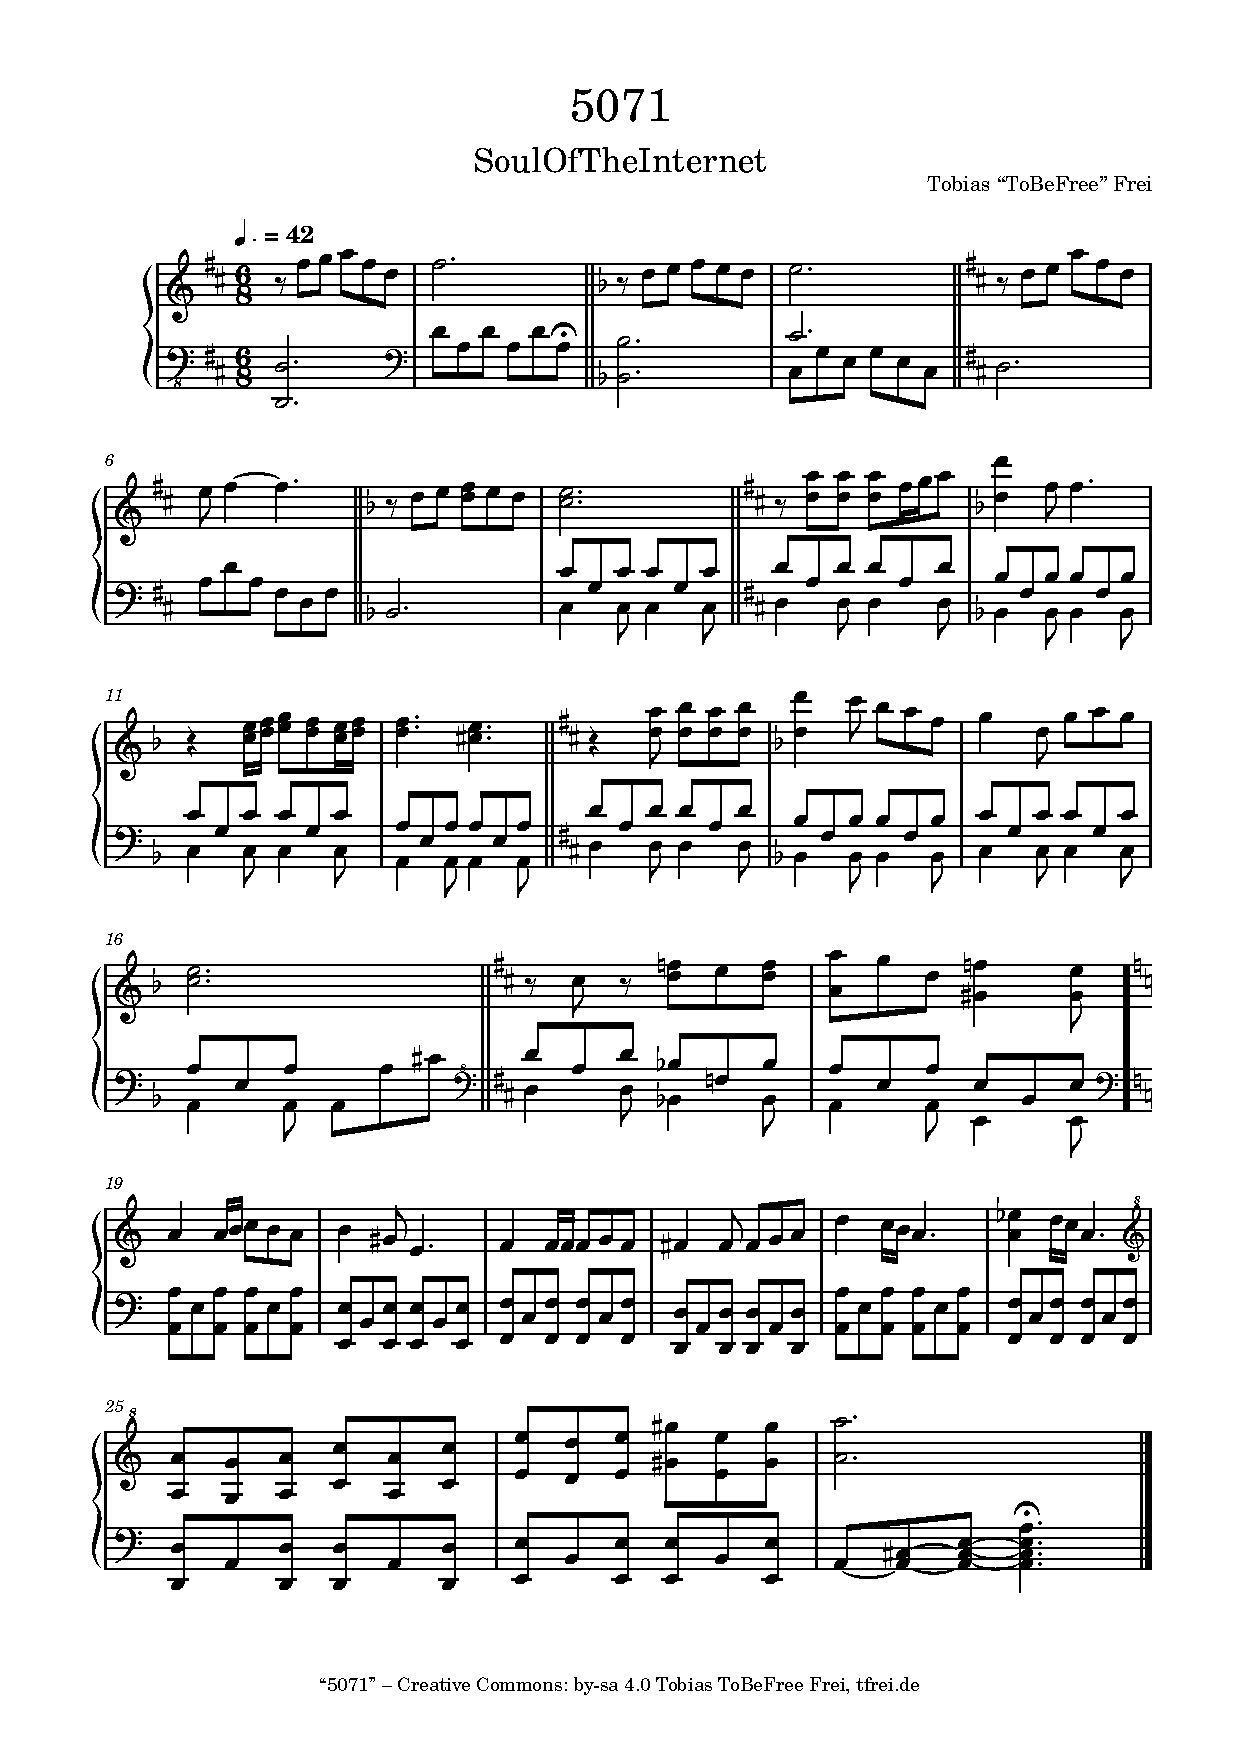
\includegraphics[width=\textwidth, page=1]{z-include-5071theme.pdf}
\end{figure}


\chapter{Musikliste}

\textbf{Für Filmproduzenten, Träumer und Multitasking-Genies.}

\begin{itemize}
    \item Falls Du ernsthaft einen Film zu diesem Buch drehen möchtest.
    \item Falls Du das gesamte Buch bereits ausgelesen hast und die genannten Lieder vielleicht noch nicht kennst. Höre die Lieder und stelle Dir dabei die Szenen vor. Wenn es schon keinen 5071-Film gibt, kannst Du wenigstens einen Film in deinem Kopf laufen lassen.
    \item Falls Du beim Lesen Musik hören möchtest, die zur aktuellen Szene passt.
\end{itemize}

Diese Liste wurde von Tobias Frei zusammengestellt und impliziert keinerlei Unterstützung oder Befürwortung durch die Komponisten der Lieder. Eines Tages wird jedes dieser Lieder in die Gemeinfreiheit übergehen; der genaue Zeitpunkt hängt von verschiedenen Gesetzen ab.

\begin{enumerate}
    \item Titelmelodie:\\ »5071«~– Tobias »ToBeFree« Frei
    \item \textbf{Teil 1: 50.}\\ »Running to the Edge«~– Beyond the Black
    \item Gläserne Gebäudefronten:\\ »What I’ve Done«~– Linkin Park
    \item Raumhafen:\\ »Nobody’s Home«~– Avril Lavigne
    \item Spaziergang vom Raumhafen in die Stadt:\\ »Army of Dolls«~– Delain
    \item Hocksitz:\\ »The Island«~– Ladytron
    \item Erkenntnisgewinn:\\ »Dangerous (featuring Joywave)«~– Big Data
    \item Das Hochhaus:\\ »You’ve Changed«~– Ladytron
    \item Verlassen des Gefängnisplaneten:\\ »Freestate«~– Depeche Mode
    \item Flammender Empfang:\\ »Figurine«~– Ladytron
    \item Sonnenschein am Strand:\\ »Lonely Boy«~– The Black Keys
    \item Hoteldiskussionen:\\ »Tomorrow«~– Ladytron
    \item Verfolgungsjagd zum Raumhafen:\\ »Sweet Tooth«~– Scott Helman
    \item Verfolgungsjagd ins All:\\ »Ready for the Fire«~– Valley of Wolves
    \item Wahrheitsfindung im Helixnebel:\\ »The Hunter«~– Marnie
    \item Das Restaurant am Ende des Universums:\\ »Miss Misery«~– Elliot Smith
    \item SOTIs Wohnung:\\ »The Wight to Remain«~– Danny Baranowsky
    \item Url löscht das Licht:\\ »You Haven’t Earned It«~– Assemblage 23
    \item Free führt SOTI zum Glashaus:\\ »Alive«~– Assemblage 23
    \item Laserlicht-Apokalypse:\\ »Some Mutts (Can’t Be Muzzled)«~– Amyl and the Sniffers
    \item Nasses Erwachen und düstere Gegenüberstellung:\\ »Damaged«~– Assemblage 23
    \item Der Prozess:\\ »Scarlet Sky«~– Miracle of Sound
    \item Vorbesprechung der Zeitreise, Teil 1:\\ »Lilac and Violet«~– Miracle of Sound
    \item Vorbesprechung der Zeitreise, Teil 2:\\ »Ordinary World«~– Duran Duran
    \item Vorbesprechung der Zeitreise, Teil 3:\\ »Fading Light«~– Aviators
    \item Vorbesprechung der Zeitreise, Teil 4:\\ »My Dark Disquiet«~– Poets of the Fall
    \item \textbf{Teil 2: 71.}\\ »Zeit zu gehen«~– Unheilig
    \item Durch Türen und Steine:\\ »Rasputin«~– Boney M
    \item Müsli und Pizza:\\ »Back from the Dead«~– Halestorm
    \item Betrugspläne und ein weißer Umschlag:\\ »Brightside«~– Halestorm
    \item Toronto, 19. Juni 2024:\\ »All I See Is Darkness«~– Icon for Hire
    \item Dönkwön II, 03. September 2021:\\ »Backseat Boogie«~– Airbourne
    \item Antigravitationstornado:\\ »Ghosts«~– Ladytron
    \item ÖrzKäpitöl, 08. Dezember 2015:\\ »WTF do I know?«~– Miley Cyrus
    \item Dunkelheit in der Raumschiffschleuse:\\ »Wenn die Kälte kommt«~– Santiano
    \item Befreiungschaos:\\ »Bullet Proof«~– Diamante
    \item Willkommen zurück in der Freiheit:\\ »Eden«~– Battle Beast
    \item Romantechnische Besprechung:\\ »Extreme Ways«~– Moby
    \item Alle Türen stehen offen:\\ »Davy Jones«~– Santiano
    \item Abflug zur Erde:\\ »Ode an das Meer«~– Santiano
    \item Landung in Kanada:\\ »Weh mir«~– Santiano
    \item Monongahela National Forest, 02. September 2021:\\ »Moonlight Blue«~– Miracle of Sound featuring Sharm
    \item Merkwürdige Kassenbegegnung:\\ »Durch jeden Sturm (Instrumental)«~– Santiano
    \item Blitz in der Dunkelheit:\\ »Bad Luck«~– Aviators
    \item Erzählerwecker am nächsten Morgen:\\ »Only Happy When It Rains«~– Garbage
    \item Zusammenkunft der Götter:\\ »Disco Descent«~– Danny Baranowsky
    \item SOTI verschwindet:\\ »Modern Mythology«~– Aviators
    \item Selbstbegegnung im Gang:\\ »A Pain That I’m Used To«~– Depeche Mode
    \item Rückweg zur Lichtung:\\ »Go and Know«~– Aavikko
    \item Rückkehr des roten Flitzers:\\ »Let Me Be Your Armor«~– Assemblage 23
    \item Kältegefühl:\\ »Winter Is Coming«~– Beyond the Black
    \item SOTI und SOTI:\\ »Paper Highways«~– Ladytron
    \item Rückreise nach Kanada:\\ »Song of the Abyss«~– Aviators
    \item Zwischen den Welten:\\ »Falling Stars«~– Aviators
    \item Schreck im Silber:\\ »Wicked Ways«~– Halestorm
    \item Besprechung in Eitelkeit:\\ »Bad List«~– Ayria
    \item Übergabe des Umschlags:\\ »Document«~– Assemblage 23
    \item Abschied in Einsamkeit:\\ »Legenden«~– dArtagnan
    \item Maia I:\\ »Ordinary World«~– Duran Duran
    \item Zielbesprechung im Dunkeln:\\ »The Noise Inside My Head«~– Assemblage 23
    \item Örz, 05. Oktober 2109:\\ »Blue Jeans«~– Ladytron
    \item Örz, 05. Oktober 2036:\\ »Thunderstruck«~– AC/DC
    \item Anfang und Ende der Welt:\\ »Is There Anybody Out There?«~– Beyond the Black
    \item Versöhnung:\\ »The Quest and the Curse«~– Delain
    \item Finale:\\ »Behind Blue Eyes«~– Limp Bizkit
    \item Outro:\\ »Vielleicht Irgendwann«~– Vincent Weiss
    \item Postskriptum:\\ »Deadzone«~– Ladytron
    \item Rückblick:\\ »Alpenglow«~– Nightwish
\end{enumerate}

Musik, die leider nicht mehr in die Musikliste gepasst hat:

\begin{itemize}
    \item »Horizons«~– Beyond the Black
    \item »Parade«~– Beyond the Black
    \item Untergang des fremden Sternenreichs, Teil 1:\\ »The Tragedy of the Commons«~– Delain
    \item Untergang des fremden Sternenreichs, Teil 2:\\ »Lullaby«~– Delain
    \item »Here come the Vultures«~– Delain
    \item »Shadow«~– Icon for Hire
    \item »Destroy Everything You Touch«~– Ladytron
    \item »The Animals«~– Ladytron
    \item »Lessons in Love«~– Level 42
    \item »Midnight Sky«~– Miley Cyrus
    \item »Night Crawling«~– Miley Cyrus
    \item »Lift me Up«~– Moby
    \item »You Might Think«~– The Cars
    \item »Durch den Sturm«~– Versengold
\end{itemize}


\chapter{Bildquellen}

Alle verwendeten Bilder sind gemeinfrei. Die Verwendung der Bilder in diesem Roman impliziert keinerlei Unterstützung oder Befürwortung durch ihre Schöpfer.

\begin{itemize}
    \item \textbf{Die Seele des Internets.}\\ (Buchcover; Titelbild des zweiten Teils)\\ gemeinfrei
\end{itemize}

Ich bin mir nicht sicher, was du in diesem Kapitel erwartet hast. Hoffentlich gefällt es dir trotzdem.


\chapter{Lizenz des Buchinhalts}

\textbf{5071 © by\\ Tobias Frei, 5071.de}

Dies ist eine offizielle Ausgabe des Romans 5071, herausgegeben von Tobias Frei. Veränderte Versionen und unautorisierte Nachdrucke müssen deutlich als solche erkennbar sein. Auch das Impressum muss angepasst werden, wenn das Dokument verändert wird.

Falls du die Rechte in dieser Lizenz nutzen möchtest, musst du sie vollständig gelesen und verstanden haben. Es genügt nicht, nur eine Zusammenfassung zu lesen. Aus diesem Grund wird in diesem Buch keine Zusammenfassung angeboten.

This novel is licensed under a Creative Commons Attribution-ShareAlike 4.0 International License.

You should have received a copy of the license along with this work. If not, see\\
https://creativecommons.org/licenses/by-sa/4.0/legalcode

You are required to actually read and understand the full text of the license, not a summary.

\begin{center}
    \large{\textbf{Creative Commons Attribution-ShareAlike 4.0 International Public License}}
\end{center}

By exercising the Licensed Rights (defined below), You accept and agree to be bound by the terms and conditions of this Creative Commons Attribution-ShareAlike 4.0 International Public License ("Public License"). To the extent this Public License may be interpreted as a contract, You are granted the Licensed Rights in consideration of Your acceptance of these terms and conditions, and the Licensor grants You such rights in consideration of benefits the Licensor receives from making the Licensed Material available under these terms and conditions.

\begin{center}
    \textbf{Section 1 -- Definitions.}
\end{center}

\begin{itemize}
    \item[a.] \textbf{Adapted Material} means material subject to Copyright and Similar Rights that is derived from or based upon the Licensed Material and in which the Licensed Material is translated, altered, arranged, transformed, or otherwise modified in a manner requiring permission under the Copyright and Similar Rights held by the Licensor. For purposes of this Public License, where the Licensed Material is a musical work, performance, or sound recording, Adapted Material is always produced where the Licensed Material is synched in timed relation with a moving image.
    \item[b.] \textbf{Adapter's License} means the license You apply to Your Copyright and Similar Rights in Your contributions to Adapted Material in accordance with the terms and conditions of this Public License.
    \item[c.] \textbf{BY-SA Compatible License} means a license listed at creativecommons.org/compatiblelicenses, approved by Creative Commons as essentially the equivalent of this Public License.
    \item[d.] \textbf{Copyright and Similar Rights} means copyright and/or similar rights closely related to copyright including, without limitation, performance, broadcast, sound recording, and Sui Generis Database Rights, without regard to how the rights are labeled or categorized. For purposes of this Public License, the rights specified in Section 2(b)(1)-(2) are not Copyright and Similar Rights.
    \item[e.] \textbf{Effective Technological Measures} means those measures that, in the absence of proper authority, may not be circumvented under laws fulfilling obligations under Article 11 of the WIPO Copyright Treaty adopted on December 20, 1996, and/or similar international agreements.
    \item[f.] \textbf{Exceptions and Limitations} means fair use, fair dealing, and/or any other exception or limitation to Copyright and Similar Rights that applies to Your use of the Licensed Material.
    \item[g.] \textbf{License Elements} means the license attributes listed in the name of a Creative Commons Public License. The License Elements of this Public License are Attribution and ShareAlike.
    \item[h.] \textbf{Licensed Material} means the artistic or literary work, database, or other material to which the Licensor applied this Public License.
    \item[i.] \textbf{Licensed Rights} means the rights granted to You subject to the terms and conditions of this Public License, which are limited to all Copyright and Similar Rights that apply to Your use of the Licensed Material and that the Licensor has authority to license.
    \item[j.] \textbf{Licensor} means the individual(s) or entity(ies) granting rights under this Public License.
    \item[k.] \textbf{Share} means to provide material to the public by any means or process that requires permission under the Licensed Rights, such as reproduction, public display, public performance, distribution, dissemination, communication, or importation, and to make material available to the public including in ways that members of the public may access the material from a place and at a time individually chosen by them.
    \item[l.] \textbf{Sui Generis Database Rights} means rights other than copyright resulting from Directive 96/9/EC of the European Parliament and of the Council of 11 March 1996 on the legal protection of databases, as amended and/or succeeded, as well as other essentially equivalent rights anywhere in the world.
    \item[m.] \textbf{You} means the individual or entity exercising the Licensed Rights under this Public License. Your has a corresponding meaning.
\end{itemize}

\begin{center}
    \textbf{Section 2 -- Scope.}
\end{center}

\begin{itemize}
    \item[a.] \textbf{License grant.}
    \begin{itemize}
        \item[1.] Subject to the terms and conditions of this Public License, the Licensor hereby grants You a worldwide, royalty-free, non-sublicensable, non-exclusive, irrevocable license to exercise the Licensed Rights in the Licensed Material to:
        \begin{itemize}
            \item[A.] reproduce and Share the Licensed Material, in whole or in part; and
            \item[B.] produce, reproduce, and Share Adapted Material.
        \end{itemize}
        \item[2.] \underline{Exceptions and Limitations}. For the avoidance of doubt, where Exceptions and Limitations apply to Your use, this Public License does not apply, and You do not need to comply with its terms and conditions.
        \item[3.] \underline{Term}. The term of this Public License is specified in Section 6(a).
        \item[4.] \underline{Media and formats; technical modifications allowed}. The Licensor authorizes You to exercise the Licensed Rights in all media and formats whether now known or hereafter created, and to make technical modifications necessary to do so. The Licensor waives and/or agrees not to assert any right or authority to forbid You from making technical modifications necessary to exercise the Licensed Rights, including technical modifications necessary to circumvent Effective Technological Measures. For purposes of this Public License, simply making modifications authorized by this Section 2(a)(4) never produces Adapted Material.
        \item[5.] \underline{Downstream recipients}.
        \begin{itshape}\begin{itemize}
            \item[A.] \underline{Offer from the Licensor -- Licensed Material}. Every recipient of the Licensed Material automatically receives an offer from the Licensor to exercise the Licensed Rights under the terms and conditions of this Public License.
            \item[B.] \underline{Additional offer from the Licensor -- Adapted Material}. Every recipient of Adapted Material from You automatically receives an offer from the Licensor to exercise the Licensed Rights in the Adapted Material under the conditions of the Adapter's License You apply.
            \item[C.] \underline{No downstream restrictions}. You may not offer or impose any additional or different terms or conditions on, or apply any Effective Technological Measures to, the Licensed Material if doing so restricts exercise of the Licensed Rights by any recipient of the Licensed Material.
        \end{itemize}\end{itshape}
        \item[6.] \underline{No endorsement}. Nothing in this Public License constitutes or may be construed as permission to assert or imply that You are, or that Your use of the Licensed Material is, connected with, or sponsored, endorsed, or granted official status by, the Licensor or others designated to receive attribution as provided in Section 3(a)(1)(A)(i).
    \end{itemize}
    \item[b.] \textbf{Other rights.}
    \begin{itemize}
        \item[1.] Moral rights, such as the right of integrity, are not licensed under this Public License, nor are publicity,
          privacy, and/or other similar personality rights; however, to the extent possible, the Licensor waives and/or agrees not to assert any such rights held by the Licensor to the limited extent necessary to allow You to exercise the Licensed Rights, but not otherwise.
        \item[2.] Patent and trademark rights are not licensed under this Public License.
        \item[3.] To the extent possible, the Licensor waives any right to collect royalties from You for the exercise of the Licensed Rights, whether directly or through a collecting society under any voluntary or waivable statutory or compulsory licensing scheme. In all other cases the Licensor expressly reserves any right to collect such royalties.
    \end{itemize}
\end{itemize}

\begin{center}
    \textbf{Section 3 -- License Conditions.}
\end{center}

Your exercise of the Licensed Rights is expressly made subject to the following conditions.

\begin{itemize}
    \item[a.] \textbf{Attribution.}
    \begin{itemize}
        \item[1.] If You Share the Licensed Material (including in modified form), You must:
        \begin{itemize}
            \item[A.] retain the following if it is supplied by the Licensor with the Licensed Material:
            \begin{itemize}
                \item[i.] identification of the creator(s) of the Licensed Material and any others designated to receive attribution, in any reasonable manner requested by the Licensor (including by pseudonym if designated);
                \item[ii.] a copyright notice;
                \item[iii.] a notice that refers to this Public License;
                \item[iv.] a notice that refers to the disclaimer of warranties;
                \item[v.] a URI or hyperlink to the Licensed Material to the extent reasonably practicable;
            \end{itemize}
            \item[B.] indicate if You modified the Licensed Material and retain an indication of any previous modifications; and
            \item[C.] indicate the Licensed Material is licensed under this Public License, and include the text of, or the URI or hyperlink to, this Public License.
        \end{itemize}
        \item[2.] You may satisfy the conditions in Section 3(a)(1) in any reasonable manner based on the medium, means, and context in which You Share the Licensed Material. For example, it may be reasonable to satisfy the conditions by providing a URI or hyperlink to a resource that includes the required information.
        \item[3.] If requested by the Licensor, You must remove any of the information required by Section 3(a)(1)(A) to the extent reasonably practicable.
    \end{itemize}
    \item[b.] \textbf{ShareAlike.}

     In addition to the conditions in Section 3(a), if You Share Adapted Material You produce, the following conditions also apply.

    \begin{itemize}
        \item[1.] The Adapter's License You apply must be a Creative Commons license with the same License Elements, this version or later, or a BY-SA Compatible License.
        \item[2.] You must include the text of, or the URI or hyperlink to, the Adapter's License You apply. You may satisfy this condition in any reasonable manner based on the medium, means, and context in which You Share Adapted Material.
        \item[3.] You may not offer or impose any additional or different terms or conditions on, or apply any Effective Technological Measures to, Adapted Material that restrict exercise of the rights granted under the Adapter's License You apply.
    \end{itemize}
\end{itemize}

\begin{center}
    \textbf{Section 4 -- Sui Generis Database Rights.}
\end{center}

Where the Licensed Rights include Sui Generis Database Rights that apply to Your use of the Licensed Material:

\begin{itemize}
    \item[a.] for the avoidance of doubt, Section 2(a)(1) grants You the right to extract, reuse, reproduce, and Share all or a substantial portion of the contents of the database;
    \item[b.] if You include all or a substantial portion of the database contents in a database in which You have Sui Generis Database Rights, then the database in which You have Sui Generis Database Rights (but not its individual contents) is Adapted Material, including for purposes of Section 3(b); and
    \item[c.] You must comply with the conditions in Section 3(a) if You Share all or a substantial portion of the contents of the database.
\end{itemize}

For the avoidance of doubt, this Section 4 supplements and does not replace Your obligations under this Public License where the Licensed Rights include other Copyright and Similar Rights.

\begin{center}
    \textbf{Section 5 -- Disclaimer of Warranties and Limitation of Liability.}
\end{center}

\begin{itemize}
    \item[\textbf{a.}] \textbf{Unless otherwise separately undertaken by the Licensor, to the extent possible, the Licensor offers the Licensed Material as-is and as-available, and makes no representations or warranties of any kind concerning the Licensed Material, whether express, implied, statutory, or other. This includes, without limitation, warranties of title, merchantability, fitness for a particular purpose, non-infringement, absence of latent or other defects, accuracy, or the presence or absence of errors, whether or not known or discoverable. Where disclaimers of warranties are not allowed in full or in part, this disclaimer may not apply to You.}
    \item[\textbf{b.}] \textbf{To the extent possible, in no event will the Licensor be liable to You on any legal theory (including, without limitation, negligence) or otherwise for any direct, special, indirect, incidental, consequential, punitive, exemplary, or other losses, costs, expenses, or damages arising out of this Public License or use of the Licensed Material, even if the Licensor has been advised of the possibility of such losses, costs, expenses, or damages. Where a limitation of liability is not allowed in full or in part, this limitation may not apply to You.}
    \item[c.] The disclaimer of warranties and limitation of liability provided above shall be interpreted in a manner that, to the extent possible, most closely approximates an absolute disclaimer and waiver of all liability.
\end{itemize}

\begin{center}
    \textbf{Section 6 -- Term and Termination.}
\end{center}

\begin{itemize}
    \item[a.] This Public License applies for the term of the Copyright and Similar Rights licensed here. However, if You fail to comply with this Public License, then Your rights under this Public License terminate automatically.
    \item[b.] Where Your right to use the Licensed Material has terminated under Section 6(a), it reinstates:
    \begin{itemize}
        \item[1.] automatically as of the date the violation is cured, provided it is cured within 30 days of Your discovery of the violation; or
        \item[2.] upon express reinstatement by the Licensor.
    \end{itemize}

     For the avoidance of doubt, this Section 6(b) does not affect any right the Licensor may have to seek remedies for Your violations of this Public License.

    \item[c.] For the avoidance of doubt, the Licensor may also offer the Licensed Material under separate terms or conditions or stop distributing the Licensed Material at any time; however, doing so will not terminate this Public License.
    \item[d.] Sections 1, 5, 6, 7, and 8 survive termination of this Public License.
\end{itemize}

\begin{center}
    \textbf{Section 7 -- Other Terms and Conditions.}
\end{center}

\begin{itemize}
    \item[a.] The Licensor shall not be bound by any additional or different terms or conditions communicated by You unless expressly agreed.
    \item[b.] Any arrangements, understandings, or agreements regarding the Licensed Material not stated herein are separate from and independent of the terms and conditions of this Public License.
\end{itemize}

\begin{center}
    \textbf{Section 8 -- Interpretation.}
\end{center}

\begin{itemize}
    \item[a.] For the avoidance of doubt, this Public License does not, and shall not be interpreted to, reduce, limit, restrict, or impose conditions on any use of the Licensed Material that could lawfully be made without permission under this Public License.
    \item[b.] To the extent possible, if any provision of this Public License is deemed unenforceable, it shall be automatically reformed to the minimum extent necessary to make it enforceable. If the provision cannot be reformed, it shall be severed from this Public License without affecting the enforceability of the remaining terms and conditions.
    \item[c.] No term or condition of this Public License will be waived and no failure to comply consented to unless expressly agreed to by the Licensor.
    \item[d.] Nothing in this Public License constitutes or may be interpreted as a limitation upon, or waiver of, any privileges and immunities that apply to the Licensor or You, including from the legal processes of any jurisdiction or authority.
\end{itemize}

\end{document}
